\documentclass[]{book}
\usepackage{lmodern}
\usepackage{amssymb,amsmath}
\usepackage{ifxetex,ifluatex}
\usepackage{fixltx2e} % provides \textsubscript
\ifnum 0\ifxetex 1\fi\ifluatex 1\fi=0 % if pdftex
  \usepackage[T1]{fontenc}
  \usepackage[utf8]{inputenc}
\else % if luatex or xelatex
  \ifxetex
    \usepackage{mathspec}
  \else
    \usepackage{fontspec}
  \fi
  \defaultfontfeatures{Ligatures=TeX,Scale=MatchLowercase}
\fi
% use upquote if available, for straight quotes in verbatim environments
\IfFileExists{upquote.sty}{\usepackage{upquote}}{}
% use microtype if available
\IfFileExists{microtype.sty}{%
\usepackage{microtype}
\UseMicrotypeSet[protrusion]{basicmath} % disable protrusion for tt fonts
}{}
\usepackage[margin=1in]{geometry}
\usepackage{hyperref}
\hypersetup{unicode=true,
            pdftitle={Modern R in a Corporate Environment},
            pdfauthor={Brian Davis},
            pdfborder={0 0 0},
            breaklinks=true}
\urlstyle{same}  % don't use monospace font for urls
\usepackage{natbib}
\bibliographystyle{apalike}
\usepackage{color}
\usepackage{fancyvrb}
\newcommand{\VerbBar}{|}
\newcommand{\VERB}{\Verb[commandchars=\\\{\}]}
\DefineVerbatimEnvironment{Highlighting}{Verbatim}{commandchars=\\\{\}}
% Add ',fontsize=\small' for more characters per line
\usepackage{framed}
\definecolor{shadecolor}{RGB}{248,248,248}
\newenvironment{Shaded}{\begin{snugshade}}{\end{snugshade}}
\newcommand{\KeywordTok}[1]{\textcolor[rgb]{0.13,0.29,0.53}{\textbf{#1}}}
\newcommand{\DataTypeTok}[1]{\textcolor[rgb]{0.13,0.29,0.53}{#1}}
\newcommand{\DecValTok}[1]{\textcolor[rgb]{0.00,0.00,0.81}{#1}}
\newcommand{\BaseNTok}[1]{\textcolor[rgb]{0.00,0.00,0.81}{#1}}
\newcommand{\FloatTok}[1]{\textcolor[rgb]{0.00,0.00,0.81}{#1}}
\newcommand{\ConstantTok}[1]{\textcolor[rgb]{0.00,0.00,0.00}{#1}}
\newcommand{\CharTok}[1]{\textcolor[rgb]{0.31,0.60,0.02}{#1}}
\newcommand{\SpecialCharTok}[1]{\textcolor[rgb]{0.00,0.00,0.00}{#1}}
\newcommand{\StringTok}[1]{\textcolor[rgb]{0.31,0.60,0.02}{#1}}
\newcommand{\VerbatimStringTok}[1]{\textcolor[rgb]{0.31,0.60,0.02}{#1}}
\newcommand{\SpecialStringTok}[1]{\textcolor[rgb]{0.31,0.60,0.02}{#1}}
\newcommand{\ImportTok}[1]{#1}
\newcommand{\CommentTok}[1]{\textcolor[rgb]{0.56,0.35,0.01}{\textit{#1}}}
\newcommand{\DocumentationTok}[1]{\textcolor[rgb]{0.56,0.35,0.01}{\textbf{\textit{#1}}}}
\newcommand{\AnnotationTok}[1]{\textcolor[rgb]{0.56,0.35,0.01}{\textbf{\textit{#1}}}}
\newcommand{\CommentVarTok}[1]{\textcolor[rgb]{0.56,0.35,0.01}{\textbf{\textit{#1}}}}
\newcommand{\OtherTok}[1]{\textcolor[rgb]{0.56,0.35,0.01}{#1}}
\newcommand{\FunctionTok}[1]{\textcolor[rgb]{0.00,0.00,0.00}{#1}}
\newcommand{\VariableTok}[1]{\textcolor[rgb]{0.00,0.00,0.00}{#1}}
\newcommand{\ControlFlowTok}[1]{\textcolor[rgb]{0.13,0.29,0.53}{\textbf{#1}}}
\newcommand{\OperatorTok}[1]{\textcolor[rgb]{0.81,0.36,0.00}{\textbf{#1}}}
\newcommand{\BuiltInTok}[1]{#1}
\newcommand{\ExtensionTok}[1]{#1}
\newcommand{\PreprocessorTok}[1]{\textcolor[rgb]{0.56,0.35,0.01}{\textit{#1}}}
\newcommand{\AttributeTok}[1]{\textcolor[rgb]{0.77,0.63,0.00}{#1}}
\newcommand{\RegionMarkerTok}[1]{#1}
\newcommand{\InformationTok}[1]{\textcolor[rgb]{0.56,0.35,0.01}{\textbf{\textit{#1}}}}
\newcommand{\WarningTok}[1]{\textcolor[rgb]{0.56,0.35,0.01}{\textbf{\textit{#1}}}}
\newcommand{\AlertTok}[1]{\textcolor[rgb]{0.94,0.16,0.16}{#1}}
\newcommand{\ErrorTok}[1]{\textcolor[rgb]{0.64,0.00,0.00}{\textbf{#1}}}
\newcommand{\NormalTok}[1]{#1}
\usepackage{longtable,booktabs}
\usepackage{graphicx,grffile}
\makeatletter
\def\maxwidth{\ifdim\Gin@nat@width>\linewidth\linewidth\else\Gin@nat@width\fi}
\def\maxheight{\ifdim\Gin@nat@height>\textheight\textheight\else\Gin@nat@height\fi}
\makeatother
% Scale images if necessary, so that they will not overflow the page
% margins by default, and it is still possible to overwrite the defaults
% using explicit options in \includegraphics[width, height, ...]{}
\setkeys{Gin}{width=\maxwidth,height=\maxheight,keepaspectratio}
\IfFileExists{parskip.sty}{%
\usepackage{parskip}
}{% else
\setlength{\parindent}{0pt}
\setlength{\parskip}{6pt plus 2pt minus 1pt}
}
\setlength{\emergencystretch}{3em}  % prevent overfull lines
\providecommand{\tightlist}{%
  \setlength{\itemsep}{0pt}\setlength{\parskip}{0pt}}
\setcounter{secnumdepth}{5}
% Redefines (sub)paragraphs to behave more like sections
\ifx\paragraph\undefined\else
\let\oldparagraph\paragraph
\renewcommand{\paragraph}[1]{\oldparagraph{#1}\mbox{}}
\fi
\ifx\subparagraph\undefined\else
\let\oldsubparagraph\subparagraph
\renewcommand{\subparagraph}[1]{\oldsubparagraph{#1}\mbox{}}
\fi

%%% Use protect on footnotes to avoid problems with footnotes in titles
\let\rmarkdownfootnote\footnote%
\def\footnote{\protect\rmarkdownfootnote}

%%% Change title format to be more compact
\usepackage{titling}

% Create subtitle command for use in maketitle
\newcommand{\subtitle}[1]{
  \posttitle{
    \begin{center}\large#1\end{center}
    }
}

\setlength{\droptitle}{-2em}

  \title{Modern R in a Corporate Environment}
    \pretitle{\vspace{\droptitle}\centering\huge}
  \posttitle{\par}
  \subtitle{R course developed for the office}
  \author{Brian Davis}
    \preauthor{\centering\large\emph}
  \postauthor{\par}
      \predate{\centering\large\emph}
  \postdate{\par}
    \date{2019-01-11}

\usepackage{booktabs}
\usepackage{longtable}
\usepackage{framed,color}
\definecolor{shadecolor}{RGB}{248,248,248}

\ifxetex
  \usepackage{letltxmacro}
  \setlength{\XeTeXLinkMargin}{1pt}
  \LetLtxMacro\SavedIncludeGraphics\includegraphics
  \def\includegraphics#1#{% #1 catches optional stuff (star/opt. arg.)
    \IncludeGraphicsAux{#1}%
  }%
  \newcommand*{\IncludeGraphicsAux}[2]{%
    \XeTeXLinkBox{%
      \SavedIncludeGraphics#1{#2}%
    }%
  }%
\fi

\newenvironment{rmdblock}[1]
  {\begin{shaded*}
  \begin{itemize}
  \renewcommand{\labelitemi}{
    \raisebox{-.7\height}[0pt][0pt]{
      {\setkeys{Gin}{width=3em,keepaspectratio}\includegraphics{images/#1}}
    }
  }
  \item
  }
  {
  \end{itemize}
  \end{shaded*}
  }
\newenvironment{rmdnote}
  {\begin{rmdblock}{note}}
  {\end{rmdblock}}
\newenvironment{rmdtip}
  {\begin{rmdblock}{tip}}
  {\end{rmdblock}}
\newenvironment{rmdwarning}
  {\begin{rmdblock}{warning}}
  {\end{rmdblock}}
\newenvironment{rmdcaution}
  {\begin{rmdblock}{caution}}
  {\end{rmdblock}}
  \newenvironment{rmdimportant}
  {\begin{rmdblock}{important}}
  {\end{rmdblock}}
  
\usepackage{amsthm}
\makeatletter
\def\thm@space@setup{%
  \thm@preskip=8pt plus 2pt minus 4pt
  \thm@postskip=\thm@preskip
}
\makeatother
\usepackage{booktabs}
\usepackage{longtable}
\usepackage{array}
\usepackage{multirow}
\usepackage[table]{xcolor}
\usepackage{wrapfig}
\usepackage{float}
\usepackage{colortbl}
\usepackage{pdflscape}
\usepackage{tabu}
\usepackage{threeparttable}
\usepackage{threeparttablex}
\usepackage[normalem]{ulem}
\usepackage{makecell}

\let\BeginKnitrBlock\begin \let\EndKnitrBlock\end
\begin{document}
\maketitle

{
\setcounter{tocdepth}{1}
\tableofcontents
}
\chapter*{Welcome}\label{welcome}
\addcontentsline{toc}{chapter}{Welcome}

\begin{quote}
Something that will make life easier in the long-run can be the most
difficult thing to do today. For coders, prioritising the long term may
involve an overhaul of current practice and the learning of a new skill.
\end{quote}

This is the course notes for our class. This course will teach you how
to do data science with R. You'll learn the basics of R and then we'll
go through \href{http://r4ds.had.co.nz/index.html}{R for Data Science}
by Garrett Grolemund \& Hadley Wickham. You'll learn how to get your
data into R, get it into the most useful structure, transform it,
visualize it and communicate out your results. We'll mix in various
topics from our current workload as well as some unique challenges of
working in a corporate environment.

Most of these are the skills that allow data science to happen, and here
you will find the best practices for doing each of these things with R.
You'll learn how to use the grammar of graphics, literate programming,
and reproducible research to save time and reduce errors.

We will build the tools to make our work easier and more streamlined
together.

\part{Preamble}\label{part-preamble}

\chapter{Introduction}\label{preamble-intro}

\section{Course Philosophy}\label{course-philosophy}

\begin{quote}
``The best programs are written so that computing machines can perform
them quickly and so that human beings can understand them clearly. A
programmer is ideally an essayist who works with traditional aesthetic
and literary forms as well as mathematical concepts, to communicate the
way that an algorithm works and to convince a reader that the results
will be correct.''

--- Donald Knuth
\end{quote}

\subsection{Reproducible Research
Approach}\label{reproducible-research-approach}

\href{https://www.coursera.org/learn/reproducible-research/lecture/FvOGB/what-is-reproducible-research-about}{What
is Reproducible Research About?}

Reproducible research is the idea that data analyses, and more
generally, scientific claims, are published with their data and software
code so that others may verify the findings and build upon them. There
are two basic reasons to be concerned about making your research
reproducible. The first is \emph{to show evidence of the correctness of
your results}. The second reason to aspire to reproducibility is
\emph{to enable others to make use of our methods and results}.

Modern challenges of reproducibility in research, particularly
computational reproducibility, have produced a lot of discussion in
papers, blogs and videos, some of which are listed
\href{http://ropensci.github.io/reproducibility-guide/sections/references/}{here}
and \href{https://reproducibleresearch.net/}{here}.

\begin{quote}
Conclusions in experimental psychology often are the result of null
hypothesis significance testing. Unfortunately, there is evidence ((from
eight major psychology journals published between 1985 and 2013) that
roughly half of all published empirical psychology articles contain at
least one inconsistent p-value, and around one in eight articles contain
a grossly inconsistent p-value that makes a non-significant result seem
significant, or vice versa.
\href{https://mbnuijten.com/statcheck/}{statscheck} and
\href{http://blog.revolutionanalytics.com/2016/10/statcheck.html}{here}
\end{quote}

\begin{quote}
``A key component of scientific communication is sufficient information
for other researchers in the field to reproduce published findings. For
computational and data-enabled research, this has often been interpreted
to mean making available the raw data from which results were generated,
the computer code that generated the findings, and any additional
information needed such as workflows and input parameters. Many journals
are revising author guidelines to include data and code availability. We
chose a random sample of 204 scientific papers published in the journal
\textbf{Science} after the implementation of their policy in February
2011. We found that were able to reproduce the findings for 26\%.''
\href{http://www.pnas.org/content/115/11/2584}{Proceedings of the
National Academy of Sciences of the United States of America}
\end{quote}

\begin{quote}
``Starting September 1 2016, JASA ACS will require code and data as a
minimum standard for reproducibility of statistical scientific
research.''
\href{https://magazine.amstat.org/blog/2016/07/01/jasa-reproducible16/}{JASA}
\end{quote}

\subsection{FDA Validation}\label{fda-validation}

\begin{quote}
``Establishing documented evidence which provides a high degree of
assurance that a specific process will consistently produce a product
meeting its predetermined specifications and quality attributes.''
-Validation as defined by the FDA in \textbf{Validation of Systems for
21 CFR Part 11 Compliance}
\end{quote}

\subsection{The SAS Myth}\label{the-sas-myth}

Contrary to what we hear the FDA does not require SAS to be used
\emph{EVER}. There are instances that you have to deliver data in XPORT
format though which is open and implemented in many programming
languages.

\begin{quote}
``FDA does not require use of any specific software for statistical
analyses, and statistical software is not explicitly discussed in Title
21 of the Code of Federal Regulations {[}e.g., in 21CFR part 11{]}.
However, the software package(s) used for statistical analyses should be
fully documented in the submission, including version and build
identification. As noted in the FDA guidance, E9 Statistical Principles
for Clinical Trials''
\href{https://www.fda.gov/downloads/forindustry/datastandards/studydatastandards/ucm587506.pdf}{FDA
Statistical Software Clarifying Statement}
\end{quote}

Good \href{http://blog.revolutionanalytics.com/2017/06/r-fda.html}{write
up} with links to several FDA talks on the
\href{https://thomaswdinsmore.com/2014/12/01/sas-versus-r-part-1/}{subject}.

\section{Prerequisites}\label{prerequisites}

\begin{itemize}
\tightlist
\item
  We will assume you have minimal experience and knowledge of R
\item
  IT should have installed:

  \begin{itemize}
  \tightlist
  \item
    \href{https://cran.r-project.org/}{R} version 3.5.1
  \item
    \href{https://www.rstudio.com/products/rstudio/download/\#download}{RStudio}
    version 1.1
  \item
    \href{https://miktex.org/}{MiTeX}
  \item
    \href{https://cran.r-project.org/bin/windows/Rtools/}{RTools}
    version 3.4
  \end{itemize}
\item
  We will install other dependencies throughout the course.
\end{itemize}

\section{Content}\label{content}

It is impossible to become an expert in R in only one course even a
multi-week one. Our aim is at gaining a wide understanding on many
aspects of R as used in a corporate / production environment. It will
roughly be based on \href{http://r4ds.had.co.nz}{R for Data Science}.
While this is an \emph{excellent} resource it does not cover much of
what we will need on a routine basis. Some external resources will be
referred to in this book for you to be able to deepen what you would
have learned in this course.

We will focus most of our attention to the \emph{tidyverse} family of
packages for data analysis. The \emph{tidyverse} is an opinionated
\href{https://www.tidyverse.org/packages/}{collection of R packages}
designed for data science. All packages share an underlying design
philosophy, grammar, and data structures.

This is your course so if you feel we need to hit an area deeper, or add
content based on a current need, let me know an we will work to adjust
it.

The \textbf{rough} topic list of the course:

\begin{enumerate}
\def\labelenumi{\arabic{enumi}.}
\tightlist
\item
  Good programming practices
\item
  Basics of R Programming
\item
  Importing / Exporting Data
\item
  Tidying Data
\item
  Visualizing Data
\item
  Functions
\item
  Strings
\item
  Dates and Time
\item
  Communicating Results
\item
  Iteration
\end{enumerate}

\section{Structure}\label{structure}

My current thoughts are to meet an hour a week and discuss a topic. We
will not be going strictly through the R4DS, but will use it as our
foundation into the topic at hand. Then give some exercises due for the
next week which we go over the solutions. We will incorporate these
exercises into an R package(s?) so we will have a collection of useful
reusable code for the future.

Open to other ideas as we go along.

I'm going to try to keep the assignments related to our current work so
we can work on the class during work hours. Bring what you are working
on and we will see how we can fit it into the class.

\chapter{Good practices}\label{good-practices}

\begin{quote}
``When you write a program, think of it primarily as a work of
literature. You're trying to write something that human beings are going
to read. Don't think of it primarily as something a computer is going to
follow. The more effective you are at making your program readable, the
more effective it's going to be: You'll understand it today, you'll
understand it next week, and your successors who are going to maintain
and modify it will understand it.''

-- Donald Knuth
\end{quote}

\section{Coding style}\label{coding-style}

Good coding style is like correct punctuation: you can manage without
it, butitsuremakesthingseasiertoread. When I answer questions; first, I
see if think I can answer the question, secondly, I check the coding
style of the question and if the code is too difficult to read, I just
move on. Please make your code readable by following e.g.
\href{http://style.tidyverse.org/}{this coding style} (most examples
below come from this guide).

\begin{quote}
``To become ssignificantly more reliable, code must become more
transparent. In particular, nested conditions and loops must be viewed
with great suspicion. Complicated control flows confuse programmers.
\textbf{Messy code often hides bugs}.''

--- Bjarne Stroustrup
\end{quote}

\subsection{Comments}\label{comments}

In code, use comments to explain the ``why'' not the ``what'' or
``how''. Each line of a comment should begin with the comment symbol and
a single space: \texttt{\#}.

\BeginKnitrBlock{rmdtip}
Use commented lines of - to break up your file into easily readable
chunks and to create a code outline in RStudio
\EndKnitrBlock{rmdtip}

\subsection{Naming}\label{naming}

\begin{quote}
There are only two hard things in Computer Science: cache invalidation
and naming things.

-- Phil Karlton
\end{quote}

Names are not limited to 8 characters as in some other languages,
however they are case sensitive. Be smart with your naming; be
descriptive yet concise. Think about how your names will show up in auto
complete.

Throughout the course we will point out some standard naming conventions
that are used in R (and other languages). (Ex. \texttt{i} and \texttt{j}
as row and column indices)

\begin{Shaded}
\begin{Highlighting}[]
\CommentTok{# Good}
\NormalTok{average_height <-}\StringTok{ }\KeywordTok{mean}\NormalTok{((feet }\OperatorTok{/}\StringTok{ }\DecValTok{12}\NormalTok{) }\OperatorTok{+}\StringTok{ }\NormalTok{inches)}
\KeywordTok{plot}\NormalTok{(mtcars}\OperatorTok{$}\NormalTok{disp, mtcars}\OperatorTok{$}\NormalTok{mpg)}

\CommentTok{# Bad}
\NormalTok{ah<-}\KeywordTok{mean}\NormalTok{(x}\OperatorTok{/}\DecValTok{12}\OperatorTok{+}\NormalTok{y)}
\KeywordTok{plot}\NormalTok{(mtcars[, }\DecValTok{3}\NormalTok{], mtcars[, }\DecValTok{1}\NormalTok{])}
\end{Highlighting}
\end{Shaded}

\subsection{Spacing}\label{spacing}

Put a space before and after \texttt{=} when naming arguments in
function calls. Most infix operators (\texttt{==}, \texttt{+},
\texttt{-}, \texttt{\textless{}-}, etc.) are also surrounded by spaces,
except those with relatively high precedence: \texttt{\^{}}, \texttt{:},
\texttt{::}, and \texttt{:::}. Always put a space after a comma, and
never before (just like in regular English).

\begin{Shaded}
\begin{Highlighting}[]
\CommentTok{# Good}
\NormalTok{average <-}\StringTok{ }\KeywordTok{mean}\NormalTok{((feet }\OperatorTok{/}\StringTok{ }\DecValTok{12}\NormalTok{) }\OperatorTok{+}\StringTok{ }\NormalTok{inches, }\DataTypeTok{na.rm =} \OtherTok{TRUE}\NormalTok{)}
\KeywordTok{sqrt}\NormalTok{(x}\OperatorTok{^}\DecValTok{2} \OperatorTok{+}\StringTok{ }\NormalTok{y}\OperatorTok{^}\DecValTok{2}\NormalTok{)}
\NormalTok{x <-}\StringTok{ }\DecValTok{1}\OperatorTok{:}\DecValTok{10}
\NormalTok{base}\OperatorTok{::}\NormalTok{sum}

\CommentTok{# Bad}
\NormalTok{average<-}\KeywordTok{mean}\NormalTok{(feet}\OperatorTok{/}\DecValTok{12}\OperatorTok{+}\NormalTok{inches,}\DataTypeTok{na.rm=}\OtherTok{TRUE}\NormalTok{)}
\KeywordTok{sqrt}\NormalTok{(x }\OperatorTok{^}\StringTok{ }\DecValTok{2} \OperatorTok{+}\StringTok{ }\NormalTok{y }\OperatorTok{^}\StringTok{ }\DecValTok{2}\NormalTok{)}
\NormalTok{x <-}\StringTok{ }\DecValTok{1} \OperatorTok{:}\StringTok{ }\DecValTok{10}
\NormalTok{base }\OperatorTok{::}\StringTok{ }\NormalTok{sum}
\end{Highlighting}
\end{Shaded}

\subsection{Indenting}\label{indenting}

Curly braces, \texttt{\{\}}, define the the most important hierarchy of
R code. To make this hierarchy easy to see, always indent the code
inside \texttt{\{\}} by two spaces.

\begin{Shaded}
\begin{Highlighting}[]
\CommentTok{# Good}
\ControlFlowTok{if}\NormalTok{ (y }\OperatorTok{<}\StringTok{ }\DecValTok{0} \OperatorTok{&&}\StringTok{ }\NormalTok{debug) \{}
  \KeywordTok{message}\NormalTok{(}\StringTok{"y is negative"}\NormalTok{)}
\NormalTok{\}}

\ControlFlowTok{if}\NormalTok{ (y }\OperatorTok{==}\StringTok{ }\DecValTok{0}\NormalTok{) \{}
  \ControlFlowTok{if}\NormalTok{ (x }\OperatorTok{>}\StringTok{ }\DecValTok{0}\NormalTok{) \{}
    \KeywordTok{log}\NormalTok{(x)}
\NormalTok{  \} }\ControlFlowTok{else}\NormalTok{ \{}
    \KeywordTok{message}\NormalTok{(}\StringTok{"x is negative or zero"}\NormalTok{)}
\NormalTok{  \}}
\NormalTok{\} }\ControlFlowTok{else}\NormalTok{ \{}
\NormalTok{  y }\OperatorTok{^}\StringTok{ }\NormalTok{x}
\NormalTok{\}}

\CommentTok{# Bad}
\ControlFlowTok{if}\NormalTok{ (y }\OperatorTok{<}\StringTok{ }\DecValTok{0} \OperatorTok{&&}\StringTok{ }\NormalTok{debug)}
\KeywordTok{message}\NormalTok{(}\StringTok{"Y is negative"}\NormalTok{)}

\ControlFlowTok{if}\NormalTok{ (y }\OperatorTok{==}\StringTok{ }\DecValTok{0}\NormalTok{)}
\NormalTok{\{}
    \ControlFlowTok{if}\NormalTok{ (x }\OperatorTok{>}\StringTok{ }\DecValTok{0}\NormalTok{) \{}
      \KeywordTok{log}\NormalTok{(x)}
\NormalTok{    \} }\ControlFlowTok{else}\NormalTok{ \{}
  \KeywordTok{message}\NormalTok{(}\StringTok{"x is negative or zero"}\NormalTok{)}
\NormalTok{    \}}
\NormalTok{\} }\ControlFlowTok{else}\NormalTok{ \{ y }\OperatorTok{^}\StringTok{ }\NormalTok{x \}}
\end{Highlighting}
\end{Shaded}

\subsection{Long lines}\label{long-lines}

Strive to limit your code to 80 characters per line. This fits
comfortably on a printed page with a reasonably sized font. If you find
yourself running out of room, this is a good indication that you should
encapsulate some of the work into a separate function.

If a function call is too long to fit on a single line, use one line
each for the function name, each argument, and the closing \texttt{)}.
This makes the code easier to read and to change later.

\begin{Shaded}
\begin{Highlighting}[]
\CommentTok{# Good}
\KeywordTok{do_something_very_complicated}\NormalTok{(}
  \DataTypeTok{something =} \StringTok{"that"}\NormalTok{,}
  \DataTypeTok{requires  =}\NormalTok{ many,}
  \DataTypeTok{arguments =} \StringTok{"some of which may be long"}
\NormalTok{)}

\CommentTok{# Bad}
\KeywordTok{do_something_very_complicated}\NormalTok{(}\StringTok{"that"}\NormalTok{, requires, many, arguments,}
                              \StringTok{"some of which may be long"}
\end{Highlighting}
\end{Shaded}

\subsection{Other}\label{other}

\begin{itemize}
\tightlist
\item
  Use \texttt{\textless{}-}, not \texttt{=}, for assignment. Keep
  \texttt{=} for parameters.
\end{itemize}

\begin{Shaded}
\begin{Highlighting}[]
\CommentTok{# Good}
\NormalTok{x <-}\StringTok{ }\DecValTok{5}
\KeywordTok{system.time}\NormalTok{(}
\NormalTok{  x <-}\StringTok{ }\KeywordTok{rnorm}\NormalTok{(}\FloatTok{1e6}\NormalTok{)}
\NormalTok{)}

\CommentTok{# Bad}
\NormalTok{x =}\StringTok{ }\DecValTok{5}
\KeywordTok{system.time}\NormalTok{(}
  \DataTypeTok{x =} \KeywordTok{rnorm}\NormalTok{(}\FloatTok{1e6}\NormalTok{)}
\NormalTok{)}
\end{Highlighting}
\end{Shaded}

\begin{itemize}
\item
  Don't put \texttt{;} at the end of a line, and don't use \texttt{;} to
  put multiple commands on one line.
\item
  Only use \texttt{return()} for early returns. Otherwise rely on R to
  return the result of the last evaluated expression.
\end{itemize}

\begin{Shaded}
\begin{Highlighting}[]
\CommentTok{# Good}
\NormalTok{add_two <-}\StringTok{ }\ControlFlowTok{function}\NormalTok{(x, y) \{}
\NormalTok{  x }\OperatorTok{+}\StringTok{ }\NormalTok{y}
\NormalTok{\}}

\CommentTok{# Bad}
\NormalTok{add_two <-}\StringTok{ }\ControlFlowTok{function}\NormalTok{(x, y) \{}
  \KeywordTok{return}\NormalTok{(x }\OperatorTok{+}\StringTok{ }\NormalTok{y)}
\NormalTok{\}}
\end{Highlighting}
\end{Shaded}

\begin{itemize}
\tightlist
\item
  Use \texttt{"}, not \texttt{\textquotesingle{}}, for quoting text. The
  only exception is when the text already contains double quotes and no
  single quotes.
\end{itemize}

\begin{Shaded}
\begin{Highlighting}[]
\CommentTok{# Good}
\StringTok{"Text"}
\StringTok{'Text with "quotes"'}
\StringTok{'<a href="http://style.tidyverse.org">A link</a>'}

\CommentTok{# Bad}
\StringTok{'Text'}
\StringTok{'Text with "double" and }\CharTok{\textbackslash{}'}\StringTok{single}\CharTok{\textbackslash{}'}\StringTok{ quotes'}
\end{Highlighting}
\end{Shaded}

\section{Coding practices}\label{coding-practices}

\subsection{Variables}\label{variables}

Create variables for values that are likely to change.

\subsection[\emph{Rule of Three}]{\texorpdfstring{\emph{Rule of
Three}\footnote{This is sometimes called the DRY principle, or Don't
  Repeat Yourself.}}{Rule of Three}}\label{rule-of-threedry}

Try not to copy code, or copy then modify the code, more than twice.

\begin{itemize}
\tightlist
\item
  If a change requires you to search/replace 3 or more times \emph{make
  a variable}.
\item
  If you copy a code chunk 3 or more times \emph{make a function}
\item
  If you copy a function 3 or more times \emph{make your function more
  generic}
\item
  If you copy a function into a project 3 or more times \emph{make a
  package}
\item
  If 3 or more people will use the function \emph{make a package}
\end{itemize}

The \emph{Rule of Three} applies to look-up tables and such also. The
key thing to think about is; if something changes how many touch points
will there be? If it is 3 or more places it is time to abstract this
code a bit.

\subsection{Path names}\label{path-names}

It is better to use relative path names instead of hard coded ones. If
you must read from (or write to) paths that are not in your project
directory structure create a file name variable at the highest level you
can (\emph{always end with the \texttt{/}}) and then use relative
paths.\\
\textbf{DO NOT EVER USE \texttt{setwd()}}

\begin{Shaded}
\begin{Highlighting}[]
\CommentTok{# Good}
\NormalTok{raw_data <-}\StringTok{ }\KeywordTok{read.csv}\NormalTok{(}\StringTok{"./data/mydatafile.csv"}\NormalTok{) }

\NormalTok{input_file <-}\StringTok{ "./data/mydatafile.csv"}
\NormalTok{raw_data <-}\StringTok{ }\KeywordTok{read.csv}\NormalTok{(input_file)  }

\NormalTok{input_path <-}\StringTok{ "C:/Path/To/Some/other/project/directory/"}
\NormalTok{input_file <-}\StringTok{ }\KeywordTok{paste0}\NormalTok{(input_path, }\StringTok{"data/mydatafile.csv"}\NormalTok{)}
\NormalTok{raw_data <-}\StringTok{ }\KeywordTok{read.csv}\NormalTok{(input_file)}

\CommentTok{# Bad}
\KeywordTok{setwd}\NormalTok{(}\StringTok{"C:/Path/To/Some/other/project/directory/data/"}\NormalTok{)}
\NormalTok{raw_data <-}\StringTok{ }\KeywordTok{read.csv}\NormalTok{(}\StringTok{"mydatafile.csv"}\NormalTok{)}
\KeywordTok{setwd}\NormalTok{(}\StringTok{"C:/Path/back/to/my/project/"}\NormalTok{)}
\end{Highlighting}
\end{Shaded}

\section{RStudio}\label{rstudio}

Download the latest version of
\href{https://www.rstudio.com/products/rstudio/download/\#download}{RStudio}
(\textgreater{} 1.1) and use it!

Learn more about new features of RStudio v1.1
\href{https://www.rstudio.com/resources/videos/rstudio-1-1-new-features/}{there}.

RStudio features:

\begin{itemize}
\item
  everything you can expect from a good IDE
\item
  keyboard shortcuts I use frequently

  \begin{enumerate}
  \def\labelenumi{\arabic{enumi}.}
  \tightlist
  \item
    \emph{Ctrl + Space} (auto-completion, better than \emph{Tab})
  \item
    \emph{Ctrl + Up} (command history \& search)
  \item
    \emph{Ctrl + Enter} (execute line of code)
  \item
    \emph{Ctrl + Shift + A} (reformat code)
  \item
    \emph{Ctrl + Shift + C} (comment/uncomment selected lines)
  \item
    \emph{Ctrl + Shift + /} (reflow comments)
  \item
    \emph{Ctrl + Shift + O} (View code outline)
  \item
    \emph{Ctrl + Shift + B} (build package, website or book)
  \item
    \emph{Ctrl + Shift + M} (pipe)
  \item
    \emph{Alt + Shift + K} to see all shortcuts\ldots{}
  \end{enumerate}
\item
  Panels (everything is integrated, including \textbf{Git} and a
  terminal)
\item
  Interactive data importation from files and connections (see
  \href{https://www.rstudio.com/resources/webinars/importing-data-into-r/}{this
  webinar})
\item
  Use
  \href{https://support.rstudio.com/hc/en-us/articles/205753617-Code-Diagnostics}{code
  diagnostics}:
\item
  \textbf{R Projects}:

  \begin{itemize}
  \tightlist
  \item
    \textbf{Meaningful structure} in one folder
  \item
    The working directory automatically switches to the project's folder
  \item
    File tab displays the associated files and folders in the project
  \item
    History of R commands and open files
  \item
    Any settings associated with the project, such as Git settings, are
    loaded. Note that a \emph{set-up.R} or even a \emph{.Rprofile} file
    in the project's root directory enable project-specific settings to
    be loaded each time people work on the project.
  \end{itemize}
\end{itemize}

The only two things that make @JennyBryan 😤😠🤯. Instead use projects +
here::here() \#rstats pic.twitter.com/GwxnHePL4n

--- Hadley Wickham (@hadleywickham) December 11 2017

Read more at
\url{https://www.tidyverse.org/articles/2017/12/workflow-vs-script/} and
also see chapter
\href{https://bookdown.org/csgillespie/efficientR/set-up.html}{\emph{Efficient
set-up}} of book \emph{Efficient R programming}.

\section{Getting help}\label{getting-help}

\subsection{Help yourself, learn how to
debug}\label{help-yourself-learn-how-to-debug}

A basic solution is to print everything, but it usually does not work
well on complex problems. A convenient solution to see all the
variables' states in your code is to place some \texttt{browser()}
anywhere you want to check the variables' states.

Learn more with
\href{https://bookdown.org/rdpeng/rprogdatascience/debugging.html}{this
book chapter},
\href{http://adv-r.had.co.nz/Exceptions-Debugging.html}{this other book
chapter},
\href{https://www.rstudio.com/resources/videos/debugging-techniques-in-rstudio/}{this
webinar} and
\href{https://support.rstudio.com/hc/en-us/articles/205612627-Debugging-with-RStudio}{this
RStudio article}.

\subsection{External help}\label{external-help}

Can't remember useful functions? Use
\href{https://www.rstudio.com/resources/cheatsheets/}{cheat sheets}.

You can search for specific R stuff on \url{https://rseek.org/}. You
should also read documentations carefully. If you're using a package,
search for vignettes and a GitHub repository.

You can also use \href{https://stackoverflow.com/}{Stack Overflow}. The
most common use of Stack Overflow is when you have an error or a
question, you Google it, and most of the times the first links are Q/A
on Stack Overflow.

You can ask questions on Stack Overflow (using the tag \texttt{r}). You
need to
\href{https://stackoverflow.com/questions/5963269/how-to-make-a-great-r-reproducible-example}{make
a great R reproducible example} if you want your question to be
answered. Most of the times, while making this reproducible example, you
will find the answer to your problem.

Join the \href{https://www.r-project.org/mail.html}{R-help} mailing
list. Sign up to get the daily digest and scan it for questions that
interest you.

\section{Keeping up to date}\label{keeping-up-to-date}

With over 10,000 packages on CRAN it is hard to keep up with the
constantly changing landscape.
\href{https://www.r-bloggers.com/}{R-Bloggers} is an R focused blog
aggregation site with dozens of posts per day. Check it out.

\section{Reading For Next Class}\label{reading-for-next-class}

\begin{enumerate}
\def\labelenumi{\arabic{enumi}.}
\tightlist
\item
  Read the chapter on
  \href{http://r4ds.had.co.nz/workflow-basics.html}{Workflow: basics}
\item
  Read the chapter on
  \href{http://r4ds.had.co.nz/workflow-scripts.html}{Workflow: scripts}
\item
  Read the chapter on
  \href{http://r4ds.had.co.nz/workflow-projects.html}{Workflow:
  projects}
\item
  Read Chapters 1-3 of the
  \href{http://style.tidyverse.org/index.html}{Tidyverse Style Guide}
\item
  See these RStudio
  \href{https://rviews.rstudio.com/categories/tips-and-tricks/}{Tips \&
  Tricks} or \href{https://twitter.com/rstudiotips}{these} and find one
  that looks interesting and \textbf{practice} it all week.
\item
  Read how to
  \href{https://stackoverflow.com/questions/5963269/how-to-make-a-great-r-reproducible-example}{make
  a great R reproducible example}
\end{enumerate}

\section{Exercises}\label{exercises}

\begin{enumerate}
\def\labelenumi{\arabic{enumi}.}
\tightlist
\item
  Create an R Project for this class.
\item
  Create the following directories in your project (tip sheet?)

  \begin{itemize}
  \tightlist
  \item
    Bonus points if you can do it from R and not RStudio or Windows
    Explorer
  \item
    Double Bonus points if you can make it a function.
  \item
    Hint: In the R console type \texttt{file} and scroll through the
    various functions which appear in the pop-up.
  \end{itemize}
\item
  Copy one of your R scripts into your R directory. (Bonus points if you
  can do it from R and not RStudio or Windows Explorer)
\item
  Apply the style guide to your code.\\
\item
  Apply the ``Rule of 3''

  \begin{itemize}
  \tightlist
  \item
    Create variables as needed
  \item
    Identify code that is used 3 or more times to make functions
  \item
    Identify code that would be useful in 3 or more projects to
    integrate into a package.
  \end{itemize}
\end{enumerate}

\part{Base R Basics}\label{part-base-r-basics}

\chapter{R Basics}\label{baser-rbasics}

Here is a quick overview of the basics. We will dive deep into R's basic
data structures and then how to subset those data structures later in
the course. This will give us a good overview of base R and the
background needed to dive into \href{http://r4ds.had.co.nz/index.html}{R
for Data Science}.

The three most important functions in R \texttt{?}, \texttt{??}, and
\texttt{str}:

\begin{itemize}
\tightlist
\item
  \texttt{?topic} provides access to the documentation for \emph{topic}.
\item
  \texttt{??topic} searches the documentation for \emph{topic}.
\item
  \texttt{str} displays the structure of an R object in human readable
  form.
\end{itemize}

\BeginKnitrBlock{rmdtip}
\texttt{glimpse} is a tidyverse equivalent to \texttt{str} but with
nicer output for complicated data structures.
\EndKnitrBlock{rmdtip}

See this \href{http://adv-r.had.co.nz/Vocabulary.html}{vocabulary list}
for a good starting point on the basics functions in base R and some
important libraries.

A book to learn the basics is
\href{https://bookdown.org/rdpeng/rprogdatascience/}{R Programming for
Data Science}

In R there three basic constructs\footnote{Technically speaking
  functions and environments are objects which allows one to do things
  in R you can't do in many other languages.}; objects, functions, and
environments.

\section{Assignment Operators}\label{assignment-operators}

We saw this is Coding Style. Use \texttt{\textless{}-} for assignment
and use \texttt{=} for parameters. While you can use \texttt{=} for
assignment it is generally considered bad practice.

\section{Naming Rules}\label{naming-rules}

R has strict rules about what constitutes a valid name. A
\textbf{syntactic} name must consist of letters\footnote{Surprisingly,
  what constitutes a letter is determined by your current locale. That
  means that the syntax of R code actually differs from computer to
  computer, and it's possible for a file that works on one computer to
  not even parse on another!}, digits, \texttt{.} and \texttt{\_}, and
can't begin with \texttt{\_}. Additionally, it can not be one of a list
of \textbf{reserved words} like \texttt{TRUE}, \texttt{NULL},
\texttt{if}, and \texttt{function} (see the complete list in
\texttt{?Reserved}). Names that don't follow these rules are called
\textbf{non-syntactic} names, and if you try to use them, you'll get an
error:

\begin{Shaded}
\begin{Highlighting}[]
\NormalTok{_abc <-}\StringTok{ }\DecValTok{1}
\CommentTok{#> Error: unexpected input in "_"}

\ControlFlowTok{if}\NormalTok{ <-}\StringTok{ }\DecValTok{10}
\CommentTok{#> Error: unexpected assignment in "if <-"}
\end{Highlighting}
\end{Shaded}

\begin{rmdwarning}
While \texttt{TRUE} and \texttt{FALSE} are reserved words \texttt{T} and
\texttt{F} are not. However, you can use \texttt{T} and \texttt{F} as
logical. If someone assigns either of those a different value you will
get a \textbf{very} hard to track down bug. Always spell out the
\texttt{TRUE} and \texttt{FALSE}.
\end{rmdwarning}

\section{Objects}\label{objects}

\subsection{Vector}\label{vector}

You create a vector with \texttt{c}. These have to be the same data type
(See next section).

\begin{Shaded}
\begin{Highlighting}[]
\NormalTok{v <-}\StringTok{ }\KeywordTok{c}\NormalTok{(}\StringTok{"my"}\NormalTok{, }\StringTok{"first"}\NormalTok{, }\StringTok{"vector"}\NormalTok{)}
\NormalTok{v}
\CommentTok{#> [1] "my"     "first"  "vector"}

\CommentTok{# length of our vector}
\KeywordTok{length}\NormalTok{(v)}
\CommentTok{#> [1] 3}
\end{Highlighting}
\end{Shaded}

There are several shortcut functions for common vector creation.

\begin{Shaded}
\begin{Highlighting}[]
\CommentTok{# create an ordered sequence}
\DecValTok{2}\OperatorTok{:}\DecValTok{10}
\CommentTok{#> [1]  2  3  4  5  6  7  8  9 10}
\DecValTok{9}\OperatorTok{:}\DecValTok{3}
\CommentTok{#> [1] 9 8 7 6 5 4 3}

\CommentTok{# generate regular sequences}
\KeywordTok{seq}\NormalTok{(}\DecValTok{1}\NormalTok{, }\DecValTok{20}\NormalTok{, }\DataTypeTok{by =} \DecValTok{3}\NormalTok{)}
\CommentTok{#> [1]  1  4  7 10 13 16 19}

\CommentTok{# replicate a number n times}
\KeywordTok{rep}\NormalTok{(}\DecValTok{3}\NormalTok{, }\DataTypeTok{times =} \DecValTok{4}\NormalTok{)}
\CommentTok{#> [1] 3 3 3 3}

\CommentTok{# arguments are generally vectorized}
\KeywordTok{rep}\NormalTok{(}\DecValTok{1}\OperatorTok{:}\DecValTok{3}\NormalTok{, }\DataTypeTok{times =} \DecValTok{3}\OperatorTok{:}\DecValTok{1}\NormalTok{)}
\CommentTok{#> [1] 1 1 1 2 2 3}

\CommentTok{# common mistake using 1:length(n) in loops}
\CommentTok{# but if n = 0}
\DecValTok{1}\OperatorTok{:}\DecValTok{0}
\CommentTok{#> [1] 1 0}

\CommentTok{# use seq_len(n) instead and the loop won't execute}
\KeywordTok{seq_len}\NormalTok{(}\DecValTok{0}\NormalTok{)}
\CommentTok{#> integer(0)}

\CommentTok{# another common mistake}
\NormalTok{n <-}\StringTok{ }\DecValTok{6}
\DecValTok{1}\OperatorTok{:}\NormalTok{n}\OperatorTok{+}\DecValTok{1}        \CommentTok{# is (1:n) + 1, so 2:(n + 1)}
\CommentTok{#> [1] 2 3 4 5 6 7}
\DecValTok{1}\OperatorTok{:}\NormalTok{(n}\OperatorTok{+}\DecValTok{1}\NormalTok{)      }\CommentTok{# usually what is meant}
\CommentTok{#> [1] 1 2 3 4 5 6 7}
\KeywordTok{seq_len}\NormalTok{(n}\OperatorTok{+}\DecValTok{1}\NormalTok{) }\CommentTok{# a better way}
\CommentTok{#> [1] 1 2 3 4 5 6 7}
\end{Highlighting}
\end{Shaded}

\subsection{Atomic Vectors}\label{atomic-vectors}

There are many ``atomic'' types of data: \texttt{logical},
\texttt{integer}, \texttt{double} and \texttt{character} (in this order,
see below). There are also \texttt{raw} and \texttt{complex} but they
are rarely used.

You can't mix types in an atomic vector (you can in a list). Coercion
will automatically occur if you mix types:

\begin{Shaded}
\begin{Highlighting}[]
\NormalTok{(a <-}\StringTok{ }\OtherTok{FALSE}\NormalTok{)}
\CommentTok{#> [1] FALSE}
\KeywordTok{typeof}\NormalTok{(a)}
\CommentTok{#> [1] "logical"}

\NormalTok{(b <-}\StringTok{ }\DecValTok{1}\OperatorTok{:}\DecValTok{10}\NormalTok{)}
\CommentTok{#>  [1]  1  2  3  4  5  6  7  8  9 10}
\KeywordTok{typeof}\NormalTok{(b)}
\CommentTok{#> [1] "integer"}
\KeywordTok{c}\NormalTok{(a, b)         ## FALSE is coerced to integer 0}
\CommentTok{#>  [1]  0  1  2  3  4  5  6  7  8  9 10}

\NormalTok{(c <-}\StringTok{ }\FloatTok{10.5}\NormalTok{)}
\CommentTok{#> [1] 10.5}
\KeywordTok{typeof}\NormalTok{(c)}
\CommentTok{#> [1] "double"}
\NormalTok{(d <-}\StringTok{ }\KeywordTok{c}\NormalTok{(b, c))  ## coerced to double}
\CommentTok{#>  [1]  1.0  2.0  3.0  4.0  5.0  6.0  7.0  8.0  9.0 10.0 10.5}

\KeywordTok{c}\NormalTok{(d, }\StringTok{"a"}\NormalTok{)       ## coerced to character}
\CommentTok{#>  [1] "1"    "2"    "3"    "4"    "5"    "6"    "7"    "8"    "9"    "10"  }
\CommentTok{#> [11] "10.5" "a"}

\DecValTok{50} \OperatorTok{<}\StringTok{ "7"}
\CommentTok{#> [1] TRUE}
\end{Highlighting}
\end{Shaded}

You can force coercion with \texttt{as.logical}, \texttt{as.integer},
\texttt{as.double}, \texttt{as.numeric}, and \texttt{as.character}. Most
of the time the coercion rules are straight forward, but not always.

\begin{Shaded}
\begin{Highlighting}[]
\NormalTok{x <-}\StringTok{ }\KeywordTok{c}\NormalTok{(}\OtherTok{TRUE}\NormalTok{, }\OtherTok{FALSE}\NormalTok{)}
\KeywordTok{typeof}\NormalTok{(x)}
\CommentTok{#> [1] "logical"}

\KeywordTok{as.integer}\NormalTok{(x)}
\CommentTok{#> [1] 1 0}
\KeywordTok{as.numeric}\NormalTok{(x)}
\CommentTok{#> [1] 1 0}
\KeywordTok{as.character}\NormalTok{(x)}
\CommentTok{#> [1] "TRUE"  "FALSE"}
\end{Highlighting}
\end{Shaded}

However, coercion is not associative.

\begin{Shaded}
\begin{Highlighting}[]
\NormalTok{x <-}\StringTok{ }\KeywordTok{c}\NormalTok{(}\OtherTok{TRUE}\NormalTok{, }\OtherTok{FALSE}\NormalTok{)}

\NormalTok{x2 <-}\StringTok{ }\KeywordTok{as.integer}\NormalTok{(x)}
\NormalTok{x3 <-}\StringTok{ }\KeywordTok{as.numeric}\NormalTok{(x2)}
\KeywordTok{as.character}\NormalTok{(x3)}
\CommentTok{#> [1] "1" "0"}
\end{Highlighting}
\end{Shaded}

What would you expect this to return?

\begin{Shaded}
\begin{Highlighting}[]
\NormalTok{x <-}\StringTok{ }\KeywordTok{c}\NormalTok{(}\OtherTok{TRUE}\NormalTok{, }\OtherTok{FALSE}\NormalTok{)}

\KeywordTok{as.integer}\NormalTok{(}\KeywordTok{as.character}\NormalTok{(x))}
\end{Highlighting}
\end{Shaded}

You can test for an ``atomic'' types of data with: \texttt{is.logical},
\texttt{is.integer}, \texttt{is.double}, \texttt{is.numeric}\footnote{\texttt{is.numeric()}
  is a general test for the ``numberliness'' of a vector and returns
  TRUE for both integer and double vectors. It is not a specific test
  for double vectors, which are often called numeric.}, and
\texttt{is.character}.

\begin{Shaded}
\begin{Highlighting}[]
\NormalTok{x <-}\StringTok{ }\KeywordTok{c}\NormalTok{(}\OtherTok{TRUE}\NormalTok{, }\OtherTok{FALSE}\NormalTok{)}

\KeywordTok{is.logical}\NormalTok{(x)}
\CommentTok{#> [1] TRUE}
\KeywordTok{is.integer}\NormalTok{(x)}
\CommentTok{#> [1] FALSE}
\end{Highlighting}
\end{Shaded}

What would you expect these to return?

\begin{Shaded}
\begin{Highlighting}[]
\NormalTok{x <-}\StringTok{ }\DecValTok{2}

\KeywordTok{is.integer}\NormalTok{(x)}
\KeywordTok{is.numeric}\NormalTok{(x)}
\KeywordTok{is.double}\NormalTok{(x)}
\end{Highlighting}
\end{Shaded}

Missing values are specified with \texttt{NA}, which is a logical vector
of length 1. \texttt{NA} will always be coerced to the correct type if
used inside \texttt{c()}, or you can create \texttt{NA}s of a specific
type with \texttt{NA\_real\_} (a double vector), \texttt{NA\_integer\_}
and \texttt{NA\_character\_}.

\subsection{Matrix}\label{matrix}

Matrices are 2D vectors, with all elements of the same type. Generally
used for mathematics.

\begin{Shaded}
\begin{Highlighting}[]
\CommentTok{# fill in column order (default)}
\KeywordTok{matrix}\NormalTok{(}\DecValTok{1}\OperatorTok{:}\DecValTok{12}\NormalTok{, }\DataTypeTok{nrow =} \DecValTok{3}\NormalTok{)}
\CommentTok{#>      [,1] [,2] [,3] [,4]}
\CommentTok{#> [1,]    1    4    7   10}
\CommentTok{#> [2,]    2    5    8   11}
\CommentTok{#> [3,]    3    6    9   12}

\CommentTok{# fill in row order}
\KeywordTok{matrix}\NormalTok{(}\DecValTok{1}\OperatorTok{:}\DecValTok{12}\NormalTok{, }\DataTypeTok{nrow =} \DecValTok{3}\NormalTok{, }\DataTypeTok{byrow =} \OtherTok{TRUE}\NormalTok{)}
\CommentTok{#>      [,1] [,2] [,3] [,4]}
\CommentTok{#> [1,]    1    2    3    4}
\CommentTok{#> [2,]    5    6    7    8}
\CommentTok{#> [3,]    9   10   11   12}

\CommentTok{# can also specify the number of columns instead}
\KeywordTok{matrix}\NormalTok{(}\DecValTok{1}\OperatorTok{:}\DecValTok{12}\NormalTok{, }\DataTypeTok{ncol =} \DecValTok{3}\NormalTok{)}
\CommentTok{#>      [,1] [,2] [,3]}
\CommentTok{#> [1,]    1    5    9}
\CommentTok{#> [2,]    2    6   10}
\CommentTok{#> [3,]    3    7   11}
\CommentTok{#> [4,]    4    8   12}
\end{Highlighting}
\end{Shaded}

You find the dimensions of a matrix with \texttt{nrow}, \texttt{ncol},
and \texttt{dim}

\begin{Shaded}
\begin{Highlighting}[]
\NormalTok{m <-}\StringTok{ }\KeywordTok{matrix}\NormalTok{(}\DecValTok{1}\OperatorTok{:}\DecValTok{12}\NormalTok{, }\DataTypeTok{ncol =} \DecValTok{3}\NormalTok{)}
\KeywordTok{dim}\NormalTok{(m)}
\CommentTok{#> [1] 4 3}
\KeywordTok{nrow}\NormalTok{(m)}
\CommentTok{#> [1] 4}
\KeywordTok{ncol}\NormalTok{(m)}
\CommentTok{#> [1] 3}
\end{Highlighting}
\end{Shaded}

\subsection{List}\label{list}

A list is a generic vector containing other objects. These do
\textbf{NOT} have to be the same type or the same length.

\begin{Shaded}
\begin{Highlighting}[]
\NormalTok{s <-}\StringTok{ }\KeywordTok{c}\NormalTok{(}\StringTok{"aa"}\NormalTok{, }\StringTok{"bb"}\NormalTok{, }\StringTok{"cc"}\NormalTok{, }\StringTok{"dd"}\NormalTok{, }\StringTok{"ee"}\NormalTok{) }
\NormalTok{b <-}\StringTok{ }\KeywordTok{c}\NormalTok{(}\OtherTok{TRUE}\NormalTok{, }\OtherTok{FALSE}\NormalTok{, }\OtherTok{TRUE}\NormalTok{, }\OtherTok{FALSE}\NormalTok{, }\OtherTok{FALSE}\NormalTok{) }
\CommentTok{# x contains copies of n, s, b and our matrix from above}
\NormalTok{x <-}\StringTok{ }\KeywordTok{list}\NormalTok{(}\DataTypeTok{n =} \KeywordTok{c}\NormalTok{(}\DecValTok{2}\NormalTok{, }\DecValTok{3}\NormalTok{, }\DecValTok{5}\NormalTok{) , s, b, }\DecValTok{3}\NormalTok{, m)   }
\NormalTok{x}
\CommentTok{#> $n}
\CommentTok{#> [1] 2 3 5}
\CommentTok{#> }
\CommentTok{#> [[2]]}
\CommentTok{#> [1] "aa" "bb" "cc" "dd" "ee"}
\CommentTok{#> }
\CommentTok{#> [[3]]}
\CommentTok{#> [1]  TRUE FALSE  TRUE FALSE FALSE}
\CommentTok{#> }
\CommentTok{#> [[4]]}
\CommentTok{#> [1] 3}
\CommentTok{#> }
\CommentTok{#> [[5]]}
\CommentTok{#>      [,1] [,2] [,3]}
\CommentTok{#> [1,]    1    5    9}
\CommentTok{#> [2,]    2    6   10}
\CommentTok{#> [3,]    3    7   11}
\CommentTok{#> [4,]    4    8   12}

\CommentTok{# length gives you length of the list not the elements in the list}
\KeywordTok{length}\NormalTok{(x)}
\CommentTok{#> [1] 5}
\end{Highlighting}
\end{Shaded}

We'll discuss lists in more detail later in the course.

\subsection{Data frame}\label{data-frame}

A data frame is a list with each vector of the same length. This is the
main data structure used and is analogous to a data set in SAS. While
these \textbf{look} like matrices they behave very different.

\begin{Shaded}
\begin{Highlighting}[]
\NormalTok{df =}\StringTok{ }\KeywordTok{data.frame}\NormalTok{(}\DataTypeTok{n =} \KeywordTok{c}\NormalTok{(}\DecValTok{2}\NormalTok{, }\DecValTok{3}\NormalTok{, }\DecValTok{5}\NormalTok{),}
                \DataTypeTok{s =} \KeywordTok{c}\NormalTok{(}\StringTok{"aa"}\NormalTok{, }\StringTok{"bb"}\NormalTok{, }\StringTok{"cc"}\NormalTok{),}
                \DataTypeTok{b =} \KeywordTok{c}\NormalTok{(}\OtherTok{TRUE}\NormalTok{, }\OtherTok{FALSE}\NormalTok{, }\OtherTok{TRUE}\NormalTok{),}
                \DataTypeTok{y =}\NormalTok{ v}
\NormalTok{                )       }\CommentTok{# df is a data frame }
\NormalTok{df}
\CommentTok{#>   n  s     b      y}
\CommentTok{#> 1 2 aa  TRUE     my}
\CommentTok{#> 2 3 bb FALSE  first}
\CommentTok{#> 3 5 cc  TRUE vector}

\CommentTok{# dimensions}
\KeywordTok{dim}\NormalTok{(df)}
\CommentTok{#> [1] 3 4}
\KeywordTok{nrow}\NormalTok{(df)}
\CommentTok{#> [1] 3}
\KeywordTok{ncol}\NormalTok{(df)}
\CommentTok{#> [1] 4}
\KeywordTok{length}\NormalTok{(df)}
\CommentTok{#> [1] 4}
\end{Highlighting}
\end{Shaded}

We'll discuss data frames in greater detail later in the course.

\section{Comparision}\label{comparision}

\begin{table}[t]

\caption{\label{tab:table-logicalOps}Logical Operators}
\centering
\begin{tabular}{ll}
\toprule
Operator & Description\\
\midrule
> & greater than\\
>= & greater than or equal to\\
< & less than\\
<= & less than or equal to\\
== & exactly equal to\\
\addlinespace
!= & not equal to\\
\bottomrule
\end{tabular}
\end{table}

\begin{Shaded}
\begin{Highlighting}[]
\NormalTok{v <-}\StringTok{ }\DecValTok{1}\OperatorTok{:}\DecValTok{12}
\NormalTok{v[v }\OperatorTok{>}\StringTok{ }\DecValTok{9}\NormalTok{]}
\CommentTok{#> [1] 10 11 12}
\end{Highlighting}
\end{Shaded}

Equality can be tricky to test for since real numbers can't be expressed
exactly in computers.

\begin{Shaded}
\begin{Highlighting}[]
\NormalTok{x <-}\StringTok{ }\KeywordTok{sqrt}\NormalTok{(}\DecValTok{2}\NormalTok{)}
\NormalTok{(y <-}\StringTok{ }\NormalTok{x}\OperatorTok{^}\DecValTok{2}\NormalTok{)}
\CommentTok{#> [1] 2}
\NormalTok{y }\OperatorTok{==}\StringTok{ }\DecValTok{2}
\CommentTok{#> [1] FALSE}
\KeywordTok{print}\NormalTok{(y, }\DataTypeTok{digits =} \DecValTok{20}\NormalTok{)}
\CommentTok{#> [1] 2.0000000000000004}
\KeywordTok{all.equal}\NormalTok{(y, }\DecValTok{2}\NormalTok{)          ## equality with some tolerance}
\CommentTok{#> [1] TRUE}
\KeywordTok{all.equal}\NormalTok{(y, }\DecValTok{3}\NormalTok{)}
\CommentTok{#> [1] "Mean relative difference: 0.5"}
\KeywordTok{isTRUE}\NormalTok{(}\KeywordTok{all.equal}\NormalTok{(y, }\DecValTok{3}\NormalTok{))  ## if you want a boolean, use isTRUE()}
\CommentTok{#> [1] FALSE}
\end{Highlighting}
\end{Shaded}

\section{Logical and sets}\label{logical-and-sets}

\begin{Shaded}
\begin{Highlighting}[]
\NormalTok{x <-}\StringTok{ }\KeywordTok{c}\NormalTok{(}\OtherTok{TRUE}\NormalTok{, }\OtherTok{FALSE}\NormalTok{)}
\NormalTok{df <-}\StringTok{ }\KeywordTok{data.frame}\NormalTok{(}\KeywordTok{expand.grid}\NormalTok{(x, x))}
\KeywordTok{names}\NormalTok{(df) <-}\StringTok{ }\KeywordTok{c}\NormalTok{(}\StringTok{"x"}\NormalTok{, }\StringTok{"y"}\NormalTok{)}
\NormalTok{df}\OperatorTok{$}\NormalTok{and  <-}\StringTok{ }\NormalTok{df}\OperatorTok{$}\NormalTok{x }\OperatorTok{&}\StringTok{ }\NormalTok{df}\OperatorTok{$}\NormalTok{y     }\CommentTok{# logical and}
\NormalTok{df}\OperatorTok{$}\NormalTok{or   <-}\StringTok{ }\NormalTok{df}\OperatorTok{$}\NormalTok{x }\OperatorTok{|}\StringTok{ }\NormalTok{df}\OperatorTok{$}\NormalTok{y     }\CommentTok{# logical or}
\NormalTok{df}\OperatorTok{$}\NormalTok{notx <-}\StringTok{ }\OperatorTok{!}\NormalTok{df}\OperatorTok{$}\NormalTok{x           }\CommentTok{# negation}
\NormalTok{df}\OperatorTok{$}\NormalTok{xor  <-}\StringTok{ }\KeywordTok{xor}\NormalTok{(df}\OperatorTok{$}\NormalTok{x, df}\OperatorTok{$}\NormalTok{y) }\CommentTok{# exlusive or}
\NormalTok{df}
\CommentTok{#>       x     y   and    or  notx   xor}
\CommentTok{#> 1  TRUE  TRUE  TRUE  TRUE FALSE FALSE}
\CommentTok{#> 2 FALSE  TRUE FALSE  TRUE  TRUE  TRUE}
\CommentTok{#> 3  TRUE FALSE FALSE  TRUE FALSE  TRUE}
\CommentTok{#> 4 FALSE FALSE FALSE FALSE  TRUE FALSE}
\end{Highlighting}
\end{Shaded}

R has two versions of the logical operators \texttt{\&} and
\texttt{\&\&} (\texttt{\textbar{}} and \texttt{\textbar{}\textbar{}}).
The single version is the vectorized version while the the double
version returns a length-one vector. Use the double version in logical
control structures (if, for, while, etc).

\begin{Shaded}
\begin{Highlighting}[]
\NormalTok{df}\OperatorTok{$}\NormalTok{x }\OperatorTok{&&}\StringTok{ }\NormalTok{df}\OperatorTok{$}\NormalTok{y  }\CommentTok{# only and the first elements}
\CommentTok{#> [1] TRUE}
\NormalTok{df}\OperatorTok{$}\NormalTok{x }\OperatorTok{||}\StringTok{ }\NormalTok{df}\OperatorTok{$}\NormalTok{y  }\CommentTok{# only or the first elements}
\CommentTok{#> [1] TRUE}
\end{Highlighting}
\end{Shaded}

This is a common source of bugs in control structures (if, for, while,
etc) where you must have a single TRUE / FALSE.

\begin{rmdcaution}
\texttt{=} is used for assignment while \texttt{==} is used for
comparison. A common bug is to use \texttt{=} instead of \texttt{==}
inside a control structure.
\end{rmdcaution}

It also has useful helpers \texttt{any} and \texttt{all}

\begin{Shaded}
\begin{Highlighting}[]
\NormalTok{x <-}\StringTok{ }\KeywordTok{c}\NormalTok{(}\OtherTok{FALSE}\NormalTok{, }\OtherTok{FALSE}\NormalTok{, }\OtherTok{FALSE}\NormalTok{, }\OtherTok{TRUE}\NormalTok{)}
\KeywordTok{any}\NormalTok{(x)}
\CommentTok{#> [1] TRUE}
\KeywordTok{all}\NormalTok{(x)}
\CommentTok{#> [1] FALSE}
\KeywordTok{all}\NormalTok{(}\OperatorTok{!}\NormalTok{x[}\DecValTok{1}\OperatorTok{:}\DecValTok{3}\NormalTok{])}
\CommentTok{#> [1] TRUE}
\end{Highlighting}
\end{Shaded}

And also some useful \textbf{set} operations \texttt{intersect},
\texttt{union}, \texttt{setdiff}, \texttt{setequal}

\begin{Shaded}
\begin{Highlighting}[]
\NormalTok{x <-}\StringTok{ }\DecValTok{1}\OperatorTok{:}\DecValTok{5}
\NormalTok{y <-}\StringTok{ }\DecValTok{3}\OperatorTok{:}\DecValTok{7}

\KeywordTok{intersect}\NormalTok{(x, y) }\CommentTok{# in x and in y}
\CommentTok{#> [1] 3 4 5}
\KeywordTok{union}\NormalTok{(x, y)     }\CommentTok{# different than c()}
\CommentTok{#> [1] 1 2 3 4 5 6 7}
\KeywordTok{c}\NormalTok{(x,y)          }\CommentTok{# not a set operation}
\CommentTok{#>  [1] 1 2 3 4 5 3 4 5 6 7}
\KeywordTok{setdiff}\NormalTok{(x, y)   }\CommentTok{# in x but not in y}
\CommentTok{#> [1] 1 2}
\KeywordTok{setdiff}\NormalTok{(y, x)   }\CommentTok{# in y but not in x}
\CommentTok{#> [1] 6 7}
\KeywordTok{setequal}\NormalTok{(x, y)}
\CommentTok{#> [1] FALSE}
\NormalTok{z <-}\StringTok{ }\DecValTok{5}\OperatorTok{:}\DecValTok{1}
\KeywordTok{setequal}\NormalTok{(x, z)}
\CommentTok{#> [1] TRUE}
\end{Highlighting}
\end{Shaded}

\section{Control Structures}\label{control-structures}

Control structures allow you to put some ``logic'' into your R code,
rather than just always executing the same R code every time. Control
structures allow you to respond to inputs or to features of the data and
execute different R expressions accordingly.

Commonly used control structures are

\begin{itemize}
\item
  \texttt{if} and \texttt{else}: testing a condition and acting on it
\item
  \texttt{for}: execute a loop a fixed number of times
\item
  \texttt{while}: execute a loop \emph{while} a condition is true
\item
  \texttt{repeat}: execute an infinite loop (must \texttt{break} out of
  it to stop)
\item
  \texttt{break}: break the execution of a loop
\item
  \texttt{next}: skip an iteration of a loop
\end{itemize}

\subsection{\texorpdfstring{\texttt{if}-\texttt{else}}{if-else}}\label{if-else}

The \texttt{if}-\texttt{else} combination is probably the most commonly
used control structure in R (or perhaps any language). This structure
allows you to test a condition and act on it depending on whether it's
true or false.

For starters, you can just use the \texttt{if} statement.

\begin{Shaded}
\begin{Highlighting}[]
\ControlFlowTok{if}\NormalTok{(}\OperatorTok{<}\NormalTok{condition}\OperatorTok{>}\NormalTok{) \{}
        \CommentTok{# do something}
\NormalTok{\} }
\CommentTok{# Continue with rest of code}
\end{Highlighting}
\end{Shaded}

The above code does nothing if the condition is false. If you have an
action you want to execute when the condition is false, then you need an
\texttt{else} clause.

\begin{Shaded}
\begin{Highlighting}[]
\ControlFlowTok{if}\NormalTok{(}\OperatorTok{<}\NormalTok{condition}\OperatorTok{>}\NormalTok{) \{}
        \CommentTok{# do something}
\NormalTok{\} }
\ControlFlowTok{else}\NormalTok{ \{}
        \CommentTok{# do something else}
\NormalTok{\}}
\end{Highlighting}
\end{Shaded}

You can have a series of tests by following the initial \texttt{if} with
any number of \texttt{else\ if}s.

\begin{Shaded}
\begin{Highlighting}[]
\ControlFlowTok{if}\NormalTok{(}\OperatorTok{<}\NormalTok{condition1}\OperatorTok{>}\NormalTok{) \{}
        \CommentTok{# do something}
\NormalTok{\} }\ControlFlowTok{else} \ControlFlowTok{if}\NormalTok{(}\OperatorTok{<}\NormalTok{condition2}\OperatorTok{>}\NormalTok{)  \{}
        \CommentTok{# do something different}
\NormalTok{\} }\ControlFlowTok{else}\NormalTok{ \{}
        \CommentTok{# do something else different}
\NormalTok{\}}
\end{Highlighting}
\end{Shaded}

\begin{rmdwarning}
There is also an \texttt{ifelse} function which is vectorized version.
It is essentially an \texttt{if}-\texttt{else} wrapped in a \texttt{for}
loop so that the condition, and action, is performed on each element in
a vector.
\end{rmdwarning}

\subsection{\texorpdfstring{\texttt{for}
Loops}{for Loops}}\label{for-loops}

For loops are pretty much the only looping construct that you will need
in R. While you may occasionally find a need for other types of loops,
in my experience doing data analysis, I've found very few situations
where a for loop wasn't sufficient.

In R, for loops take an iterator variable and assign it successive
values from a sequence or vector. For loops are most commonly used for
iterating over the elements of an object (list, vector, etc.)

The following three loops all have the similar behavior.

\begin{Shaded}
\begin{Highlighting}[]
\NormalTok{x <-}\StringTok{ }\KeywordTok{c}\NormalTok{(}\StringTok{"a"}\NormalTok{, }\StringTok{"b"}\NormalTok{, }\StringTok{"c"}\NormalTok{, }\StringTok{"d"}\NormalTok{)}

\ControlFlowTok{for}\NormalTok{(i }\ControlFlowTok{in} \DecValTok{1}\OperatorTok{:}\KeywordTok{length}\NormalTok{(x)) \{}
\NormalTok{        ## Print out each element of 'x'}
        \KeywordTok{print}\NormalTok{(x[i])  }
\NormalTok{\}}
\CommentTok{#> [1] "a"}
\CommentTok{#> [1] "b"}
\CommentTok{#> [1] "c"}
\CommentTok{#> [1] "d"}
\end{Highlighting}
\end{Shaded}

The \texttt{seq\_along()} function is commonly used in conjunction with
for loops in order to generate an integer sequence based on the length
of an object (in this case, the object \texttt{x}).

\begin{Shaded}
\begin{Highlighting}[]
\NormalTok{## Generate a sequence based on length of 'x'}
\ControlFlowTok{for}\NormalTok{(i }\ControlFlowTok{in} \KeywordTok{seq_along}\NormalTok{(x)) \{   }
        \KeywordTok{print}\NormalTok{(x[i])}
\NormalTok{\}}
\CommentTok{#> [1] "a"}
\CommentTok{#> [1] "b"}
\CommentTok{#> [1] "c"}
\CommentTok{#> [1] "d"}
\end{Highlighting}
\end{Shaded}

It is not necessary to use an index-type variable.

\begin{Shaded}
\begin{Highlighting}[]
\ControlFlowTok{for}\NormalTok{(letter }\ControlFlowTok{in}\NormalTok{ x) \{}
        \KeywordTok{print}\NormalTok{(letter)}
\NormalTok{\}}
\CommentTok{#> [1] "a"}
\CommentTok{#> [1] "b"}
\CommentTok{#> [1] "c"}
\CommentTok{#> [1] "d"}
\end{Highlighting}
\end{Shaded}

\BeginKnitrBlock{rmdtip}
Nested loops are commonly needed for multidimensional or hierarchical
data structures (e.g.~matrices, lists). Be careful with nesting though.
Nesting beyond 2 to 3 levels often makes it difficult to read/understand
the code. If you find yourself in need of a large number of nested
loops, you probably want to break up the loops by using functions
(discussed later).
\EndKnitrBlock{rmdtip}

We will discus looping and the other control structures in more detail
when we get to the section on iterators.

\section{Vectorization \& Recycling}\label{vectorization-recycling}

Many operations in R are \emph{vectorized}, meaning that operations
occur in parallel in certain R objects. This allows you to write code
that is efficient, concise, and easier to read than in non-vectorized
languages.

The simplest example is when adding two vectors together.

\begin{Shaded}
\begin{Highlighting}[]
\NormalTok{x <-}\StringTok{ }\DecValTok{1}\OperatorTok{:}\DecValTok{3}
\NormalTok{y <-}\StringTok{ }\DecValTok{11}\OperatorTok{:}\DecValTok{13}
\NormalTok{z <-}\StringTok{ }\NormalTok{x }\OperatorTok{+}\StringTok{ }\NormalTok{y}
\NormalTok{z}
\CommentTok{#> [1] 12 14 16}
\end{Highlighting}
\end{Shaded}

In most other languages you would have to do something like

\begin{Shaded}
\begin{Highlighting}[]
\NormalTok{z <-}\StringTok{ }\KeywordTok{numeric}\NormalTok{(}\KeywordTok{length}\NormalTok{(x))}

\ControlFlowTok{for}\NormalTok{(i }\ControlFlowTok{in} \KeywordTok{seq_along}\NormalTok{(x)) \{}
\NormalTok{      z[i] <-}\StringTok{ }\NormalTok{x[i] }\OperatorTok{+}\StringTok{ }\NormalTok{y[i]}
\NormalTok{\}}
\NormalTok{z}
\CommentTok{#> [1] 12 14 16}
\end{Highlighting}
\end{Shaded}

We saw a form of vectorization above in the logical operators.

\begin{Shaded}
\begin{Highlighting}[]
\NormalTok{x}
\CommentTok{#> [1] 1 2 3}
\NormalTok{x }\OperatorTok{>}\StringTok{ }\DecValTok{2}
\CommentTok{#> [1] FALSE FALSE  TRUE}
\NormalTok{x[x }\OperatorTok{>}\StringTok{ }\DecValTok{2}\NormalTok{]}
\CommentTok{#> [1] 3}
\end{Highlighting}
\end{Shaded}

Matrix operations are also vectorized, making for nice compact notation.
This way, we can do element-by-element operations on matrices without
having to loop over every element.

\begin{Shaded}
\begin{Highlighting}[]
\NormalTok{x <-}\StringTok{ }\KeywordTok{matrix}\NormalTok{(}\DecValTok{1}\OperatorTok{:}\DecValTok{4}\NormalTok{, }\DecValTok{2}\NormalTok{, }\DecValTok{2}\NormalTok{)}
\NormalTok{y <-}\StringTok{ }\KeywordTok{matrix}\NormalTok{(}\KeywordTok{rep}\NormalTok{(}\DecValTok{10}\NormalTok{, }\DecValTok{4}\NormalTok{), }\DecValTok{2}\NormalTok{, }\DecValTok{2}\NormalTok{)}
\NormalTok{x}
\CommentTok{#>      [,1] [,2]}
\CommentTok{#> [1,]    1    3}
\CommentTok{#> [2,]    2    4}
\NormalTok{y}
\CommentTok{#>      [,1] [,2]}
\CommentTok{#> [1,]   10   10}
\CommentTok{#> [2,]   10   10}
\NormalTok{x }\OperatorTok{*}\StringTok{ }\NormalTok{y  }\CommentTok{# element-wise multiplication}
\CommentTok{#>      [,1] [,2]}
\CommentTok{#> [1,]   10   30}
\CommentTok{#> [2,]   20   40}
\NormalTok{x }\OperatorTok{/}\StringTok{ }\NormalTok{y  }\CommentTok{# element-wise division}
\CommentTok{#>      [,1] [,2]}
\CommentTok{#> [1,]  0.1  0.3}
\CommentTok{#> [2,]  0.2  0.4}
\NormalTok{x }\OperatorTok\StringTok{ }\NormalTok{y  }\CommentTok{# true matrix multiplication}
\CommentTok{#>      [,1] [,2]}
\CommentTok{#> [1,]   40   40}
\CommentTok{#> [2,]   60   60}
\end{Highlighting}
\end{Shaded}

R also recycles arguments.

\begin{Shaded}
\begin{Highlighting}[]
\NormalTok{x <-}\StringTok{ }\DecValTok{1}\OperatorTok{:}\DecValTok{10}
\NormalTok{z <-}\StringTok{ }\NormalTok{x }\OperatorTok{+}\StringTok{ }\NormalTok{.}\DecValTok{1}  \CommentTok{# add .1 to each element}
\NormalTok{z}
\CommentTok{#>  [1]  1.1  2.1  3.1  4.1  5.1  6.1  7.1  8.1  9.1 10.1}
\end{Highlighting}
\end{Shaded}

While you usually either want the same length vector or a length one
vector. You are not limited to just these options.

\begin{Shaded}
\begin{Highlighting}[]
\NormalTok{x <-}\StringTok{ }\DecValTok{1}\OperatorTok{:}\DecValTok{10}
\NormalTok{y <-}\StringTok{ }\NormalTok{x }\OperatorTok{+}\StringTok{ }\KeywordTok{c}\NormalTok{(.}\DecValTok{1}\NormalTok{, .}\DecValTok{2}\NormalTok{) }
\NormalTok{y}
\CommentTok{#>  [1]  1.1  2.2  3.1  4.2  5.1  6.2  7.1  8.2  9.1 10.2}
\NormalTok{z <-}\StringTok{ }\NormalTok{x }\OperatorTok{+}\StringTok{ }\KeywordTok{c}\NormalTok{(.}\DecValTok{1}\NormalTok{, .}\DecValTok{2}\NormalTok{, .}\DecValTok{3}\NormalTok{)}
\CommentTok{#> Warning in x + c(0.1, 0.2, 0.3): longer object length is not a multiple of}
\CommentTok{#> shorter object length}
\NormalTok{z}
\CommentTok{#>  [1]  1.1  2.2  3.3  4.1  5.2  6.3  7.1  8.2  9.3 10.1}
\end{Highlighting}
\end{Shaded}

\subsection{Example}\label{example}

One (not so good) way to estimate \texttt{pi} is through Monte-Carlo
simulation.

Suppose we wish to estimate the value of \texttt{pi} using a Monte-Carlo
method. Essentially, we throw darts at the unit square and count the
number of darts that fall within the unit circle. We'll only deal with
quadrant one. Thus the \(Area = \frac{\pi}{4}\)

Monte-Carlo pseudo code:

\begin{enumerate}
\def\labelenumi{\arabic{enumi}.}
\tightlist
\item
  Initialize \texttt{hits\ =\ 0}
\item
  \textbf{for i in 1:N}
\item
  Generate two random numbers, \(U_1\) and \(U_2\), between 0 and 1
\item
  If \(U_1^2 + U_2^2 < 1\), then \texttt{hits\ =\ hits\ +\ 1}
\item
  \textbf{end for}
\item
  Area estimate = \texttt{hits\ /\ N}
\item
  \(\hat{pi} = 4 * Area Estimate\)
\end{enumerate}

\begin{Shaded}
\begin{Highlighting}[]
\NormalTok{pi_naive <-}\StringTok{ }\ControlFlowTok{function}\NormalTok{(N) \{}
\NormalTok{  hits <-}\StringTok{ }\DecValTok{0}
  \ControlFlowTok{for}\NormalTok{(i }\ControlFlowTok{in} \KeywordTok{seq_len}\NormalTok{(N)) \{}
\NormalTok{    U1 <-}\StringTok{ }\KeywordTok{runif}\NormalTok{(}\DecValTok{1}\NormalTok{)}
\NormalTok{    U2 <-}\StringTok{ }\KeywordTok{runif}\NormalTok{(}\DecValTok{1}\NormalTok{)}
    \ControlFlowTok{if}\NormalTok{ ((U1}\OperatorTok{^}\DecValTok{2} \OperatorTok{+}\StringTok{ }\NormalTok{U2}\OperatorTok{^}\DecValTok{2}\NormalTok{) }\OperatorTok{<}\StringTok{ }\DecValTok{1}\NormalTok{) \{}
\NormalTok{      hits <-}\StringTok{ }\NormalTok{hits }\OperatorTok{+}\StringTok{ }\DecValTok{1}
\NormalTok{    \}}
\NormalTok{  \}}
  
  \DecValTok{4}\OperatorTok{*}\NormalTok{hits}\OperatorTok{/}\NormalTok{N}
\NormalTok{\}}
\NormalTok{N <-}\StringTok{ }\FloatTok{1e6}
\NormalTok{(t1 <-}\StringTok{ }\KeywordTok{system.time}\NormalTok{(pi_est_naive <-}\StringTok{ }\KeywordTok{pi_naive}\NormalTok{(N)))}
\CommentTok{#>    user  system elapsed }
\CommentTok{#>    3.72    0.00    3.82}
\NormalTok{pi_est_naive}
\CommentTok{#> [1] 3.14}
\end{Highlighting}
\end{Shaded}

That's a long run time (and bad estimate). Let's vectorize it.

\begin{Shaded}
\begin{Highlighting}[]
\NormalTok{pi_vect <-}\StringTok{ }\ControlFlowTok{function}\NormalTok{(N) \{}
\NormalTok{  U1 <-}\StringTok{ }\KeywordTok{runif}\NormalTok{(N)}
\NormalTok{  U2 <-}\StringTok{ }\KeywordTok{runif}\NormalTok{(N)}
\NormalTok{  hits <-}\StringTok{ }\KeywordTok{sum}\NormalTok{(U1}\OperatorTok{^}\DecValTok{2} \OperatorTok{+}\StringTok{ }\NormalTok{U2}\OperatorTok{^}\DecValTok{2} \OperatorTok{<}\StringTok{ }\DecValTok{1}\NormalTok{)}
  \DecValTok{4}\OperatorTok{*}\NormalTok{hits}\OperatorTok{/}\NormalTok{N}
\NormalTok{\}}
\NormalTok{(t2 <-}\StringTok{ }\KeywordTok{system.time}\NormalTok{(pi_est_vect <-}\StringTok{ }\KeywordTok{pi_vect}\NormalTok{(N)))}
\CommentTok{#>    user  system elapsed }
\CommentTok{#>    0.10    0.00    0.18}
\NormalTok{pi_est_vect}
\CommentTok{#> [1] 3.14}
\end{Highlighting}
\end{Shaded}

The speed up from vectorization is impressive.

\begin{Shaded}
\begin{Highlighting}[]
\KeywordTok{floor}\NormalTok{(t1}\OperatorTok{/}\NormalTok{t2)}
\CommentTok{#>    user  system elapsed }
\CommentTok{#>      37     NaN      21}
\end{Highlighting}
\end{Shaded}

\section{Reading For Next Class}\label{reading-for-next-class-1}

\begin{enumerate}
\def\labelenumi{\arabic{enumi}.}
\tightlist
\item
  Read the chapter on \href{http://r4ds.had.co.nz/tibbles.html}{Tibbles}
\item
  Try the exercises at the end of the chapter.

  \begin{itemize}
  \tightlist
  \item
    Problem 2: Create a tibble (or convert the data frame) and compare.
    Also compare \texttt{str} or \texttt{glimpse} on the objects.
  \item
    Problem 3: Try to extract the column ``mpg'' from the mtcars data
    frame (convert to a tibble and compare) using
    \texttt{var\ \textless{}-\ "mpg"}. This illustrates a common source
    of confusion for people coming from SAS.
  \item
    Problem 4: non-syntactic names usually occur when importing data
    from various file types. Knowing how to use / correct them is very
    useful. Don't worry about creating the plot.
  \end{itemize}
\end{enumerate}

\section{Exercises}\label{exercises-1}

\begin{enumerate}
\def\labelenumi{\arabic{enumi}.}
\tightlist
\item
  Browse this \href{http://adv-r.had.co.nz/Vocabulary.html}{vocabulary
  list} and read the help file for functions that interest you.
\item
  Re-run the three cases in the For loop section with
  \texttt{x\ \textless{}-\ NULL}
\item
  Vectorization / function practice.
\end{enumerate}

We'll calculate pi using the Gregory-Leibniz series. Mathematicians will
be quick to point out that this is a poor way to calculate pi, since the
series converges very slowly. But our goal is not calculating pi, our
goal is examining the performance benefit that be be achieved using
vectorization.

Here is a formula for the Gregory-Leibniz series:

\begin{equation}
1 - \frac{1}{3} + \frac{1}{5} - \frac{1}{7} + \frac{1}{9} - \frac{1}{11} + \cdots = \frac{\pi}{4}
\end{equation}

Here is the Gregory-Leibniz series in summation notation:

\begin{equation}
\sum_{\text{n}=0}^{\infty} \frac{(-1)^n}{2\cdot n + 1} = \frac{\pi}{4}
\end{equation}

The straightforward implementation using an R loop would look like this:

\begin{Shaded}
\begin{Highlighting}[]
\NormalTok{GL_naive <-}\StringTok{ }\ControlFlowTok{function}\NormalTok{ (limit) \{}
\NormalTok{  p <-}\StringTok{ }\DecValTok{0}
  \ControlFlowTok{for}\NormalTok{ (n }\ControlFlowTok{in} \DecValTok{0}\OperatorTok{:}\NormalTok{limit) \{}
\NormalTok{    p <-}\StringTok{ }\NormalTok{(}\OperatorTok{-}\DecValTok{1}\NormalTok{)}\OperatorTok{^}\NormalTok{n}\OperatorTok{/}\NormalTok{(}\DecValTok{2} \OperatorTok{*}\StringTok{ }\NormalTok{n }\OperatorTok{+}\StringTok{ }\DecValTok{1}\NormalTok{) }\OperatorTok{+}\StringTok{ }\NormalTok{p}
\NormalTok{    \}}
  \DecValTok{4}\OperatorTok{*}\NormalTok{p}
\NormalTok{\}}

\NormalTok{N <-}\StringTok{ }\FloatTok{1e7}
\KeywordTok{system.time}\NormalTok{(pi_est <-}\StringTok{ }\KeywordTok{GL_naive}\NormalTok{(N))}
\CommentTok{#>    user  system elapsed }
\CommentTok{#>    2.14    0.00    2.26}
\NormalTok{pi_est}
\CommentTok{#> [1] 3.14}
\end{Highlighting}
\end{Shaded}

Your task is to vectorize this function. Do not use any looping or apply
functions. This one is a bit tricky. Hint: It may be easier to think
about it in terms of the series notation and not the summation notation.

\begin{Shaded}
\begin{Highlighting}[]
\NormalTok{GL_vect <-}\StringTok{ }\ControlFlowTok{function}\NormalTok{(limit) \{}
  \CommentTok{# your code here}
  \CommentTok{# use only base functions and no looping mechanisms}
\NormalTok{\}}
\end{Highlighting}
\end{Shaded}

\part{Tidyverse}\label{part-tidyverse}

\chapter{Data Import \& Export}\label{data-import-export}

\begin{Shaded}
\begin{Highlighting}[]
\KeywordTok{library}\NormalTok{(tidyverse)}
\end{Highlighting}
\end{Shaded}

Since R is a ``glue'' language. You can read in from just about any
standard data source. We will only cover the most common types, but you
can also read from pdfs (package pdftools), web scraping (package rvest
and httr), twitter (package twitteR), Facebook (package Rfacebook), and
many many more.

\section{Text Files}\label{text-files}

\subsection{readr}\label{readr}

One of the most common data sources are text files. Usually these come
with a delimiter, such a commas, semicolons, or tabs. The \textbf{readr}
package is part of the core tidyverse.

Compared to Base R \texttt{read} functions, \textbf{readr} are:

\begin{itemize}
\tightlist
\item
  They are typically much faster (\textasciitilde{}10x)
\item
  Long running reads automatically get a progress bar
\item
  Default to \textbf{tibbles} not data frames
\item
  Does not convert characters to factors
\item
  More reproducible. (Base R read functions inherit properties from the
  OS)
\end{itemize}

\BeginKnitrBlock{rmdtip}
If you're looking for raw speed, try \texttt{data.table::fread()}. It
doesn't fit quite so well into the tidyverse, but it can be quite a bit
faster.
\EndKnitrBlock{rmdtip}

\begin{itemize}
\tightlist
\item
  \texttt{read\_csv()} reads comma delimited files
\item
  \texttt{read\_csv2()} reads semicolon separated files (common in
  countries where , is used as the decimal place)
\item
  \texttt{read\_tsv()} reads tab delimited files
\item
  \texttt{read\_delim()} reads in files with any delimiter
\item
  \texttt{read\_fwf()} reads fixed width files
\end{itemize}

All the \texttt{read\_*} functions follow the same basic structure. The
first argument is the file to read in, followed by the other parameters.

\begin{rmdnote}
Files ending in .gz, .bz2, .xz, or .zip will be automatically
uncompressed. Files starting with \url{http://}, \url{https://},
\url{ftp://}, or ftps:// will be automatically downloaded. Remote gz
files can also be automatically downloaded and decompressed.
\end{rmdnote}

Some useful parameters are: - \texttt{col\_types} for specifying the
data types for each column. - \texttt{skip\ =\ n} to skip the first
\texttt{n} lines - \texttt{comment\ =\ "\#"} to drop all lines that
start with \texttt{\#} - \texttt{locale} locale controls defaults that
vary from place to place

\subsection{base R}\label{base-r}

The tidyverse packages, and \textbf{readr} make some simplifying
assumptions. The equivalent base R functions are:

\begin{itemize}
\tightlist
\item
  \texttt{read.csv()} reads comma delimited files
\item
  \texttt{read.csv2()} reads semicolon separated files
\item
  \texttt{read.tsv()} reads tab delimited files
\item
  \texttt{read.delim()} reads in files with any delimiter
\item
  \texttt{read.fwf()} reads fixed width file
\end{itemize}

\section{SAS Files}\label{sas-files}

\begin{Shaded}
\begin{Highlighting}[]
\KeywordTok{library}\NormalTok{(haven)}
\end{Highlighting}
\end{Shaded}

The \textbf{haven} library, which is part of the tidyverse but not part
of the core tidyverse package, must be loaded explicitly. \textbf{haven}
is the most robust option for reading SAS data files. Reading supports
both sas7bdat files and the accompanying sas7bdat files that SAS uses to
record value labels.

\texttt{read\_sas()} reads \texttt{.sas7bdat} + \texttt{sas7bcat} files
\texttt{read\_xpt()} reads SAS transport files

\begin{rmdnote}
The \textbf{haven} package can also read in:

\begin{itemize}
\tightlist
\item
  SPSS files with \texttt{read\_sav()} or \texttt{read\_por()}
\item
  Stata files with \texttt{read\_dta()}
\end{itemize}
\end{rmdnote}

SAS has the notion of a ``labelled'' variable (so do Stata and SPSS).
These are similar to factors, but:

\begin{itemize}
\item
  Integer, numeric and character vectors can be labelled.
\item
  Not every value must be associated with a label.
\end{itemize}

Factors, by contrast, are always integers and every integer value must
be associated with a label.

Haven provides a labelled class to model these objects. It doesn't
implement any common methods, but instead focuses of ways to turn a
labelled variable into standard R variable:

\begin{itemize}
\item
  as\_factor(): turns labelled integers into factors. Any values that
  don't have a label associated with them will become a missing value.
  (NOTE: there's no way to make as.factor() work with labelled
  variables, so you'll need to use this new function.)
\item
  zap\_labels(): turns any labelled values into missing values. This
  deals with the common pattern where you have a continuous variable
  that has missing values indicated by sentinel values.
\end{itemize}

\BeginKnitrBlock{rmdwarning}
There are other packages that can read SAS data files, namely
\texttt{sas7bdat} and \texttt{foreign}. \texttt{sas7bdat} is no longer
being maintained for the last several years and is not recommended for
production use. While \texttt{foreign} only reads SAS XPORT format.
\EndKnitrBlock{rmdwarning}

\section{Excel}\label{excel}

\begin{Shaded}
\begin{Highlighting}[]
\KeywordTok{library}\NormalTok{(readxl)}
\end{Highlighting}
\end{Shaded}

The \textbf{readxl} package makes it easy to get data out of Excel and
into R. It is designed to work with tabular data. \textbf{readxl}
supports both the legacy .xls format and the modern xml-based .xlsx
format. The \textbf{readxl} library, which is part of the tidyverse but
not part of the core tidyverse package, must be loaded explicitly.

There are two main functions in the \textbf{readxl} package.

\begin{itemize}
\tightlist
\item
  \texttt{excel\_sheets()} lists all the sheets in an excel spreadsheet.
\item
  \texttt{read\_excel()} reads in xls and xlsx files based on the file
  extension
\end{itemize}

\begin{rmdnote}
If you want to prevent \texttt{read\_excel()} from guessing which
spreadsheet type you have you can use \texttt{read\_xls()} or
\texttt{read\_xlsx()} directly.
\end{rmdnote}

There are several other packages which also can read excel files.

\begin{itemize}
\tightlist
\item
  \texttt{openxlsx} - can read but is tricky to extract data, but shines
  in writing Excel files.
\item
  \texttt{xlsx} requires Java, usually cannot get corporate IT to
  install it on Windows.
\item
  \texttt{XLConnect} requires Java, usually cannot get corporate IT to
  install it on Windows.
\item
  \texttt{gdata} required Perl, usually cannot get corporate IT to
  install it on Windows machines.
\item
  \texttt{xlsReadWrite} - Does not support .xlsx files
\end{itemize}

\section{Databases}\label{databases}

Here we have to use two (or three) packages. The \textbf{DBI} package is
used to make the network connection to the database. The connection
string should look familiar if you have ever made a connection to a
database from another program. As database vendors have slightly
different interfaces and connection types. You will have to use the
package for your particular database backend. Some common ones include:

\begin{itemize}
\tightlist
\item
  \texttt{RSQLite::SQLite()} for SQLite
\item
  \texttt{RMySQL::MySQL()} for MySQL
\item
  \texttt{RPostgreSQL::PostgreSQL()} for PostgreSQL
\item
  \texttt{odbc::odbc()} for Microsoft SQL Server
\item
  \texttt{bigrquery::bigquery()} for BigQuery
\end{itemize}

\begin{Shaded}
\begin{Highlighting}[]
\NormalTok{con <-}\StringTok{ }\KeywordTok{dbConnect}\NormalTok{(odbc}\OperatorTok{::}\KeywordTok{odbc}\NormalTok{(),               }\CommentTok{# for a Mircosoft server}
                 \DataTypeTok{dsn      =} \StringTok{"my_dsn"}\NormalTok{, }
                 \DataTypeTok{server   =} \StringTok{"our_awesome_server"}\NormalTok{,}
                 \DataTypeTok{database =} \StringTok{"cool_db"}\NormalTok{)}
\end{Highlighting}
\end{Shaded}

To interact with a database you usually use SQL, the Structured Query
Language. SQL is over 40 years old, and is used by pretty much every
database in existence.

This leads to two methods to extract data from a database which boil
down to:

\begin{itemize}
\tightlist
\item
  Pull the entire table into a data frame with \texttt{dbReadTable()}
\item
  Write SQL for you specific dialect and pull into a data frame with
  \texttt{dbGetQuery()}
\end{itemize}

\begin{rmdnote}
Another popular package for connecting to databases is \textbf{RODBC}.
It tends to be a bit slower than \textbf{DBI}.
\end{rmdnote}

Alternatively, you can use the \textbf{dbplyr} and the connection to the
database to auto generate SQL queries using standard dplyr syntax.

The goal of \textbf{dbplyr} is to automatically generate SQL for you so
that you're not forced to use it. However, SQL is a very large language
and \textbf{dbplyr} doesn't do everything. It focuses on SELECT
statements, the SQL you write most often as an analysis. See
\texttt{vignette(("dbplyr"))} for a in depth discussion.

\section{Reading For Next Class}\label{reading-for-next-class-2}

\begin{enumerate}
\def\labelenumi{\arabic{enumi}.}
\tightlist
\item
  Read Chapter on \href{http://r4ds.had.co.nz/pipes.html}{Pipes}.
\end{enumerate}

\section{Exercises}\label{exercises-2}

\chapter{Data Transformation}\label{data-transformation}

\begin{Shaded}
\begin{Highlighting}[]
\KeywordTok{library}\NormalTok{(tidyverse)}
\end{Highlighting}
\end{Shaded}

\section{Tibbles}\label{tibbles}

Tibbles \textbf{are} data frames, but they tweak some older behaviors to
make life a little easier. R is an old language, and some things that
were useful 10 or 20 years ago now get in your way. It's difficult to
change base R without breaking existing code, so most innovation occurs
in packages.

\BeginKnitrBlock{rmdimportant}
See Chapter 7 in \href{http://r4ds.had.co.nz/tibbles.html}{R for Data
Science} and \texttt{vignette("tibble")} for a more complete description
of tibbles.
\EndKnitrBlock{rmdimportant}

Key advantages of tibbles:

\begin{itemize}
\tightlist
\item
  Never changes the types of the inputs (e.g.~it never converts strings
  to factors!).
\item
  Never changes the names of variables.
\item
  Never creates row names.
\item
  Refined printing to the console:

  \begin{itemize}
  \tightlist
  \item
    only prints the first 10 rows
  \item
    shows the data type of each column
  \item
    highlights missing values
  \item
    aligns numeric data
  \end{itemize}
\item
  Enhanced subsetting
\end{itemize}

When creating a tibble:

\begin{itemize}
\tightlist
\item
  it will \textbf{ONLY} recycle inputs of length 1
\item
  you can refer to variables you just created
\end{itemize}

\begin{Shaded}
\begin{Highlighting}[]
\NormalTok{mytibble <-}\StringTok{ }\KeywordTok{tibble}\NormalTok{(}
  \DataTypeTok{x =} \DecValTok{1}\OperatorTok{:}\DecValTok{5}\NormalTok{, }
  \DataTypeTok{y =} \DecValTok{1}\NormalTok{, }
  \DataTypeTok{z =}\NormalTok{ x }\OperatorTok{^}\StringTok{ }\DecValTok{2} \OperatorTok{+}\StringTok{ }\NormalTok{y}
\NormalTok{)}

\CommentTok{# versus}

\NormalTok{mydf <-}\StringTok{ }\KeywordTok{data.frame}\NormalTok{(}
  \DataTypeTok{x =} \DecValTok{1}\OperatorTok{:}\DecValTok{5}\NormalTok{,}
  \DataTypeTok{y =} \DecValTok{1}
\NormalTok{)}

\NormalTok{mydf}\OperatorTok{$}\NormalTok{z <-}\StringTok{ }\NormalTok{mydf}\OperatorTok{$}\NormalTok{x}\OperatorTok{^}\DecValTok{2} \OperatorTok{+}\StringTok{ }\NormalTok{mydf}\OperatorTok{$}\NormalTok{y}

\NormalTok{mytibble}
\CommentTok{#> # A tibble: 5 x 3}
\CommentTok{#>       x     y     z}
\CommentTok{#>   <int> <dbl> <dbl>}
\CommentTok{#> 1     1     1     2}
\CommentTok{#> 2     2     1     5}
\CommentTok{#> 3     3     1    10}
\CommentTok{#> 4     4     1    17}
\CommentTok{#> 5     5     1    26}
\NormalTok{mydf}
\CommentTok{#>   x y  z}
\CommentTok{#> 1 1 1  2}
\CommentTok{#> 2 2 1  5}
\CommentTok{#> 3 3 1 10}
\CommentTok{#> 4 4 1 17}
\CommentTok{#> 5 5 1 26}
\end{Highlighting}
\end{Shaded}

For the most part you can use data.frames and tibbles interchangeably.
However, some older functions in base R do not work properly with
tibbles. This is because of the \texttt{{[}} subset operator. As we saw
in subsetting, if you return a single column with \texttt{{[}} on a
data.frame you will get a vector back instead of a single column
data.frame. Tibbles always return tibbles and never a vector.

You can convert a data frame to a tibble with \texttt{as\_tibble()},
while you can coerce a tibble to a data frame with
\texttt{as.data.fame()}.

\BeginKnitrBlock{rmdimportant}
dplyr functions never modify their inputs, so if you want to save the
result, you'll need to use the assignment operator,
\texttt{\textless{}-}
\EndKnitrBlock{rmdimportant}

\section{\texorpdfstring{Filter rows with
\texttt{filter()}}{Filter rows with filter()}}\label{filter-rows-with-filter}

\texttt{filter()} allows you to subset observations based on their
values. The first argument is the name of the data frame. The second and
subsequent arguments are the expressions that filter the data frame.

\section{\texorpdfstring{Arrange rows with
\texttt{arrange()}}{Arrange rows with arrange()}}\label{arrange-rows-with-arrange}

\texttt{arrange()} works similarly to \texttt{filter()} except that
instead of selecting rows, it changes their order. It takes a data frame
and a set of column names (or more complicated expressions) to order by.
If you provide more than one column name, each additional column will be
used to break ties in the values of preceding columns.

Notes:

\begin{itemize}
\tightlist
\item
  Use \texttt{desc()} to re-order by a column in descending order:
\item
  Missing values are always sorted at the end.
\end{itemize}

\section{\texorpdfstring{Select columns with
\texttt{select()}}{Select columns with select()}}\label{select-columns-with-select}

It's not uncommon to get datasets with hundreds or even thousands of
variables. In this case, the first challenge is often narrowing in on
the variables you're actually interested in. \texttt{select()} allows
you to rapidly zoom in on a useful subset using operations based on the
names of the variables.

There are a number of helper functions you can use within select():

\begin{itemize}
\tightlist
\item
  everything(): all variables or everything else not already selected /
  deselected.
\item
  starts\_with(): start with a prefix.
\item
  ends\_with(): ends with a prefix
\item
  contains(): contains a literal string
\item
  matches(): match a regular expression.
\item
  num\_range(): a numerical range like x1, x2, x3.
\item
  one\_of(): variable in a character vector
\end{itemize}

\begin{rmdnote}
Closely related to \texttt{select()} is \texttt{rename()} for renaming
columns.
\end{rmdnote}

\section{\texorpdfstring{Add new variables with
\texttt{mutate()}}{Add new variables with mutate()}}\label{add-new-variables-with-mutate}

Besides selecting sets of existing columns, it's often useful to add new
columns that are functions of existing columns. \texttt{mutate()} always
adds new columns at the end of your dataset so we'll start by creating a
narrower dataset so we can see the new variables. Remember that when
you're in RStudio, the easiest way to see all the columns is
\texttt{View()}.

Because we have are using tibbles you can refer to columns you just
created.

\begin{rmdtip}
If you only want to keep the new variables, use \texttt{transmute()}.
\end{rmdtip}

There are a number of helper functions you can use within mutate():

\begin{itemize}
\tightlist
\item
  na\_if(): convert values to NA
\item
  replace\_na(): convert NA to a value
\item
  if\_else(): vectorised if
\item
  recode(): recode values
\item
  case\_when(): A general vectorised if. Equivalent of the SQL CASE WHEN
  statement.
\end{itemize}

\section{Pipes}\label{pipes}

\BeginKnitrBlock{rmdimportant}
See Chapter 14 in \href{http://r4ds.had.co.nz/pipes.html}{R for Data
Science}.
\EndKnitrBlock{rmdimportant}

Typically it takes a series of operations to go from raw data to
meaningful analysis. There are (at least) four ways to to do this:

\begin{itemize}
\tightlist
\item
  Save each intermediate step as a new object.
\item
  Overwrite the original object many times.
\item
  Compose functions.
\item
  Use pipes
\end{itemize}

Each have the place and utility. None are perfect for every situation.
We'll use piping frequently from now on because it considerably improves
the readability of code.

\section{\texorpdfstring{Grouped summaries with
\texttt{summarise()}}{Grouped summaries with summarise()}}\label{grouped-summaries-with-summarise}

The last key verb is \texttt{summarise()}. It collapses a data frame to
a single row. \texttt{summarise()} is not terribly useful unless we pair
it with \texttt{group\_by()}. This changes the unit of analysis from the
complete dataset to individual groups. Then, when you use the dplyr
verbs on a grouped data frame they'll be automatically applied ``by
group''.

Together \texttt{group\_by()} and \texttt{summarise()} provide one of
the tools that you'll use most commonly when working with dplyr: grouped
summaries.

\BeginKnitrBlock{rmdimportant}
If you need to remove grouping, and return to operations on ungrouped
data, use ungroup()
\EndKnitrBlock{rmdimportant}

\section{Grouped mutates}\label{grouped-mutates}

Grouping is most useful in conjunction with \texttt{summarise()}, but
you can also do convenient operations with \texttt{mutate()} and
\texttt{filter()}

\begin{itemize}
\tightlist
\item
  Find the best/worst members of each group.
\item
  Find all groups bigger/smaller than a threshold.
\item
  Standardize to compute per group metrics.
\end{itemize}

\section{Reading For Next Class}\label{reading-for-next-class-3}

\begin{enumerate}
\def\labelenumi{\arabic{enumi}.}
\tightlist
\item
  Read Tidy Data paper published in the Journal of Statistical Software,
  \url{http://www.jstatsoft.org/v59/i10/paper}.
\end{enumerate}

\section{Exercises}\label{exercises-3}

\begin{enumerate}
\def\labelenumi{\arabic{enumi}.}
\item
  Read and Try the exercises in
  \href{https://r4ds.had.co.nz/transform.html}{Data transformation}.
  There are quite a few useful functions and use cases we did not cover.
  It also does a very good job of how does one go from a question we
  want answered to quickly seeing the answer in a useful form.
\item
  We barely scratched the surface of some of the useful dplyr functions
  for data transformations. Review the dplyr-transformation
  \href{https://www.rstudio.com/resources/cheatsheets/\#dplyr}{cheatsheet}
  and see the help file for interesting functions.
\end{enumerate}

\chapter{Tidy Data}\label{tidy-data}

\begin{Shaded}
\begin{Highlighting}[]
\KeywordTok{library}\NormalTok{(tidyverse)}
\end{Highlighting}
\end{Shaded}

\begin{quote}
``Happy families are all alike; every unhappy family is unhappy in its
own way.'' ---- Leo Tolstoy
\end{quote}

\begin{quote}
``Tidy datasets are all alike, but every messy dataset is messy in its
own way.'' ---- Hadley Wickham
\end{quote}

In this chapter, you will learn a consistent way to organize your data
in R, an organisation called \textbf{tidy data}. Getting your data into
this format requires some upfront work, but that work pays off in the
long term. Once you have tidy data and the tidy tools provided by
packages in the tidyverse, you will spend much less time munging data
from one representation to another, allowing you to spend more time on
the analytic questions at hand.

This chapter will give you a practical introduction to tidy data and the
accompanying tools in the \textbf{tidyr} package. If you'd like to learn
more about the underlying theory, you might enjoy the \emph{Tidy Data}
paper published in the Journal of Statistical Software,
\url{http://www.jstatsoft.org/v59/i10/paper}.

\section{Tidy data}\label{tidy-data-1}

There are three interrelated rules which make a dataset tidy:

\begin{enumerate}
\def\labelenumi{\arabic{enumi}.}
\tightlist
\item
  Each variable must have its own column.
\item
  Each observation must have its own row.
\item
  Each value must have its own cell.
\end{enumerate}

Figure \ref{fig:tidy-structure} shows the rules visually.

\begin{figure}

{\centering 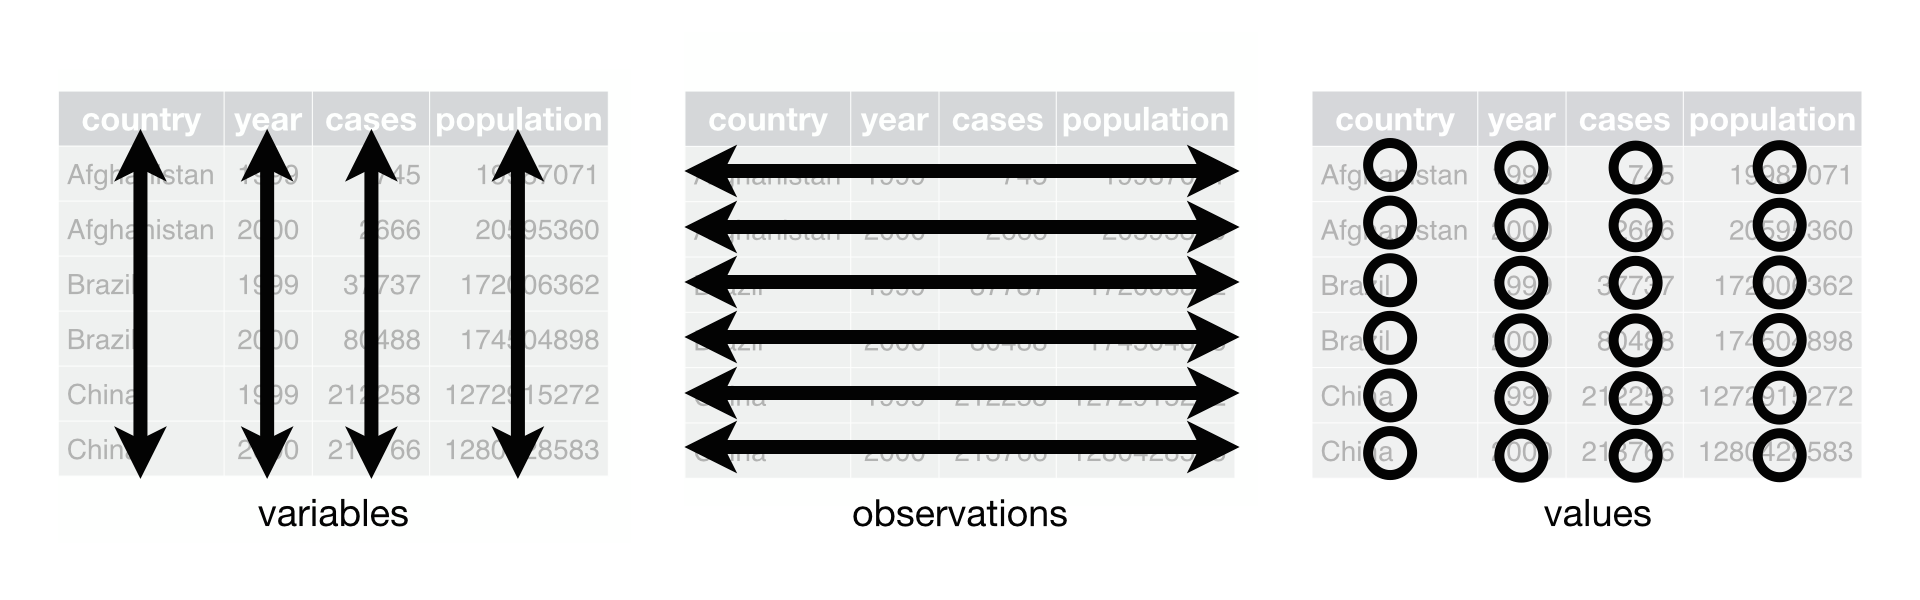
\includegraphics[width=1\linewidth]{images/tidy/tidy-1} 

}

\caption{Following three rules makes a dataset tidy: variables are in columns, observations are in rows, and values are in cells.}\label{fig:tidy-structure}
\end{figure}

These three rules are interrelated because it's impossible to only
satisfy two of the three.

Why ensure that your data is tidy? There are two main advantages:

\begin{enumerate}
\def\labelenumi{\arabic{enumi}.}
\item
  There's a general advantage to picking one consistent way of storing
  data. If you have a consistent data structure, it's easier to learn
  the tools that work with it because they have an underlying
  uniformity.
\item
  There's a specific advantage to placing variables in columns because
  it allows R's vectorized nature to shine. As you learned in
  \protect\hyperlink{mutate-funs}{mutate} and
  \protect\hyperlink{summary-funs}{summary functions}, most built-in R
  functions work with vectors of values. That makes transforming tidy
  data feel particularly natural.
\end{enumerate}

dplyr, ggplot2, and all the other packages in the tidyverse are designed
to work with tidy data.

\section{Example}\label{example-1}

You can represent the same underlying data in multiple ways. The example
below shows the same data organised in four different ways. Each dataset
shows the same values of four variables \emph{country}, \emph{year},
\emph{population}, and \emph{cases}, but each dataset organizes the
values in a different way.

\begin{Shaded}
\begin{Highlighting}[]
\NormalTok{table1}
\CommentTok{#> # A tibble: 6 x 4}
\CommentTok{#>   country      year  cases population}
\CommentTok{#>   <chr>       <int>  <int>      <int>}
\CommentTok{#> 1 Afghanistan  1999    745   19987071}
\CommentTok{#> 2 Afghanistan  2000   2666   20595360}
\CommentTok{#> 3 Brazil       1999  37737  172006362}
\CommentTok{#> 4 Brazil       2000  80488  174504898}
\CommentTok{#> 5 China        1999 212258 1272915272}
\CommentTok{#> 6 China        2000 213766 1280428583}
\NormalTok{table2}
\CommentTok{#> # A tibble: 12 x 4}
\CommentTok{#>   country      year type           count}
\CommentTok{#>   <chr>       <int> <chr>          <int>}
\CommentTok{#> 1 Afghanistan  1999 cases            745}
\CommentTok{#> 2 Afghanistan  1999 population  19987071}
\CommentTok{#> 3 Afghanistan  2000 cases           2666}
\CommentTok{#> 4 Afghanistan  2000 population  20595360}
\CommentTok{#> 5 Brazil       1999 cases          37737}
\CommentTok{#> 6 Brazil       1999 population 172006362}
\CommentTok{#> # ... with 6 more rows}
\NormalTok{table3}
\CommentTok{#> # A tibble: 6 x 3}
\CommentTok{#>   country      year rate             }
\CommentTok{#> * <chr>       <int> <chr>            }
\CommentTok{#> 1 Afghanistan  1999 745/19987071     }
\CommentTok{#> 2 Afghanistan  2000 2666/20595360    }
\CommentTok{#> 3 Brazil       1999 37737/172006362  }
\CommentTok{#> 4 Brazil       2000 80488/174504898  }
\CommentTok{#> 5 China        1999 212258/1272915272}
\CommentTok{#> 6 China        2000 213766/1280428583}

\CommentTok{# Spread across two tibbles}
\NormalTok{table4a  }\CommentTok{# cases}
\CommentTok{#> # A tibble: 3 x 3}
\CommentTok{#>   country     `1999` `2000`}
\CommentTok{#> * <chr>        <int>  <int>}
\CommentTok{#> 1 Afghanistan    745   2666}
\CommentTok{#> 2 Brazil       37737  80488}
\CommentTok{#> 3 China       212258 213766}
\NormalTok{table4b  }\CommentTok{# population}
\CommentTok{#> # A tibble: 3 x 3}
\CommentTok{#>   country         `1999`     `2000`}
\CommentTok{#> * <chr>            <int>      <int>}
\CommentTok{#> 1 Afghanistan   19987071   20595360}
\CommentTok{#> 2 Brazil       172006362  174504898}
\CommentTok{#> 3 China       1272915272 1280428583}
\end{Highlighting}
\end{Shaded}

These are all representations of the same underlying data, but they are
not equally easy to use. One dataset, the tidy dataset, will be much
easier to work with inside the tidyverse.

Which dataset is tidy? Why aren't the other datasets considered tidy?

\BeginKnitrBlock{rmdtip}
How would you calculate the rate per 10,000 population for each data
set? How would you compute the cases per year? How would you visualize
the changes over time?
\EndKnitrBlock{rmdtip}

\section{Spreading and gathering}\label{spreading-and-gathering}

The principles of tidy data seem so obvious that you might wonder if
you'll ever encounter a dataset that isn't tidy. Unfortunately, however,
most data that you will encounter will be untidy. There are two main
reasons:

\begin{enumerate}
\def\labelenumi{\arabic{enumi}.}
\item
  Most people aren't familiar with the principles of tidy data, and it's
  hard to derive them yourself unless you spend a \emph{lot} of time
  working with data.
\item
  Data is often organised to facilitate some use other than analysis.
  For example, data is often organised to make entry as easy as
  possible.
\item
  How to efficiently store, analyze, and present data are \emph{usually}
  three different data formats.
\end{enumerate}

This means for most real analyses, you'll need to do some tidying /
untidying. The first step is always to figure out what the variables and
observations are. Sometimes this is easy; other times it can be a bit
more difficult. The second step is to resolve one of two common
problems:

\begin{enumerate}
\def\labelenumi{\arabic{enumi}.}
\item
  One variable might be spread across multiple columns.
\item
  One observation might be scattered across multiple rows.
\end{enumerate}

Typically a dataset will only suffer from one of these problems; it'll
only suffer from both if you're really unlucky! To fix these problems,
you'll need the two most important functions in tidyr: \texttt{gather()}
and \texttt{spread()}.

\subsection{Gathering}\label{gathering}

A common problem is a dataset where some of the column names are not
names of variables, but \emph{values} of a variable. Take
\texttt{table4a}: the column names \texttt{1999} and \texttt{2000}
represent values of the \texttt{year} variable, and each row represents
two observations, not one.

\begin{Shaded}
\begin{Highlighting}[]
\NormalTok{table4a}
\CommentTok{#> # A tibble: 3 x 3}
\CommentTok{#>   country     `1999` `2000`}
\CommentTok{#> * <chr>        <int>  <int>}
\CommentTok{#> 1 Afghanistan    745   2666}
\CommentTok{#> 2 Brazil       37737  80488}
\CommentTok{#> 3 China       212258 213766}
\end{Highlighting}
\end{Shaded}

\begin{figure}

{\centering 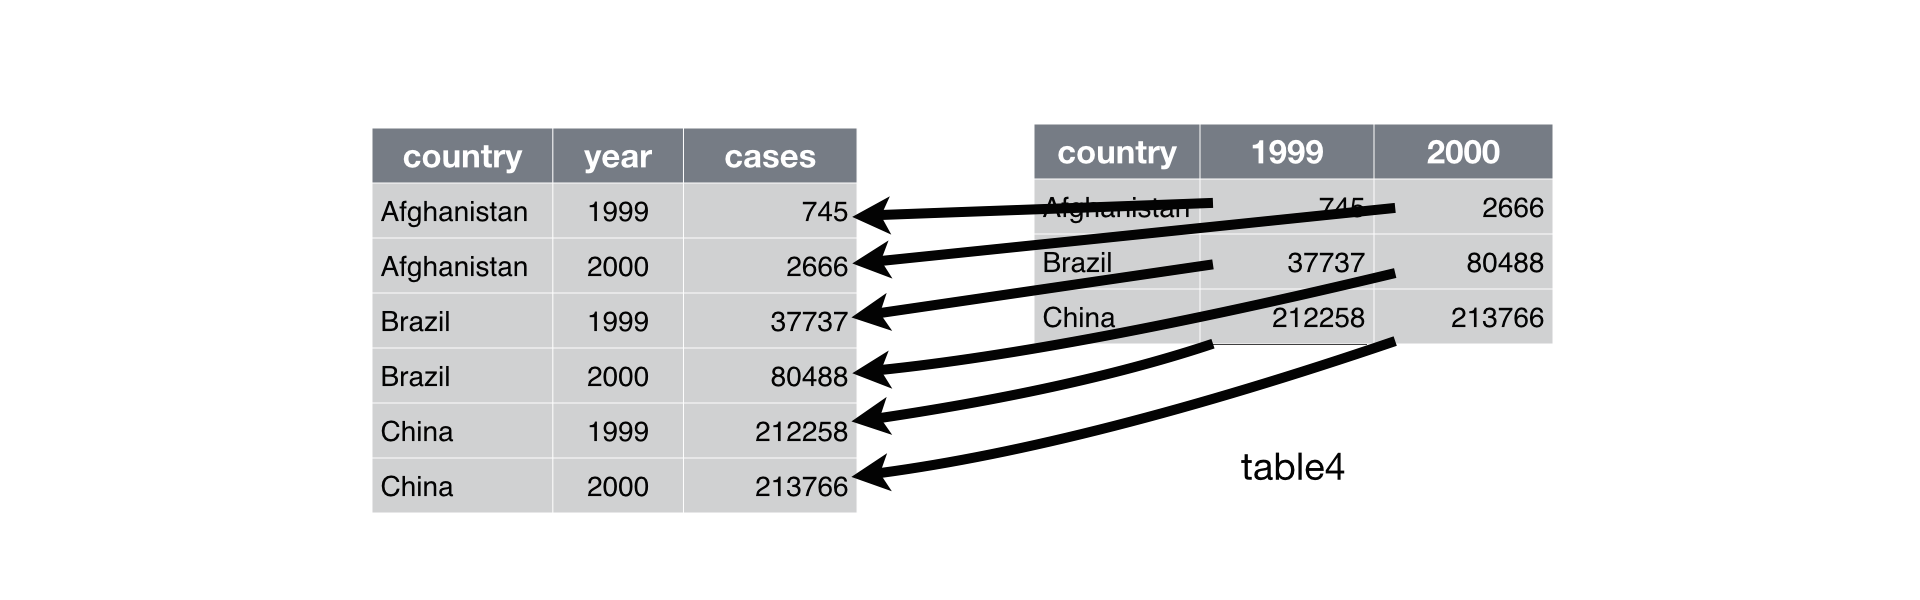
\includegraphics[width=1\linewidth]{images/tidy/tidy-9} 

}

\caption{Gathering `table4` into a tidy form.}\label{fig:tidy-gather}
\end{figure}

To tidy a dataset like this, we need to \textbf{gather} those columns
into a new pair of variables. To describe that operation we need three
parameters:

\begin{itemize}
\item
  The name of the variable whose values form the column names. This is
  the \texttt{key}, and here it is \texttt{year}.
\item
  The name of the variable whose values are spread over the cells. That
  is the \texttt{value}, and here it's the number of \texttt{cases}.
\item
  The set of columns that represent values, not variables. In this
  example, those are the columns \texttt{1999} and \texttt{2000}.
\end{itemize}

Together those parameters generate the call to \texttt{gather()}:

\begin{Shaded}
\begin{Highlighting}[]
\NormalTok{table4a }\OperatorTok\StringTok{ }
\StringTok{  }\KeywordTok{gather}\NormalTok{(}\DataTypeTok{key =} \StringTok{"year"}\NormalTok{, }\DataTypeTok{value =} \StringTok{"cases"}\NormalTok{, }\StringTok{`}\DataTypeTok{1999}\StringTok{`}\NormalTok{, }\StringTok{`}\DataTypeTok{2000}\StringTok{`}\NormalTok{)}
\CommentTok{#> # A tibble: 6 x 3}
\CommentTok{#>   country     year   cases}
\CommentTok{#>   <chr>       <chr>  <int>}
\CommentTok{#> 1 Afghanistan 1999     745}
\CommentTok{#> 2 Brazil      1999   37737}
\CommentTok{#> 3 China       1999  212258}
\CommentTok{#> 4 Afghanistan 2000    2666}
\CommentTok{#> 5 Brazil      2000   80488}
\CommentTok{#> 6 China       2000  213766}
\end{Highlighting}
\end{Shaded}

\BeginKnitrBlock{rmdimportant}
Note that ``1999'' and ``2000'' are non-syntactic names (because they
don't start with a letter) so we have to surround them in backticks. To
refresh your memory of the other ways to select columns, see
\protect\hyperlink{select}{select}.
\EndKnitrBlock{rmdimportant}

In the final result, the gathered columns are dropped, and we get new
\texttt{key} and \texttt{value} columns. Otherwise, the relationships
between the original variables are preserved. Visually, this is shown in
Figure \ref{fig:tidy-gather}. We can use \texttt{gather()} to tidy
\texttt{table4b} in a similar fashion. The only difference is the
variable stored in the cell values.

To combine the tidied versions of \texttt{table4a} and \texttt{table4b}
into a single tibble, we need to use \texttt{dplyr::left\_join()}, which
you'll learn about in {[}relational data{]}.

\begin{Shaded}
\begin{Highlighting}[]
\NormalTok{tidy4a <-}\StringTok{ }\NormalTok{table4a }\OperatorTok\StringTok{ }
\StringTok{  }\KeywordTok{gather}\NormalTok{(}\DataTypeTok{key =} \StringTok{"year"}\NormalTok{, }\DataTypeTok{value =} \StringTok{"cases"}\NormalTok{, }\StringTok{`}\DataTypeTok{1999}\StringTok{`}\NormalTok{, }\StringTok{`}\DataTypeTok{2000}\StringTok{`}\NormalTok{)}
\NormalTok{tidy4b <-}\StringTok{ }\NormalTok{table4b }\OperatorTok\StringTok{ }
\StringTok{  }\KeywordTok{gather}\NormalTok{(}\DataTypeTok{key =} \StringTok{"year"}\NormalTok{, }\DataTypeTok{value =} \StringTok{"population"}\NormalTok{, }\StringTok{`}\DataTypeTok{1999}\StringTok{`}\NormalTok{, }\StringTok{`}\DataTypeTok{2000}\StringTok{`}\NormalTok{)}
\KeywordTok{left_join}\NormalTok{(tidy4a, tidy4b)}
\CommentTok{#> Joining, by = c("country", "year")}
\CommentTok{#> # A tibble: 6 x 4}
\CommentTok{#>   country     year   cases population}
\CommentTok{#>   <chr>       <chr>  <int>      <int>}
\CommentTok{#> 1 Afghanistan 1999     745   19987071}
\CommentTok{#> 2 Brazil      1999   37737  172006362}
\CommentTok{#> 3 China       1999  212258 1272915272}
\CommentTok{#> 4 Afghanistan 2000    2666   20595360}
\CommentTok{#> 5 Brazil      2000   80488  174504898}
\CommentTok{#> 6 China       2000  213766 1280428583}
\end{Highlighting}
\end{Shaded}

\subsection{Spreading}\label{spreading}

Spreading is the opposite of gathering. You use it when an observation
is scattered across multiple rows. For example, take \texttt{table2}: an
observation is a country in a year, but each observation is spread
across two rows.

\begin{Shaded}
\begin{Highlighting}[]
\NormalTok{table2}
\CommentTok{#> # A tibble: 12 x 4}
\CommentTok{#>   country      year type           count}
\CommentTok{#>   <chr>       <int> <chr>          <int>}
\CommentTok{#> 1 Afghanistan  1999 cases            745}
\CommentTok{#> 2 Afghanistan  1999 population  19987071}
\CommentTok{#> 3 Afghanistan  2000 cases           2666}
\CommentTok{#> 4 Afghanistan  2000 population  20595360}
\CommentTok{#> 5 Brazil       1999 cases          37737}
\CommentTok{#> 6 Brazil       1999 population 172006362}
\CommentTok{#> # ... with 6 more rows}
\end{Highlighting}
\end{Shaded}

\begin{figure}

{\centering 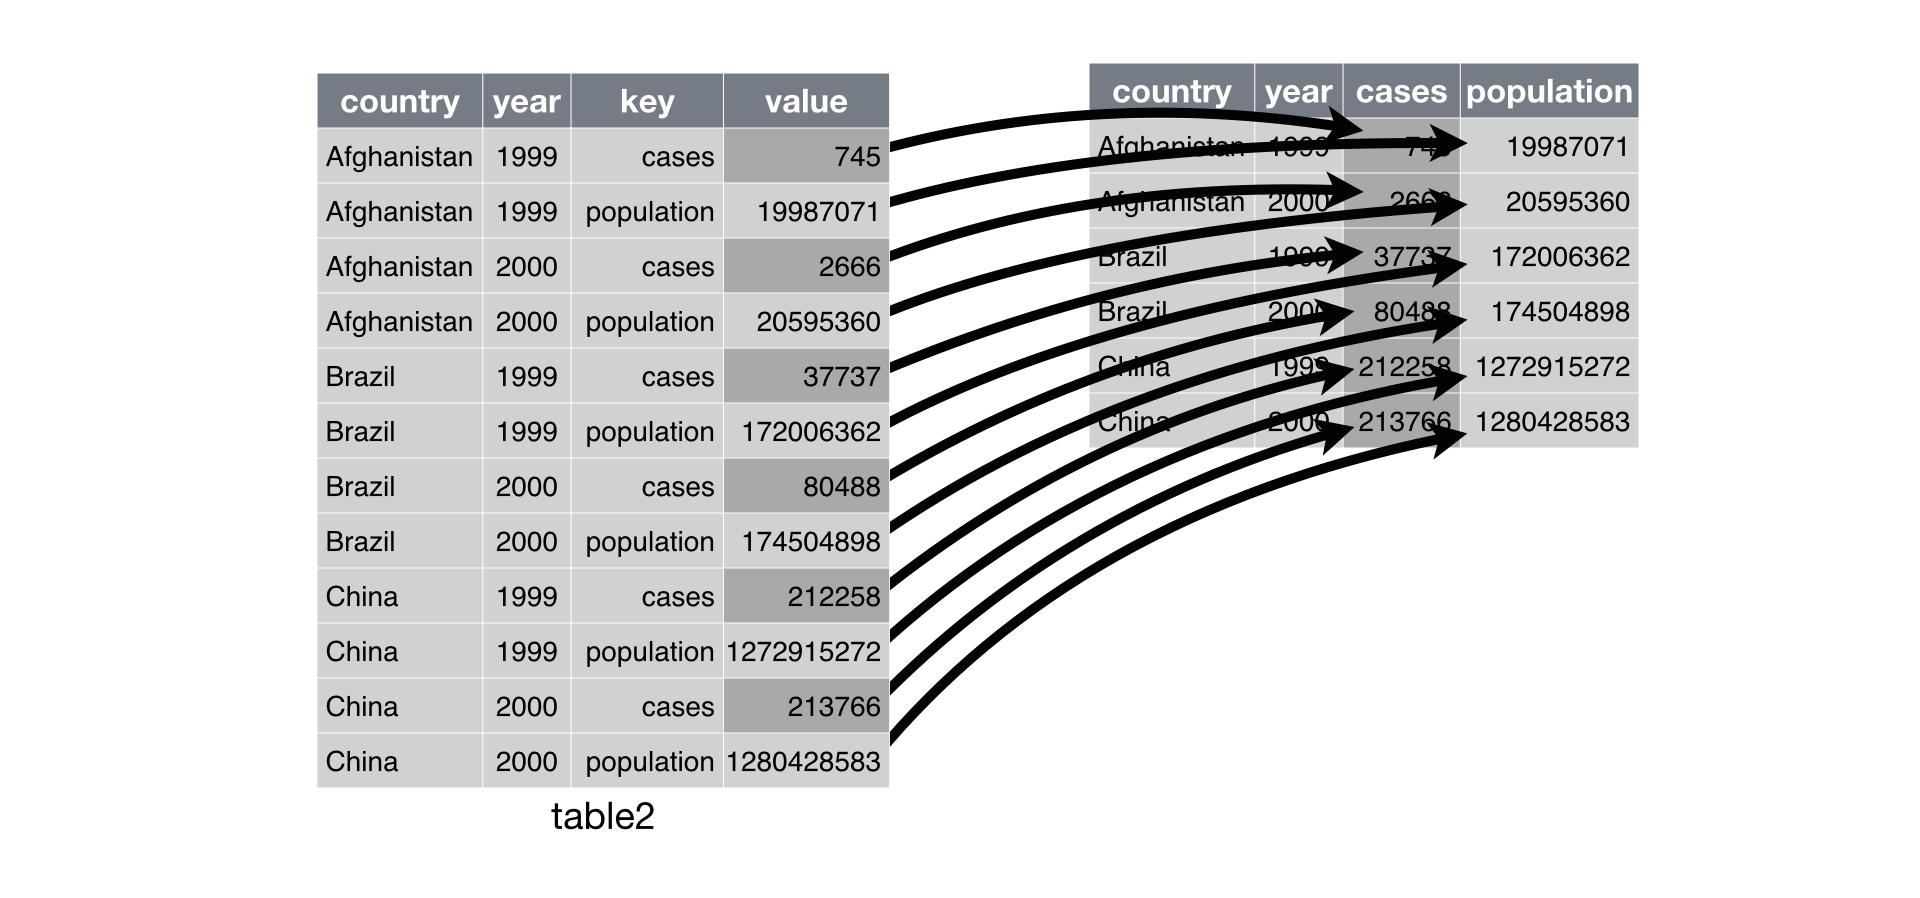
\includegraphics[width=1\linewidth]{images/tidy/tidy-8} 

}

\caption{Spreading `table2` makes it tidy}\label{fig:tidy-spread}
\end{figure}

To tidy this up, we first analyse the representation in similar way to
\texttt{gather()}. This time, however, we only need two parameters:

\begin{itemize}
\item
  The column that contains variable names, the \texttt{key} column.
  Here, it's \texttt{type}.
\item
  The column that contains values from multiple variables, the
  \texttt{value} column. Here it's \texttt{count}.
\end{itemize}

Once we've figured that out, we can use \texttt{spread()}, as shown
programmatically below, and visually in Figure \ref{fig:tidy-spread}.

\begin{Shaded}
\begin{Highlighting}[]
\NormalTok{table2 }\OperatorTok
\StringTok{    }\KeywordTok{spread}\NormalTok{(}\DataTypeTok{key =}\NormalTok{ type, }\DataTypeTok{value =}\NormalTok{ count)}
\CommentTok{#> # A tibble: 6 x 4}
\CommentTok{#>   country      year  cases population}
\CommentTok{#>   <chr>       <int>  <int>      <int>}
\CommentTok{#> 1 Afghanistan  1999    745   19987071}
\CommentTok{#> 2 Afghanistan  2000   2666   20595360}
\CommentTok{#> 3 Brazil       1999  37737  172006362}
\CommentTok{#> 4 Brazil       2000  80488  174504898}
\CommentTok{#> 5 China        1999 212258 1272915272}
\CommentTok{#> 6 China        2000 213766 1280428583}
\end{Highlighting}
\end{Shaded}

\begin{rmdnote}
As you might have guessed from the common \texttt{key} and
\texttt{value} arguments, \texttt{spread()} and \texttt{gather()} are
complements. \texttt{gather()} makes wide tables narrower and longer;
\texttt{spread()} makes long tables shorter and wider.
\end{rmdnote}

\section{Separating and uniting}\label{separating-and-uniting}

So far you've learned how to tidy \texttt{table2} and \texttt{table4},
but not \texttt{table3}. \texttt{table3} has a different problem: we
have one column (\texttt{rate}) that contains two variables
(\texttt{cases} and \texttt{population}). To fix this problem, we'll
need the \texttt{separate()} function. You'll also learn about the
complement of \texttt{separate()}: \texttt{unite()}, which you use if a
single variable is spread across multiple columns.

\subsection{Separate}\label{separate}

\texttt{separate()} pulls apart one column into multiple columns, by
splitting wherever a separator character appears. Take \texttt{table3}:

\begin{Shaded}
\begin{Highlighting}[]
\NormalTok{table3}
\CommentTok{#> # A tibble: 6 x 3}
\CommentTok{#>   country      year rate             }
\CommentTok{#> * <chr>       <int> <chr>            }
\CommentTok{#> 1 Afghanistan  1999 745/19987071     }
\CommentTok{#> 2 Afghanistan  2000 2666/20595360    }
\CommentTok{#> 3 Brazil       1999 37737/172006362  }
\CommentTok{#> 4 Brazil       2000 80488/174504898  }
\CommentTok{#> 5 China        1999 212258/1272915272}
\CommentTok{#> 6 China        2000 213766/1280428583}
\end{Highlighting}
\end{Shaded}

\begin{figure}

{\centering 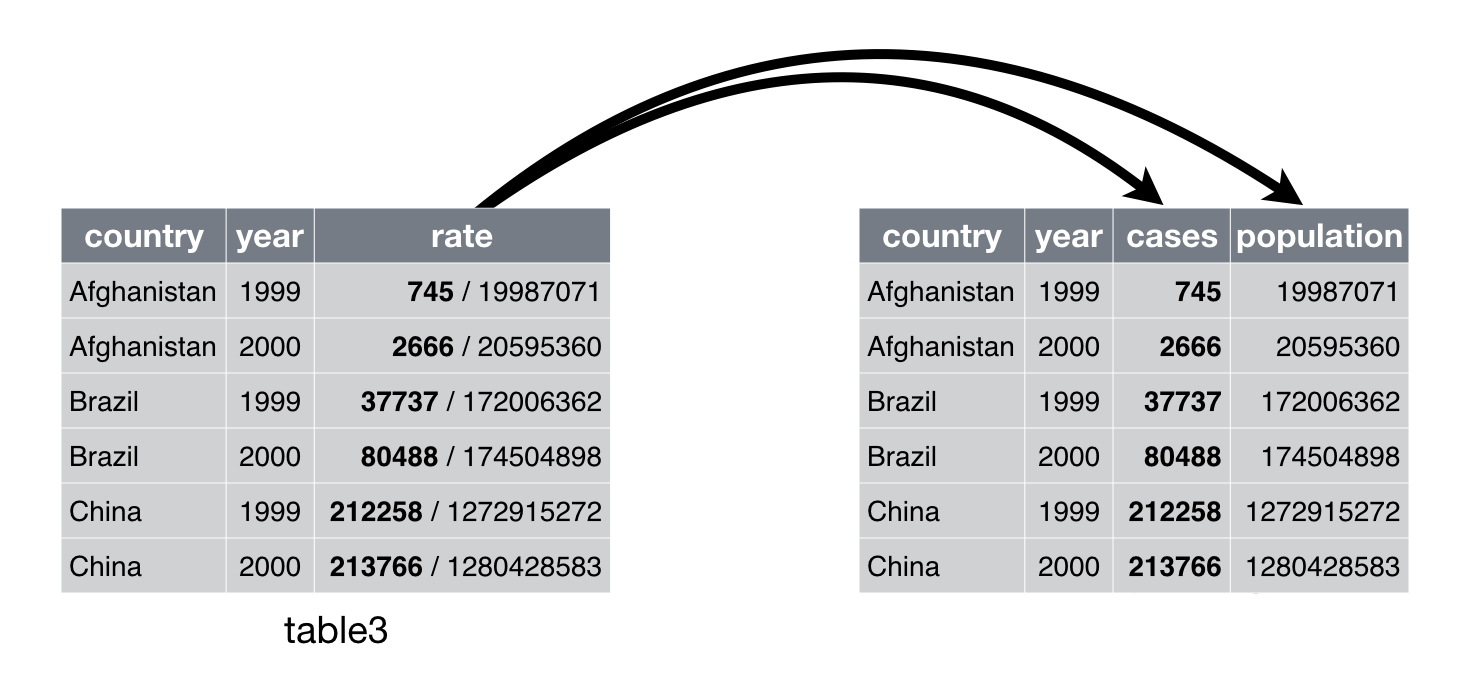
\includegraphics[width=0.75\linewidth]{images/tidy/tidy-17} 

}

\caption{Separating `table3` makes it tidy}\label{fig:tidy-separate}
\end{figure}

The \texttt{rate} column contains both \texttt{cases} and
\texttt{population} variables, and we need to split it into two
variables. \texttt{separate()} takes the name of the column to separate,
and the names of the columns to separate into, as shown in Figure
\ref{fig:tidy-separate} and the code below.

\begin{Shaded}
\begin{Highlighting}[]
\NormalTok{table3 }\OperatorTok\StringTok{ }
\StringTok{  }\KeywordTok{separate}\NormalTok{(rate, }\DataTypeTok{into =} \KeywordTok{c}\NormalTok{(}\StringTok{"cases"}\NormalTok{, }\StringTok{"population"}\NormalTok{))}
\CommentTok{#> # A tibble: 6 x 4}
\CommentTok{#>   country      year cases  population}
\CommentTok{#> * <chr>       <int> <chr>  <chr>     }
\CommentTok{#> 1 Afghanistan  1999 745    19987071  }
\CommentTok{#> 2 Afghanistan  2000 2666   20595360  }
\CommentTok{#> 3 Brazil       1999 37737  172006362 }
\CommentTok{#> 4 Brazil       2000 80488  174504898 }
\CommentTok{#> 5 China        1999 212258 1272915272}
\CommentTok{#> 6 China        2000 213766 1280428583}
\end{Highlighting}
\end{Shaded}

\BeginKnitrBlock{rmdimportant}
By default, \texttt{separate()} will split values wherever it sees a
non-alphanumeric character (i.e.~a character that isn't a number or
letter). For example, in the code above, \texttt{separate()} split the
values of \texttt{rate} at the forward slash characters. If you wish to
use a specific character to separate a column, you can pass the
character to the \texttt{sep} argument of \texttt{separate()}. Formally,
\texttt{sep} is a regular expression, which we learn more about in
{[}strings{]}.
\EndKnitrBlock{rmdimportant}

Look carefully at the column types: you'll notice that \texttt{cases}
and \texttt{population} are character columns. This is the default
behavior in \texttt{separate()}: it leaves the type of the column as is.
Here, however, it's not very useful as those really are numbers. We can
ask \texttt{separate()} to try and convert to better types using
\texttt{convert\ =\ TRUE}:

\begin{Shaded}
\begin{Highlighting}[]
\NormalTok{table3 }\OperatorTok\StringTok{ }
\StringTok{  }\KeywordTok{separate}\NormalTok{(rate, }\DataTypeTok{into =} \KeywordTok{c}\NormalTok{(}\StringTok{"cases"}\NormalTok{, }\StringTok{"population"}\NormalTok{), }\DataTypeTok{convert =} \OtherTok{TRUE}\NormalTok{)}
\CommentTok{#> # A tibble: 6 x 4}
\CommentTok{#>   country      year  cases population}
\CommentTok{#> * <chr>       <int>  <int>      <int>}
\CommentTok{#> 1 Afghanistan  1999    745   19987071}
\CommentTok{#> 2 Afghanistan  2000   2666   20595360}
\CommentTok{#> 3 Brazil       1999  37737  172006362}
\CommentTok{#> 4 Brazil       2000  80488  174504898}
\CommentTok{#> 5 China        1999 212258 1272915272}
\CommentTok{#> 6 China        2000 213766 1280428583}
\end{Highlighting}
\end{Shaded}

You can also pass a vector of integers to \texttt{sep}.
\texttt{separate()} will interpret the integers as positions to split
at. Positive values start at 1 on the far-left of the strings; negative
value start at -1 on the far-right of the strings. When using integers
to separate strings, the length of \texttt{sep} should be one less than
the number of names in \texttt{into}.

You can use this arrangement to separate the last two digits of each
year. This make this data less tidy, but is useful in other cases, as
you'll see in a little bit.

\begin{Shaded}
\begin{Highlighting}[]
\NormalTok{table3 }\OperatorTok\StringTok{ }
\StringTok{  }\KeywordTok{separate}\NormalTok{(year, }\DataTypeTok{into =} \KeywordTok{c}\NormalTok{(}\StringTok{"century"}\NormalTok{, }\StringTok{"year"}\NormalTok{), }\DataTypeTok{sep =} \DecValTok{2}\NormalTok{)}
\CommentTok{#> # A tibble: 6 x 4}
\CommentTok{#>   country     century year  rate             }
\CommentTok{#> * <chr>       <chr>   <chr> <chr>            }
\CommentTok{#> 1 Afghanistan 19      99    745/19987071     }
\CommentTok{#> 2 Afghanistan 20      00    2666/20595360    }
\CommentTok{#> 3 Brazil      19      99    37737/172006362  }
\CommentTok{#> 4 Brazil      20      00    80488/174504898  }
\CommentTok{#> 5 China       19      99    212258/1272915272}
\CommentTok{#> 6 China       20      00    213766/1280428583}
\end{Highlighting}
\end{Shaded}

\subsection{Unite}\label{unite}

\texttt{unite()} is the inverse of \texttt{separate()}: it combines
multiple columns into a single column. You'll need it much less
frequently than \texttt{separate()}, but it's still a useful tool to
have in your back pocket.

\begin{figure}

{\centering 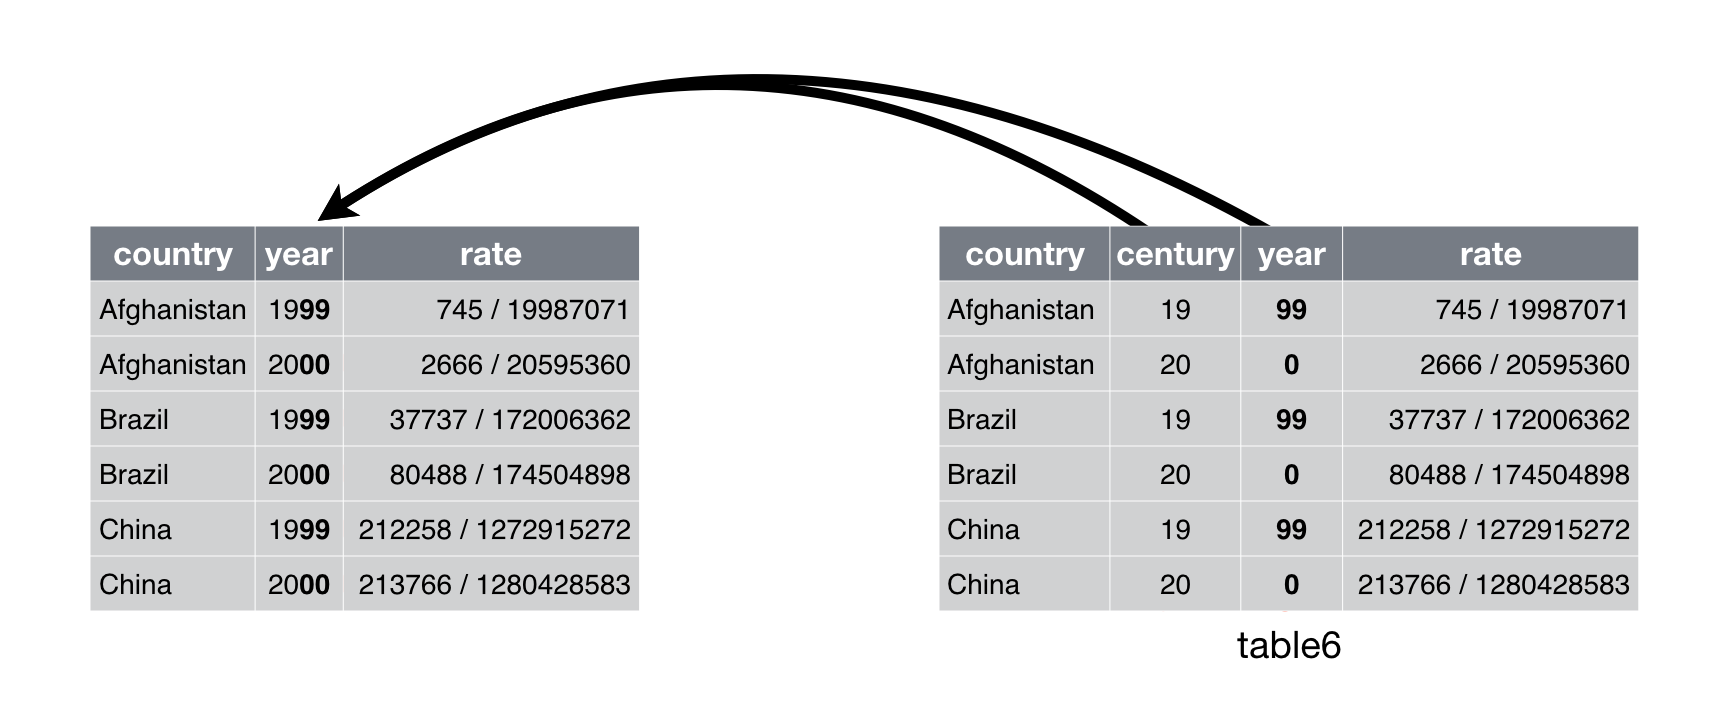
\includegraphics[width=0.75\linewidth]{images/tidy/tidy-18} 

}

\caption{Uniting `table5` makes it tidy}\label{fig:tidy-unite}
\end{figure}

We can use \texttt{unite()} to rejoin the \emph{century} and \emph{year}
columns that we created in the last example. That data is saved as
\texttt{tidyr::table5}. \texttt{unite()} takes a data frame, the name of
the new variable to create, and a set of columns to combine, again
specified in \texttt{dplyr::select()} style:

\begin{Shaded}
\begin{Highlighting}[]
\NormalTok{table5 }\OperatorTok\StringTok{ }
\StringTok{  }\KeywordTok{unite}\NormalTok{(new, century, year)}
\CommentTok{#> # A tibble: 6 x 3}
\CommentTok{#>   country     new   rate             }
\CommentTok{#>   <chr>       <chr> <chr>            }
\CommentTok{#> 1 Afghanistan 19_99 745/19987071     }
\CommentTok{#> 2 Afghanistan 20_00 2666/20595360    }
\CommentTok{#> 3 Brazil      19_99 37737/172006362  }
\CommentTok{#> 4 Brazil      20_00 80488/174504898  }
\CommentTok{#> 5 China       19_99 212258/1272915272}
\CommentTok{#> 6 China       20_00 213766/1280428583}
\end{Highlighting}
\end{Shaded}

In this case we also need to use the \texttt{sep} argument. The default
will place an underscore (\texttt{\_}) between the values from different
columns. Here we don't want any separator so we use \texttt{""}:

\begin{Shaded}
\begin{Highlighting}[]
\NormalTok{table5 }\OperatorTok\StringTok{ }
\StringTok{  }\KeywordTok{unite}\NormalTok{(new, century, year, }\DataTypeTok{sep =} \StringTok{""}\NormalTok{)}
\CommentTok{#> # A tibble: 6 x 3}
\CommentTok{#>   country     new   rate             }
\CommentTok{#>   <chr>       <chr> <chr>            }
\CommentTok{#> 1 Afghanistan 1999  745/19987071     }
\CommentTok{#> 2 Afghanistan 2000  2666/20595360    }
\CommentTok{#> 3 Brazil      1999  37737/172006362  }
\CommentTok{#> 4 Brazil      2000  80488/174504898  }
\CommentTok{#> 5 China       1999  212258/1272915272}
\CommentTok{#> 6 China       2000  213766/1280428583}
\end{Highlighting}
\end{Shaded}

\section{Missing values}\label{missing-values}

Changing the representation of a dataset brings up an important subtlety
of missing values. Surprisingly, a value can be missing in one of two
possible ways:

\begin{itemize}
\tightlist
\item
  \textbf{Explicitly}, i.e.~flagged with \texttt{NA}.
\item
  \textbf{Implicitly}, i.e.~simply not present in the data.
\end{itemize}

Let's illustrate this idea with a very simple data set:

\begin{Shaded}
\begin{Highlighting}[]
\NormalTok{mydata <-}\StringTok{ }\KeywordTok{tibble}\NormalTok{(}
  \DataTypeTok{year   =} \KeywordTok{c}\NormalTok{(}\DecValTok{2015}\NormalTok{, }\DecValTok{2015}\NormalTok{, }\DecValTok{2015}\NormalTok{, }\DecValTok{2015}\NormalTok{, }\DecValTok{2016}\NormalTok{, }\DecValTok{2016}\NormalTok{, }\DecValTok{2016}\NormalTok{),}
  \DataTypeTok{qtr    =} \KeywordTok{c}\NormalTok{(   }\DecValTok{1}\NormalTok{,    }\DecValTok{2}\NormalTok{,    }\DecValTok{3}\NormalTok{,    }\DecValTok{4}\NormalTok{,    }\DecValTok{2}\NormalTok{,    }\DecValTok{3}\NormalTok{,    }\DecValTok{4}\NormalTok{),}
  \DataTypeTok{rate   =} \KeywordTok{c}\NormalTok{(}\FloatTok{1.88}\NormalTok{, }\FloatTok{0.59}\NormalTok{, }\FloatTok{0.35}\NormalTok{,   }\OtherTok{NA}\NormalTok{, }\FloatTok{0.92}\NormalTok{, }\FloatTok{0.17}\NormalTok{, }\FloatTok{2.66}\NormalTok{)}
\NormalTok{)}

\NormalTok{mydata}
\CommentTok{#> # A tibble: 7 x 3}
\CommentTok{#>    year   qtr  rate}
\CommentTok{#>   <dbl> <dbl> <dbl>}
\CommentTok{#> 1  2015     1  1.88}
\CommentTok{#> 2  2015     2  0.59}
\CommentTok{#> 3  2015     3  0.35}
\CommentTok{#> 4  2015     4 NA   }
\CommentTok{#> 5  2016     2  0.92}
\CommentTok{#> 6  2016     3  0.17}
\CommentTok{#> # ... with 1 more row}
\end{Highlighting}
\end{Shaded}

There are two missing values in this dataset:

\begin{itemize}
\item
  The rate for the fourth quarter of 2015 is explicitly missing, because
  the cell where its value should be instead contains \texttt{NA}.
\item
  The rate for the first quarter of 2016 is implicitly missing, because
  it simply does not appear in the dataset.
\end{itemize}

The way that a dataset is represented can make implicit values explicit.
For example, we can make the implicit missing value explicit by putting
years in the columns:

\begin{Shaded}
\begin{Highlighting}[]
\NormalTok{mydata }\OperatorTok\StringTok{ }
\StringTok{  }\KeywordTok{spread}\NormalTok{(year, rate)}
\CommentTok{#> # A tibble: 4 x 3}
\CommentTok{#>     qtr `2015` `2016`}
\CommentTok{#>   <dbl>  <dbl>  <dbl>}
\CommentTok{#> 1     1   1.88  NA   }
\CommentTok{#> 2     2   0.59   0.92}
\CommentTok{#> 3     3   0.35   0.17}
\CommentTok{#> 4     4  NA      2.66}
\end{Highlighting}
\end{Shaded}

Because these explicit missing values may not be important in other
representations of the data, you can set \texttt{na.rm\ =\ TRUE} in
\texttt{gather()} to turn explicit missing values implicit:

\begin{Shaded}
\begin{Highlighting}[]
\NormalTok{mydata }\OperatorTok\StringTok{ }
\StringTok{  }\KeywordTok{spread}\NormalTok{(year, rate) }\OperatorTok\StringTok{ }
\StringTok{  }\KeywordTok{gather}\NormalTok{(year, rate, }\StringTok{`}\DataTypeTok{2015}\StringTok{`}\OperatorTok{:}\StringTok{`}\DataTypeTok{2016}\StringTok{`}\NormalTok{, }\DataTypeTok{na.rm =} \OtherTok{TRUE}\NormalTok{)}
\CommentTok{#> # A tibble: 6 x 3}
\CommentTok{#>     qtr year   rate}
\CommentTok{#> * <dbl> <chr> <dbl>}
\CommentTok{#> 1     1 2015   1.88}
\CommentTok{#> 2     2 2015   0.59}
\CommentTok{#> 3     3 2015   0.35}
\CommentTok{#> 4     2 2016   0.92}
\CommentTok{#> 5     3 2016   0.17}
\CommentTok{#> 6     4 2016   2.66}
\end{Highlighting}
\end{Shaded}

Another important tool for making missing values explicit in tidy data
is \texttt{complete()}:

\begin{Shaded}
\begin{Highlighting}[]
\NormalTok{mydata }\OperatorTok\StringTok{ }
\StringTok{  }\KeywordTok{complete}\NormalTok{(year, qtr)}
\CommentTok{#> # A tibble: 8 x 3}
\CommentTok{#>    year   qtr  rate}
\CommentTok{#>   <dbl> <dbl> <dbl>}
\CommentTok{#> 1  2015     1  1.88}
\CommentTok{#> 2  2015     2  0.59}
\CommentTok{#> 3  2015     3  0.35}
\CommentTok{#> 4  2015     4 NA   }
\CommentTok{#> 5  2016     1 NA   }
\CommentTok{#> 6  2016     2  0.92}
\CommentTok{#> # ... with 2 more rows}
\end{Highlighting}
\end{Shaded}

\texttt{complete()} takes a set of columns, and finds all unique
combinations. It then ensures the original dataset contains all those
values, filling in explicit \texttt{NA}s where necessary.

\BeginKnitrBlock{rmdwarning}
It is also possible that you have such incomplete data that
\texttt{complete()} does not have all the data needed for complete
cases. Imagine in the above example if the year 2016 data wat instead
complete missing but you had 2017 data. In this case a different
technique would need to be used. A common solution to this problem is to
use \texttt{crossing()} to make the compete cases then ``join'' the data
set to the complete cases.
\EndKnitrBlock{rmdwarning}

There's one other important tool that you should know for working with
missing values. Sometimes when a data source has primarily been used for
data entry (tables from \emph{Excel}, \emph{pdf}, and \emph{Word}),
missing values indicate that the previous value should be carried
forward:

\begin{Shaded}
\begin{Highlighting}[]
\NormalTok{treatment <-}\StringTok{ }\KeywordTok{tribble}\NormalTok{(}
  \OperatorTok{~}\StringTok{ }\NormalTok{person,           }\OperatorTok{~}\StringTok{ }\NormalTok{treatment, }\OperatorTok{~}\NormalTok{response,}
  \StringTok{"Derrick Whitmore"}\NormalTok{, }\DecValTok{1}\NormalTok{,           }\DecValTok{7}\NormalTok{,}
  \OtherTok{NA}\NormalTok{,                 }\DecValTok{2}\NormalTok{,           }\DecValTok{10}\NormalTok{,}
  \OtherTok{NA}\NormalTok{,                 }\DecValTok{3}\NormalTok{,           }\DecValTok{9}\NormalTok{,}
  \StringTok{"Katherine Burke"}\NormalTok{,  }\DecValTok{1}\NormalTok{,           }\DecValTok{4}
\NormalTok{)}

\NormalTok{treatment}
\CommentTok{#> # A tibble: 4 x 3}
\CommentTok{#>   person           treatment response}
\CommentTok{#>   <chr>                <dbl>    <dbl>}
\CommentTok{#> 1 Derrick Whitmore         1        7}
\CommentTok{#> 2 <NA>                     2       10}
\CommentTok{#> 3 <NA>                     3        9}
\CommentTok{#> 4 Katherine Burke          1        4}
\end{Highlighting}
\end{Shaded}

You can fill in these missing values with \texttt{fill()}. It takes a
set of columns where you want missing values to be replaced by the most
recent non-missing value (sometimes called last observation carried
forward).

\begin{Shaded}
\begin{Highlighting}[]
\NormalTok{treatment }\OperatorTok\StringTok{ }
\StringTok{  }\KeywordTok{fill}\NormalTok{(person)}
\CommentTok{#> # A tibble: 4 x 3}
\CommentTok{#>   person           treatment response}
\CommentTok{#>   <chr>                <dbl>    <dbl>}
\CommentTok{#> 1 Derrick Whitmore         1        7}
\CommentTok{#> 2 Derrick Whitmore         2       10}
\CommentTok{#> 3 Derrick Whitmore         3        9}
\CommentTok{#> 4 Katherine Burke          1        4}
\end{Highlighting}
\end{Shaded}

\section{Non-tidy data}\label{non-tidy-data}

Before we continue on to other topics, it's worth talking briefly about
non-tidy data. Earlier in the chapter, I used the pejorative term
``messy'' to refer to non-tidy data. That's an oversimplification: there
are lots of useful and well-founded data structures that are not tidy
data. There are two main reasons to use other data structures:

\begin{itemize}
\item
  Alternative representations may have substantial performance or space
  advantages.
\item
  Specialized fields have evolved their own conventions for storing data
  that may be quite different to the conventions of tidy data.
\end{itemize}

Either of these reasons means you'll need something other than a tibble
(or data frame). If your data does fit naturally into a rectangular
structure composed of observations and variables, I think tidy data
should be your default choice. But there are good reasons to use other
structures; tidy data is not the only way.

If you'd like to learn more about non-tidy data, I'd highly recommend
this thoughtful blog post by Jeff Leek:
\url{http://simplystatistics.org/2016/02/17/non-tidy-data/}

\part{Beyond Basics}\label{part-beyond-basics}

\chapter{Function Basics}\label{function-basics}

\begin{quote}
To understand computations in R, two slogans are helpful:\\
- Everything that exists is an object.\\
- Everything that happens is a function call.

-- John Chambers
\end{quote}

\section{Introduction to Functions}\label{introduction-to-functions}

Functions are an central part of robust R programming and we will spend
a significant amount of time writing functions. Think of functions in
the
\href{https://en.wikipedia.org/wiki/Function_(mathematics)}{mathematical
sense} will make the properties much more apparent than any other
framework.

Functions in R are ``first class objects'', which means that they can be
treated much like any other R object. Importantly,

\begin{itemize}
\item
  Functions can be passed as arguments to other functions. This is very
  handy for the various apply functions, like \texttt{lapply()} and
  \texttt{sapply()}.
\item
  Functions can be nested, so that you can define a function inside of
  another function
\end{itemize}

If you're familiar with common language like C, these features might
appear a bit strange. However, they are really important in R and can be
useful for data analysis.

\begin{itemize}
\tightlist
\item
  Functions are a means of \textbf{abstraction}. A concept/computation
  is encapsulated/isolated from the rest with a function.
\item
  Functions should \textbf{do one thing}, and do it well (compute, or
  plot, or save, \ldots{} not all in one go).
\item
  \textbf{Side effects}: your functions should not have any (unless, of
  course, that is the main point of that function - plotting, write to
  disk, \ldots{}). Functions shouldn't make any changes in any
  environment. The only return their output.
\item
  \textbf{Do not use global variables}. Everything the function needs is
  being passed as an argument. Function must be \textbf{self-contained}.
\item
  Function streamline code and process
\end{itemize}

Advice from the
\href{http://www.burns-stat.com/pages/Tutor/R_inferno.pdf}{R Inferno}:

Make your functions as simple as possible. Simple has many advantages:

\begin{itemize}
\tightlist
\item
  Simple functions are likely to be human efficient: they will be easy
  to understand and to modify.
\item
  Simple functions are likely to be computer efficient.
\item
  Simple functions are less likely to be buggy, and bugs will be easier
  to fix.
\item
  (Perhaps ironically) simple functions may be more general---thinking
  about the heart of the matter often broadens the application.
\end{itemize}

Functions can be

\begin{enumerate}
\def\labelenumi{\arabic{enumi}.}
\tightlist
\item
  Correct.
\item
  An error occurs that is clearly identified.
\item
  An obscure error occurs.
\item
  An incorrect value is returned.
\end{enumerate}

We like \textbf{category 1}. \textbf{Category 2} is the right behavior
if the inputs do not make sense, but not if the inputs are sensible.
\textbf{Category 3} is an unpleasant place for your users, and possibly
for you if the users have access to you. \textbf{Category 4} is by far
the worst place to be - the user has no reason to believe that anything
is wrong. Steer clear of category 4.

\begin{rmdimportant}
Software testing is important, but, in part because it is frustrating
and boring, many of us avoid it. `testthat' is a testing framework for R
that is easy learn and use, and integrates with your existing
`workflow'.
\end{rmdimportant}

\subsection{Your First Function}\label{your-first-function}

All R functions have three parts:

\begin{itemize}
\item
  the \texttt{body()}, the code inside the function.
\item
  the \texttt{formals()}, the list of arguments which controls how you
  can call the function.
\item
  the \texttt{environment()}, the ``map'' of the location of the
  function's variables.
\end{itemize}

When you print a function in R, it shows you these three important
components. If the environment isn't displayed, it means that the
function was created in the global environment.

\begin{Shaded}
\begin{Highlighting}[]
\NormalTok{myadd <-}\StringTok{ }\ControlFlowTok{function}\NormalTok{(x, y) \{}
  \KeywordTok{message}\NormalTok{(}\KeywordTok{paste0}\NormalTok{(}\StringTok{"x = "}\NormalTok{, x, }\StringTok{"}\CharTok{\textbackslash{}n}\StringTok{"}\NormalTok{))}
  \KeywordTok{message}\NormalTok{(}\KeywordTok{paste0}\NormalTok{(}\StringTok{"y = "}\NormalTok{, y, }\StringTok{"}\CharTok{\textbackslash{}n}\StringTok{"}\NormalTok{))}
\NormalTok{  x }\OperatorTok{+}\StringTok{ }\NormalTok{y}
\NormalTok{\}}
\end{Highlighting}
\end{Shaded}

\begin{itemize}
\tightlist
\item
  The body of the function is everything between the \texttt{\{\ \}}.
  Note this does the computation \textbf{AND} returns the result.
\item
  \texttt{x} and \texttt{y} are the arguments to the function.
\item
  the environment this function lives in is the global environment.
  (We'll discuss environments more in the next section.)
\end{itemize}

When calling a function you can pass the parameters \textbf{in order},
\textbf{by name}, or a combination.

\begin{Shaded}
\begin{Highlighting}[]
\KeywordTok{myadd}\NormalTok{(}\DecValTok{1}\NormalTok{, }\DecValTok{3}\NormalTok{)            }\CommentTok{# arguments by position}
\CommentTok{#> x = 1}
\CommentTok{#> y = 3}
\CommentTok{#> [1] 4}
\KeywordTok{myadd}\NormalTok{(}\DataTypeTok{x =} \DecValTok{1}\NormalTok{, }\DataTypeTok{y =} \DecValTok{3}\NormalTok{)    }\CommentTok{# arguments by name}
\CommentTok{#> x = 1}
\CommentTok{#> }
\CommentTok{#> y = 3}
\CommentTok{#> [1] 4}
\KeywordTok{myadd}\NormalTok{(}\DataTypeTok{y =} \DecValTok{3}\NormalTok{, }\DataTypeTok{x =} \DecValTok{1}\NormalTok{)    }\CommentTok{# name order doesn't matter}
\CommentTok{#> x = 1}
\CommentTok{#> }
\CommentTok{#> y = 3}
\CommentTok{#> [1] 4}
\KeywordTok{myadd}\NormalTok{(}\DataTypeTok{y =} \DecValTok{3}\NormalTok{, }\DecValTok{1}\NormalTok{)        }\CommentTok{# combination}
\CommentTok{#> x = 1}
\CommentTok{#> }
\CommentTok{#> y = 3}
\CommentTok{#> [1] 4}
\end{Highlighting}
\end{Shaded}

\BeginKnitrBlock{rmdtip}
Even though it's legal, I don't recommend messing around with the order
of the arguments too much, since it can lead to some confusion.
Convention is to pass arguments in the order the function defines them,
and to use the arguments names if the function takes more than 2 or 3
arguments.
\EndKnitrBlock{rmdtip}

You can also specify default values for your arguments. Default values
\emph{should} be the values most often used. \texttt{rnorm} uses the
default of \texttt{mean\ =\ 0} and \texttt{sd\ =\ 1}. We usually want to
sample from the standard normal distribution, but we are not forced to.

\begin{Shaded}
\begin{Highlighting}[]
\NormalTok{myadd2 <-}\StringTok{ }\ControlFlowTok{function}\NormalTok{(}\DataTypeTok{x =} \DecValTok{3}\NormalTok{, }\DataTypeTok{y =} \DecValTok{0}\NormalTok{)\{}
  \KeywordTok{cat}\NormalTok{(}\KeywordTok{paste0}\NormalTok{(}\StringTok{"x = "}\NormalTok{, x, }\StringTok{"}\CharTok{\textbackslash{}n}\StringTok{"}\NormalTok{))}
  \KeywordTok{cat}\NormalTok{(}\KeywordTok{paste0}\NormalTok{(}\StringTok{"y = "}\NormalTok{, y, }\StringTok{"}\CharTok{\textbackslash{}n}\StringTok{"}\NormalTok{))}
\NormalTok{  x }\OperatorTok{+}\StringTok{ }\NormalTok{y}
\NormalTok{\}}
\KeywordTok{myadd2}\NormalTok{()              }\CommentTok{# use the defaults}
\CommentTok{#> x = 3}
\CommentTok{#> y = 0}
\CommentTok{#> [1] 3}
\KeywordTok{myadd2}\NormalTok{(}\DataTypeTok{x =} \DecValTok{1}\NormalTok{)}
\CommentTok{#> x = 1}
\CommentTok{#> y = 0}
\CommentTok{#> [1] 1}
\KeywordTok{myadd2}\NormalTok{(}\DataTypeTok{y =} \DecValTok{1}\NormalTok{)}
\CommentTok{#> x = 3}
\CommentTok{#> y = 1}
\CommentTok{#> [1] 4}
\KeywordTok{myadd2}\NormalTok{(}\DataTypeTok{x =} \DecValTok{1}\NormalTok{, }\DataTypeTok{y =} \DecValTok{1}\NormalTok{)}
\CommentTok{#> x = 1}
\CommentTok{#> y = 1}
\CommentTok{#> [1] 2}
\end{Highlighting}
\end{Shaded}

By default the last line of the function is returned. Thus, there is no
reason to explicitly call \texttt{return}, unless you are returning from
the function early. Inside functions use \texttt{stop} to return error
messages, \texttt{warning} to return warning messages, and
\texttt{message} to print a message to the console.

\begin{Shaded}
\begin{Highlighting}[]
\NormalTok{f <-}\StringTok{ }\ControlFlowTok{function}\NormalTok{(age) \{}
  \ControlFlowTok{if}\NormalTok{ (age }\OperatorTok{<}\StringTok{ }\DecValTok{0}\NormalTok{) \{}
    \KeywordTok{stop}\NormalTok{(}\StringTok{"age must be a positive number"}\NormalTok{)}
\NormalTok{  \}}
  
  \ControlFlowTok{if}\NormalTok{ (age }\OperatorTok{<}\StringTok{ }\DecValTok{18}\NormalTok{) \{}
    \KeywordTok{warning}\NormalTok{(}\StringTok{"Check your data.  We only care about adults."}\NormalTok{)}
\NormalTok{  \}}
  
  \KeywordTok{message}\NormalTok{(}\KeywordTok{paste0}\NormalTok{(}\StringTok{"Your person is "}\NormalTok{, age, }\StringTok{" years old"}\NormalTok{))}
  \KeywordTok{invisible}\NormalTok{()}
\NormalTok{\}}

\KeywordTok{f}\NormalTok{(}\OperatorTok{-}\DecValTok{10}\NormalTok{)}
\CommentTok{#> Error in f(-10): age must be a positive number}
\KeywordTok{f}\NormalTok{(}\DecValTok{10}\NormalTok{)}
\CommentTok{#> Warning in f(10): Check your data. We only care about adults.}
\CommentTok{#> Your person is 10 years old}
\KeywordTok{f}\NormalTok{(}\DecValTok{30}\NormalTok{)}
\CommentTok{#> Your person is 30 years old}
\end{Highlighting}
\end{Shaded}

\subsection{Lazy Evaluation}\label{lazy-evaluation}

R is lazy. Arguments to functions are evaluated \emph{lazily}, that is
they are evaluated only as needed in the body of the function.

In this example, the function \texttt{f()} has two arguments: \texttt{a}
and \texttt{b}.

\begin{Shaded}
\begin{Highlighting}[]
\NormalTok{f <-}\StringTok{ }\ControlFlowTok{function}\NormalTok{(a, b) \{}
\NormalTok{  a}\OperatorTok{^}\DecValTok{2}
\NormalTok{\} }

\KeywordTok{f}\NormalTok{(}\DecValTok{2}\NormalTok{)     }\CommentTok{# this works}
\CommentTok{#> [1] 4}
\KeywordTok{f}\NormalTok{(}\DecValTok{2}\NormalTok{, }\DecValTok{1}\NormalTok{)  }\CommentTok{# this does too}
\CommentTok{#> [1] 4}
\end{Highlighting}
\end{Shaded}

This function never actually uses the argument \texttt{b}, so calling
\texttt{f(2)} or \texttt{f(2,\ 1)} will not produce an error because the
2 gets positionally matched to a. It's common to write a function that
does not use an argument and not notice it simply because R never throws
an error.

\subsection{\texorpdfstring{The Dot-dot-dot (\texttt{...})
Argument}{The Dot-dot-dot (...) Argument}}\label{the-dot-dot-dot-...-argument}

There is a special argument in R known as the \texttt{...} argument,
which indicate a variable number of arguments that are usually passed on
to other functions. The two most common cases for using \texttt{...} in
a function are:

\begin{enumerate}
\def\labelenumi{\arabic{enumi}.}
\tightlist
\item
  The number of arguments passed to the function cannot be known in
  advance.
\item
  Extending another function and you don't want to copy the entire
  argument list of the original function.
\end{enumerate}

\textbf{Number of arguments passed to the function cannot be known in
advance.}

The \texttt{...} argument is also necessary when the number of arguments
passed to the function cannot be known in advance. This is clear in
functions like \texttt{paste()}, \texttt{cat()}, \texttt{sum()}, and
\texttt{mean()}.

\begin{Shaded}
\begin{Highlighting}[]
\KeywordTok{args}\NormalTok{(paste)}
\CommentTok{#> function (..., sep = " ", collapse = NULL) }
\CommentTok{#> NULL}
\KeywordTok{args}\NormalTok{(cat)}
\CommentTok{#> function (..., file = "", sep = " ", fill = FALSE, labels = NULL, }
\CommentTok{#>     append = FALSE) }
\CommentTok{#> NULL}
\KeywordTok{args}\NormalTok{(sum)}
\CommentTok{#> function (..., na.rm = FALSE) }
\CommentTok{#> NULL}
\KeywordTok{args}\NormalTok{(mean)}
\CommentTok{#> function (x, ...) }
\CommentTok{#> NULL}
\end{Highlighting}
\end{Shaded}

Because both \texttt{paste()} and \texttt{cat()} print out text to the
console by combining multiple character vectors together, it is
impossible for those functions to know in advance how many character
vectors will be passed to the function by the user. So the first
argument to either function is \texttt{...}. Similarly with
\texttt{sum()}, and \texttt{mean()}.

One catch with \texttt{...} is that any arguments that appear
\emph{after} \texttt{...} on the argument list must be named explicitly
and cannot be partially matched or matched positionally.

Take a look at the arguments to the \texttt{paste()} function.

\begin{Shaded}
\begin{Highlighting}[]
\KeywordTok{args}\NormalTok{(paste)}
\CommentTok{#> function (..., sep = " ", collapse = NULL) }
\CommentTok{#> NULL}
\end{Highlighting}
\end{Shaded}

With the \texttt{paste()} function, the arguments \texttt{sep} and
\texttt{collapse} must be named explicitly and in full if the default
values are not going to be used.

\textbf{Extending another function}

For example, a custom plotting function may want to make use of the
default \texttt{plot()} function along with its entire argument list.
The function below changes the default for the \texttt{type} argument to
the value \texttt{type\ =\ "l"} (the original \texttt{plot} default is
\texttt{type\ =\ "p"}).

\begin{Shaded}
\begin{Highlighting}[]
\NormalTok{mylineplot <-}\StringTok{ }\ControlFlowTok{function}\NormalTok{(x, y, ...) \{}
        \KeywordTok{plot}\NormalTok{(x, y, }\DataTypeTok{type =} \StringTok{"l"}\NormalTok{, ...)         ## Pass '...' to 'plot' function}
\NormalTok{\}}
\end{Highlighting}
\end{Shaded}

Sometimes you will combine both in one function.

\begin{Shaded}
\begin{Highlighting}[]
\NormalTok{commas <-}\StringTok{ }\ControlFlowTok{function}\NormalTok{(...) \{}
  \KeywordTok{paste}\NormalTok{(..., }\DataTypeTok{sep =} \StringTok{""}\NormalTok{, }\DataTypeTok{collapse =} \StringTok{", "}\NormalTok{)}
\NormalTok{\}}

\KeywordTok{commas}\NormalTok{(letters[}\DecValTok{1}\OperatorTok{:}\DecValTok{10}\NormalTok{])}
\CommentTok{#> [1] "a, b, c, d, e, f, g, h, i, j"}
\end{Highlighting}
\end{Shaded}

\section{Environments \& Scoping}\label{environments-scoping}

An \textbf{environment} is a collection of (symbol, value) pairs, i.e.
\texttt{x\ \textless{}-\ 10}, \texttt{x} is a symbol and \texttt{10}
might be its value. Every environment has a parent environment and it is
possible for an environment to have multiple ``children''. The only
environment without a parent is the empty environment.

\textbf{Scoping} is the set of rules that govern how R looks up the
value of a symbol. In the example below, scoping is the set of rules
that R applies to go from the symbol \texttt{x} to its value
\texttt{10}:

\begin{Shaded}
\begin{Highlighting}[]
\NormalTok{x <-}\StringTok{ }\DecValTok{10}
\NormalTok{x}
\CommentTok{#> [1] 10}
\end{Highlighting}
\end{Shaded}

R has two types of scoping: lexical scoping, implemented automatically
at the language level, and dynamic scoping, used in select functions to
save typing during interactive analysis. We discuss lexical scoping here
because it is intimately tied to function creation. Dynamic scoping is
an advanced topic and is discussed in
\href{http://adv-r.had.co.nz}{Advanced R}.

How do we associate a value to a free variable? There is a search
process that occurs that goes as follows:

If the value of a symbol is not found in the environment in which a
function was defined, then the search is continued in the parent
environment. The search continues up the sequence of parent environments
until we hit the top-level environment; this usually the global
environment (workspace) or the namespace of a package. After the
top-level environment, the search continues down the search list until
we hit the empty environment. If a value for a given symbol cannot be
found once the empty environment is arrived at, then an error is thrown.

\begin{Shaded}
\begin{Highlighting}[]
\NormalTok{x <-}\StringTok{ }\DecValTok{0}

\NormalTok{f <-}\StringTok{ }\ControlFlowTok{function}\NormalTok{(}\DataTypeTok{x =} \OperatorTok{-}\DecValTok{1}\NormalTok{) \{}
\NormalTok{  x <-}\StringTok{ }\DecValTok{1}
\NormalTok{  y <-}\StringTok{ }\DecValTok{2}
  \KeywordTok{c}\NormalTok{(x, y)}
\NormalTok{\}}

\NormalTok{g <-}\StringTok{ }\ControlFlowTok{function}\NormalTok{(}\DataTypeTok{x =} \OperatorTok{-}\DecValTok{1}\NormalTok{) \{}
\NormalTok{  y <-}\StringTok{ }\DecValTok{1}
  \KeywordTok{c}\NormalTok{(x, y)}
\NormalTok{\}}

\NormalTok{h <-}\StringTok{ }\ControlFlowTok{function}\NormalTok{() \{}
\NormalTok{  y <-}\StringTok{ }\DecValTok{1}
  \KeywordTok{c}\NormalTok{(x, y)}
\NormalTok{\}}
\end{Highlighting}
\end{Shaded}

What do the following return?

\begin{itemize}
\tightlist
\item
  \texttt{f()}
\item
  \texttt{g()}
\item
  \texttt{h()}
\item
  \texttt{g(h())}
\item
  \texttt{f(g())}
\item
  \texttt{g(f())}
\end{itemize}

\section{\texorpdfstring{``First class
objects''}{First class objects}}\label{first-class-objects}

Since functions \textbf{ARE} objects you can pass functions as arguments
and return functions as results.

\begin{Shaded}
\begin{Highlighting}[]
\NormalTok{my_summary <-}\StringTok{ }\ControlFlowTok{function}\NormalTok{(x, }\DataTypeTok{funs =} \KeywordTok{c}\NormalTok{(mean, sd), ...) \{}
  \KeywordTok{lapply}\NormalTok{(funs, }\ControlFlowTok{function}\NormalTok{(f) }\KeywordTok{f}\NormalTok{(x, }\DataTypeTok{na.rm =} \OtherTok{TRUE}\NormalTok{))}
\NormalTok{\}}

\NormalTok{y <-}\StringTok{ }\DecValTok{1}\OperatorTok{:}\DecValTok{10}
\KeywordTok{my_summary}\NormalTok{(y)}
\CommentTok{#> [[1]]}
\CommentTok{#> [1] 5.5}
\CommentTok{#> }
\CommentTok{#> [[2]]}
\CommentTok{#> [1] 3.03}
\KeywordTok{my_summary}\NormalTok{(y, }\KeywordTok{c}\NormalTok{(mean, median, sd, IQR, mad))}
\CommentTok{#> [[1]]}
\CommentTok{#> [1] 5.5}
\CommentTok{#> }
\CommentTok{#> [[2]]}
\CommentTok{#> [1] 5.5}
\CommentTok{#> }
\CommentTok{#> [[3]]}
\CommentTok{#> [1] 3.03}
\CommentTok{#> }
\CommentTok{#> [[4]]}
\CommentTok{#> [1] 4.5}
\CommentTok{#> }
\CommentTok{#> [[5]]}
\CommentTok{#> [1] 3.71}
\end{Highlighting}
\end{Shaded}

Unlike most languages you can define a function within a function and /
or return a function. This nested function only lives inside the parent
function.

\begin{Shaded}
\begin{Highlighting}[]
\NormalTok{make.power <-}\StringTok{ }\ControlFlowTok{function}\NormalTok{(n) \{}
  \CommentTok{# [}\AlertTok{TBD}\CommentTok{] checks on n}
\NormalTok{  pow <-}\StringTok{ }\ControlFlowTok{function}\NormalTok{(x) \{}
      \CommentTok{# [}\AlertTok{TBD}\CommentTok{] checks on x}
\NormalTok{    x}\OperatorTok{^}\NormalTok{n }
\NormalTok{  \}}
\NormalTok{  pow}
\NormalTok{\}}

\KeywordTok{make.power}\NormalTok{(}\DecValTok{4}\NormalTok{)  }\CommentTok{# returns a function}
\CommentTok{#> function(x) \{}
\CommentTok{#>       # [}\AlertTok{TBD}\CommentTok{] checks on x}
\CommentTok{#>     x^n }
\CommentTok{#>   \}}
\CommentTok{#> <environment: 0x0000000007bf8c40>}
\KeywordTok{pow}\NormalTok{(}\DataTypeTok{x=}\DecValTok{4}\NormalTok{)       }\CommentTok{# Note: `pow` does not exist outside of the `make.power` function}
\CommentTok{#> Error in pow(x = 4): could not find function "pow"}

\NormalTok{cube <-}\StringTok{ }\KeywordTok{make.power}\NormalTok{(}\DecValTok{3}\NormalTok{)          }
\KeywordTok{as.list}\NormalTok{(}\KeywordTok{environment}\NormalTok{(cube))}
\CommentTok{#> $pow}
\CommentTok{#> function (x) }
\CommentTok{#> \{}
\CommentTok{#>     x^n}
\CommentTok{#> \}}
\CommentTok{#> <bytecode: 0x00000000078959f8>}
\CommentTok{#> <environment: 0x00000000086c7f18>}
\CommentTok{#> }
\CommentTok{#> $n}
\CommentTok{#> [1] 3}
\KeywordTok{cube}\NormalTok{(}\DecValTok{2}\NormalTok{)}
\CommentTok{#> [1] 8}

\NormalTok{square <-}\StringTok{ }\KeywordTok{make.power}\NormalTok{(}\DecValTok{2}\NormalTok{)}
\NormalTok{squareroot <-}\StringTok{ }\KeywordTok{make.power}\NormalTok{(.}\DecValTok{5}\NormalTok{)}


\KeywordTok{square}\NormalTok{(}\DecValTok{8}\NormalTok{)}
\CommentTok{#> [1] 64}
\KeywordTok{squareroot}\NormalTok{(}\DecValTok{9}\NormalTok{)}
\CommentTok{#> [1] 3}
\end{Highlighting}
\end{Shaded}

\section{Exercises}\label{exercises-4}

\begin{enumerate}
\def\labelenumi{\arabic{enumi}.}
\tightlist
\item
  Create function that takes a numeric year-quater (ex 20183) and
  returns the quarter n-quarters before / after it. Example two quarters
  previous to 20183 is 20181.
\item
  Come up with 5 functions (you don't have program them) that will
  operate on your data. (Ex. Create a demographics table)
\item
  Create a \texttt{read\_*} function that
\end{enumerate}

\begin{itemize}
\tightlist
\item
  reads in the data file
\item
  converts all columns to the appropriate data types
\item
  ``Tidy'' your data (if appropriate)\\
  The first argument to your read function should be the file name. Are
  there additional parameters that are needed? Think beyond the
  Subscriber Report, what are other things you typically do upon first
  reading in a data file.
\end{itemize}

\chapter{R Markdown}\label{r-markdown}

\section{Introduction}\label{introduction}

\href{https://player.vimeo.com/video/178485416}{What is R Markdown}

R Markdown provides an unified authoring framework for data science,
combining your code, its results, and your prose commentary. R Markdown
documents are fully reproducible and support dozens of static and
dynamic output formats like PDFs, Word files, slideshows, and more.. For
a comprehensive resource on R Markdown see
\href{https://bookdown.org/yihui/rmarkdown/}{R Markdown: The Definitive
Guide}

R Markdown integrates a number of R packages and external tools. This
means that help is, by-and-large, not available through ?. Instead, as
you work through this chapter, and use R Markdown in the future, keep
these resources close to hand:

\begin{itemize}
\tightlist
\item
  R Markdown Cheat Sheet: Help \textgreater{} Cheatsheets \textgreater{}
  R Markdown Cheat Sheet,
\item
  R Markdown Reference Guide: Help \textgreater{} Cheatsheets
  \textgreater{} R Markdown Reference Guide.
\end{itemize}

Both cheatsheets are also available at
\url{http://rstudio.com/cheatsheets}.

The real point of R Markdown is that it lets you include your code, have
the code run automatically when your document is rendered, and
seamlessly include the results of that code in your document.

\subsection{Code languages}\label{code-languages}

While there is an \textbf{``R''} in R Markdown this is not limited to
just the R programming language. It is a generic markup language that
can knit any code that can be run from a command line into a document.
Some of the more popular languages are:

\begin{itemize}
\tightlist
\item
  R
\item
  Python
\item
  SQL
\item
  C/C++
\item
  Bash
\item
  Rcpp
\item
  Stan
\item
  JavaScript
\item
  CSS
\item
  Julia
\item
  SAS (see SASmarkdown package)
\end{itemize}

You can intermix languages within the same document, and in some cases
pass data between languages.

\BeginKnitrBlock{rmdimportant}
You do not have to include any programming language. There are many
books, websites, and wikis written in R Markown which contain no code.
\EndKnitrBlock{rmdimportant}

\section{Markdown Basics}\label{markdown-basics}

Format the text in your R Markdown file with
\href{https://pandoc.org/MANUAL.html\#pandocs-markdown}{Pandoc's
Markdown}, a set of markup annotations for plain text files. When you
render your file, Pandoc transforms the marked up text into formatted
text in your final file format.

Notice that the file contains three types of content:

\begin{enumerate}
\def\labelenumi{\arabic{enumi}.}
\tightlist
\item
  Text mixed with simple text formatting.
\item
  Code chunks and the corresponding output.
\item
  An (optional) YAML header controlling the ``whole document'' settings.
\end{enumerate}

\subsection{Headers}\label{headers}

The character \texttt{\#} at the beginning of a line means that the rest
of the line is interpreted as a section header. The number of
\texttt{\#}s at the beginning of the line indicates whether it is
treated as a section, sub-section, sub-sub-section, etc. of the
document.

\begin{verbatim}
# Heading Level 1  
## Heading Level 2  
### Heading Level 3
\end{verbatim}

In this document the chapter title \textbf{R Markdown} is preceded by a
single \texttt{\#}, but \textbf{Markdown Basics} at the start of this
paragraph was preceded by \texttt{\#\#} and the current section
\textbf{Headers} is preceded by \texttt{\#\#\#} in the text file.

\subsection{Paragraph Breaks and Forced Line
Breaks}\label{paragraph-breaks-and-forced-line-breaks}

\begin{verbatim}
To insert a break between paragraphs, include a single completely blank line.

To force a line break, put two blank  
spaces at the end of a line.
\end{verbatim}

To insert a break between paragraphs, include a single completely blank
line.

To force a line break, put two blank\\
spaces at the end of a line.

\begin{verbatim}
If you don't put the two blank
spaces at the end of a line
they will run together.
\end{verbatim}

If you don't put the two blank spaces at the end of a line they will run
together.

\subsection{Italics and Boldface}\label{italics-and-boldface}

\begin{verbatim}
Text to be _italicized_ goes inside _a single set of underscores_ or *asterisks*.  Text to be **boldfaced** goes inside a __double set of underscores__  or **asterisks**.
\end{verbatim}

Text to be \emph{italicized} goes inside \emph{a single set of
underscores} or \emph{asterisks}. Text to be \textbf{boldfaced} goes
inside a \textbf{double set of underscores} or \textbf{asterisks}.

\subsection{Bullet Points}\label{bullet-points}

\begin{verbatim}
* This is a list marked where items are marked with bullet points.
* Each item in the list should start with a `*` (asterisk) character, or a single dash (`-`) and then have a space.
* Each item should also be on a new line.
    + Indent lines with 4 spaces and begin them with `+` for sub-bullets.
    + Sub-sub-bullet aren’t really a thing in R Markdown.
\end{verbatim}

\begin{itemize}
\tightlist
\item
  This is a list marked where items are marked with bullet points.
\item
  Each item in the list should start with a \texttt{*} (asterisk)
  character, or a single dash (\texttt{-}) and then have a space.
\item
  Each item should also be on a new line.

  \begin{itemize}
  \tightlist
  \item
    Indent lines with 4 spaces and begin them with \texttt{+} for
    sub-bullets.
  \item
    Sub-sub-bullet are not't really a thing in R Markdown.
  \end{itemize}
\end{itemize}

\subsection{Numbered Lists}\label{numbered-lists}

\begin{verbatim}
1. Lines which begin with a numeral (0–9), followed by a period, will usually be interpreted as items in a numbered list.
1. R Markdown handles the numbering in what it renders automatically, so the actual number doesn't matter.
1. This can be handy when you lose count or don’t update the numbers yourself when editing. (Look carefully at the .Rmd file for this item.)
    a. Sub-lists of numbered lists, with letters for sub-items, are a thing.
    b. They are however a fragile thing, which you’d better not push too hard.
\end{verbatim}

\begin{enumerate}
\def\labelenumi{\arabic{enumi}.}
\tightlist
\item
  Lines which begin with a numeral (0--9), followed by a period, will
  usually be interpreted as items in a numbered list.
\item
  R Markdown handles the numbering in what it renders automatically, so
  the actual number doesn't matter.
\item
  This can be handy when you lose count or don't update the numbers
  yourself when editing. (Look carefully at the .Rmd file for this
  item.)

  \begin{enumerate}
  \def\labelenumii{\alph{enumii}.}
  \tightlist
  \item
    Sub-lists of numbered lists, with letters for sub-items, are a
    thing.
  \item
    They are however a fragile thing, which you'd better not push too
    hard.
  \end{enumerate}
\end{enumerate}

\section{Math}\label{math}

R Markdown uses standard LaTeX to render complex mathematical formulas
and derivations, and have them displayed very nicely. Like code, the
math can either be inline or set off (displays).

Inline math is marked off with a pair of dollar signs (\texttt{\$}),
\texttt{\$\textbackslash{}frac\{a+b\}\{b\}\ =\ 1\ +\ \textbackslash{}frac\{a\}\{b\}\$}
\(\frac{a+b}{b} = 1 + \frac{a}{b}\)

Mathematical displays are marked off with \texttt{\textbackslash{}{[}}
and\texttt{\textbackslash{}{]}}, as in

\begin{verbatim}
\[ \frac{a+b}{b} = 1 + \frac{a}{b} \]
\end{verbatim}

\[ \frac{a+b}{b} = 1 + \frac{a}{b} \]

\section{Code Chunks}\label{code-chunks}

Think of a chunk like a function. A chunk should be relatively
self-contained, and focused around a single task. You can quickly insert
chunks like these into your file with

\begin{itemize}
\tightlist
\item
  the keyboard shortcut \textbf{Ctrl + Alt + I} (OS X: \textbf{Cmd +
  Option + I})
\item
  typing the chunk delimiters
  \texttt{\textasciigrave{}\textasciigrave{}\textasciigrave{}\{r\}} and
  \texttt{\textasciigrave{}\textasciigrave{}\textasciigrave{}}.
\item
  the \emph{Add Chunk} command in the editor toolbar
\end{itemize}

When you render your .Rmd file, R Markdown will run each code chunk and
embed the results beneath the code chunk in your final report.

There are three main sections to a the code chunk header:

\begin{enumerate}
\def\labelenumi{\arabic{enumi}.}
\tightlist
\item
  the programming language engine to run the code
\item
  the code chunk name (optional but very useful)
\item
  the code chunk options.
\end{enumerate}

\subsection{Chunk Names}\label{chunk-names}

Chunks can be given an optional name:
\texttt{\textasciigrave{}\textasciigrave{}\textasciigrave{}\{r\ by-name\}}.
This has three advantages:

\begin{enumerate}
\def\labelenumi{\arabic{enumi}.}
\tightlist
\item
  You can more easily navigate to specific chunks using the drop-down
  code navigator in the bottom-left of the script editor:
\item
  Graphics produced by the chunks will have useful names that make them
  easier to use elsewhere.
\item
  You can set up networks of cached chunks to avoid re-performing
  expensive computations on every run. More on that below.
\end{enumerate}

It's a good idea to name code chunks that produce figures, even if you
don't routinely label other chunks. The chunk label is used to generate
the file name of the graphic on disk, so naming your chunks makes it
much easier to pick out plots and reuse in other circumstances (i.e.~if
you want to quickly drop a single plot into an email)

\BeginKnitrBlock{rmdimportant}
There is one chunk name wit special behaviour: \texttt{setup}. In
notebook mode, the chunk named \texttt{setup} will be run automatically
once, before any other code is run.
\EndKnitrBlock{rmdimportant}

\subsection{Chunk Options}\label{chunk-options}

Chunk output can be customized with \textbf{options}, arguments supplied
to chunk header. Knitr provides almost 60 options that you can use to
customize your code chunks. Here we'll cover the most important chunk
options that you'll use frequently. You can see the full list at
\url{http://yihui.name/knitr/options/}.

The most important set of options controls if your code block is
executed and what results are inserted in the finished report:

\begin{itemize}
\item
  \texttt{include\ =\ FALSE} prevents code and results from appearing in
  the finished file. Use this to run code and results used by other
  chunks (i.e.~setup code).
\item
  \texttt{echo\ =\ FALSE} prevents code, but not the results from
  appearing in the finished file. Use this when writing reports.
\item
  \texttt{message\ =\ FALSE} or \texttt{warning\ =\ FALSE} prevents
  messages or warnings from appearing in the finished file.
\item
  \texttt{results\ =\ \textquotesingle{}hide\textquotesingle{}} hides
  printed output;
  \texttt{fig.show\ =\ \textquotesingle{}hide\textquotesingle{}} hides
  plots.
\item
  \texttt{error\ =\ TRUE} causes the render to continue even if code
  returns an error. Use this for debugging.
\end{itemize}

To set global options that apply to every chunk in your file, call
\texttt{knitr::opts\_chunk\$set} in a code chunk. Knitr will treat each
option that you pass to \texttt{knitr::opts\_chunk\$set} as a global
default that can be overwritten in individual chunk headers If you are
doing a report where you would never show code include
\texttt{knitr::opts\_chunk\$set(echo\ =\ FALSE)} in the \texttt{setup}
code block.

\begin{verbatim}
\```{r setup, include=FALSE} 
knitr::opts_chunk$set(echo = FALSE)
\```
\end{verbatim}

\section{Inline Code}\label{inline-code}

Code output can also be seamlessly incorporated into the text, using
inline code. This is code not set off on a line by itself, but beginning
with \texttt{\textasciigrave{}r} and ending with
\texttt{\textasciigrave{}}. Using inline code is how this document knows
that the mtcars data set contains 32 rows, and that the mean mpg of the
6 cylinder cars is 19.7.

R Markdown will always

\begin{itemize}
\tightlist
\item
  display the results of inline code, but not the code
\item
  apply relevant text formatting to the results
\end{itemize}

As a result, inline output is indistinguishable from the surrounding
text. Inline expressions do not take knitr options.

\section{Plots}\label{plots}

Inserting a graph into RMarkdown is easy, the more energy-demanding
aspect might be adjusting the formatting.

\begin{verbatim}
\```{r mtcarsplot1, fig.cap = "Default Plot"}
ggplot(data = mpg, mapping = aes(x = class, y = hwy)) + 
  geom_boxplot() +
  coord_flip()
\```
\end{verbatim}

\begin{Shaded}
\begin{Highlighting}[]
\KeywordTok{ggplot}\NormalTok{(}\DataTypeTok{data =}\NormalTok{ mpg, }\DataTypeTok{mapping =} \KeywordTok{aes}\NormalTok{(}\DataTypeTok{x =}\NormalTok{ class, }\DataTypeTok{y =}\NormalTok{ hwy)) }\OperatorTok{+}\StringTok{ }
\StringTok{  }\KeywordTok{geom_boxplot}\NormalTok{() }\OperatorTok{+}
\StringTok{  }\KeywordTok{coord_flip}\NormalTok{()}
\end{Highlighting}
\end{Shaded}

\begin{figure}

{\centering \includegraphics[width=0.7\linewidth]{data-presentation_files/figure-latex/mtcarsplot1-1} 

}

\caption{Default Plot}\label{fig:mtcarsplot1}
\end{figure}

By default, RMarkdown will place graphs by maximizing their height,
while keeping them within the margins of the page and maintaining aspect
ratio. If you have a particularly tall figure, this can mean a really
huge graph. To manually set the figure dimensions in the code chunk
options use \texttt{fig.height} and \texttt{fig.width}.

You can also set the alignment with \texttt{fig.align} and either
\texttt{left}, \texttt{right} or \texttt{center}. Also, by default the
file type of the plot is determined by the output file type. You can
override these defaults by using the \texttt{dev} option in the code
chunk options. See \href{https://bookdown.org/yihui/rmarkdown/}{R
Markdown: The Definitive Guide} for more details.

\section{Tables}\label{tables}

By default, R Markdown displays data frames and matrices as they would
be in the R terminal (in a monospaced font). This generally is not what
you want. If you prefer that data be displayed with additional
formatting there are a number of packages that can make publication
ready tables.

\begin{itemize}
\tightlist
\item
  \href{https://cran.r-project.org/web/packages/kableExtra/index.html}{kable
  + kableExtra}
\item
  \href{https://cran.r-project.org/web/packages/xtable/index.html}{xtable}
\item
  \href{https://cran.r-project.org/web/packages/stargazer/index.html}{stargazer}
\item
  \href{https://cran.r-project.org/web/packages/pander/index.html}{pander}
\item
  \href{https://cran.r-project.org/web/packages/tables/index.html}{tables}
\item
  \href{https://cran.r-project.org/web/packages/ascii/index.html}{ascii}
\end{itemize}

Which package you should use depends on what your output format is and
which features you want. All these packages have vignettes which show
how to use the major features.

\begin{Shaded}
\begin{Highlighting}[]
\KeywordTok{library}\NormalTok{(kableExtra)}
\NormalTok{dt <-}\StringTok{ }\NormalTok{mtcars[}\DecValTok{1}\OperatorTok{:}\DecValTok{5}\NormalTok{, }\DecValTok{1}\OperatorTok{:}\DecValTok{6}\NormalTok{]}
\KeywordTok{kable}\NormalTok{(dt, }\DataTypeTok{caption =} \StringTok{"kable table"}\NormalTok{, }\DataTypeTok{booktabs =} \OtherTok{TRUE}\NormalTok{)}
\end{Highlighting}
\end{Shaded}

\begin{table}[t]

\caption{\label{tab:kable}kable table}
\centering
\begin{tabular}{lrrrrrr}
\toprule
  & mpg & cyl & disp & hp & drat & wt\\
\midrule
Mazda RX4 & 21.0 & 6 & 160 & 110 & 3.90 & 2.62\\
Mazda RX4 Wag & 21.0 & 6 & 160 & 110 & 3.90 & 2.88\\
Datsun 710 & 22.8 & 4 & 108 & 93 & 3.85 & 2.32\\
Hornet 4 Drive & 21.4 & 6 & 258 & 110 & 3.08 & 3.21\\
Hornet Sportabout & 18.7 & 8 & 360 & 175 & 3.15 & 3.44\\
\bottomrule
\end{tabular}
\end{table}

\begin{Shaded}
\begin{Highlighting}[]
\KeywordTok{kable}\NormalTok{(mtcars, }\DataTypeTok{longtable =} \OtherTok{TRUE}\NormalTok{, }\DataTypeTok{booktabs =} \OtherTok{TRUE}\NormalTok{, }
      \DataTypeTok{caption =} \StringTok{"Kable Longtable"}\NormalTok{) }\OperatorTok
\StringTok{  }\KeywordTok{add_header_above}\NormalTok{(}\KeywordTok{c}\NormalTok{(}\StringTok{" "}\NormalTok{,}\StringTok{"Group 1"}\NormalTok{ =}\StringTok{ }\DecValTok{5}\NormalTok{, }\StringTok{"Group 2"}\NormalTok{ =}\StringTok{ }\DecValTok{6}\NormalTok{)) }\OperatorTok
\StringTok{  }\KeywordTok{kable_styling}\NormalTok{(}\DataTypeTok{latex_options =} \KeywordTok{c}\NormalTok{(}\StringTok{"repeat_header"}\NormalTok{))}
\end{Highlighting}
\end{Shaded}

\begin{longtable}{lrrrrrrrrrrr}
\caption{\label{tab:kable2}Kable Longtable}\\
\toprule
\multicolumn{1}{c}{ } & \multicolumn{5}{c}{Group 1} & \multicolumn{6}{c}{Group 2} \\
\cmidrule(l{2pt}r{2pt}){2-6} \cmidrule(l{2pt}r{2pt}){7-12}
  & mpg & cyl & disp & hp & drat & wt & qsec & vs & am & gear & carb\\
\midrule
\endfirsthead
\caption[]{\label{tab:kable2}Kable Longtable \textit{(continued)}}\\
\toprule
\multicolumn{1}{c}{ } & \multicolumn{5}{c}{Group 1} & \multicolumn{6}{c}{Group 2} \\
\cmidrule(l{2pt}r{2pt}){2-6} \cmidrule(l{2pt}r{2pt}){7-12}
  & mpg & cyl & disp & hp & drat & wt & qsec & vs & am & gear & carb\\
\midrule
\endhead
\
\endfoot
\bottomrule
\endlastfoot
Mazda RX4 & 21.0 & 6 & 160.0 & 110 & 3.90 & 2.62 & 16.5 & 0 & 1 & 4 & 4\\
Mazda RX4 Wag & 21.0 & 6 & 160.0 & 110 & 3.90 & 2.88 & 17.0 & 0 & 1 & 4 & 4\\
Datsun 710 & 22.8 & 4 & 108.0 & 93 & 3.85 & 2.32 & 18.6 & 1 & 1 & 4 & 1\\
Hornet 4 Drive & 21.4 & 6 & 258.0 & 110 & 3.08 & 3.21 & 19.4 & 1 & 0 & 3 & 1\\
Hornet Sportabout & 18.7 & 8 & 360.0 & 175 & 3.15 & 3.44 & 17.0 & 0 & 0 & 3 & 2\\
\addlinespace
Valiant & 18.1 & 6 & 225.0 & 105 & 2.76 & 3.46 & 20.2 & 1 & 0 & 3 & 1\\
Duster 360 & 14.3 & 8 & 360.0 & 245 & 3.21 & 3.57 & 15.8 & 0 & 0 & 3 & 4\\
Merc 240D & 24.4 & 4 & 146.7 & 62 & 3.69 & 3.19 & 20.0 & 1 & 0 & 4 & 2\\
Merc 230 & 22.8 & 4 & 140.8 & 95 & 3.92 & 3.15 & 22.9 & 1 & 0 & 4 & 2\\
Merc 280 & 19.2 & 6 & 167.6 & 123 & 3.92 & 3.44 & 18.3 & 1 & 0 & 4 & 4\\
\addlinespace
Merc 280C & 17.8 & 6 & 167.6 & 123 & 3.92 & 3.44 & 18.9 & 1 & 0 & 4 & 4\\
Merc 450SE & 16.4 & 8 & 275.8 & 180 & 3.07 & 4.07 & 17.4 & 0 & 0 & 3 & 3\\
Merc 450SL & 17.3 & 8 & 275.8 & 180 & 3.07 & 3.73 & 17.6 & 0 & 0 & 3 & 3\\
Merc 450SLC & 15.2 & 8 & 275.8 & 180 & 3.07 & 3.78 & 18.0 & 0 & 0 & 3 & 3\\
Cadillac Fleetwood & 10.4 & 8 & 472.0 & 205 & 2.93 & 5.25 & 18.0 & 0 & 0 & 3 & 4\\
\addlinespace
Lincoln Continental & 10.4 & 8 & 460.0 & 215 & 3.00 & 5.42 & 17.8 & 0 & 0 & 3 & 4\\
Chrysler Imperial & 14.7 & 8 & 440.0 & 230 & 3.23 & 5.34 & 17.4 & 0 & 0 & 3 & 4\\
Fiat 128 & 32.4 & 4 & 78.7 & 66 & 4.08 & 2.20 & 19.5 & 1 & 1 & 4 & 1\\
Honda Civic & 30.4 & 4 & 75.7 & 52 & 4.93 & 1.61 & 18.5 & 1 & 1 & 4 & 2\\
Toyota Corolla & 33.9 & 4 & 71.1 & 65 & 4.22 & 1.83 & 19.9 & 1 & 1 & 4 & 1\\
\addlinespace
Toyota Corona & 21.5 & 4 & 120.1 & 97 & 3.70 & 2.46 & 20.0 & 1 & 0 & 3 & 1\\
Dodge Challenger & 15.5 & 8 & 318.0 & 150 & 2.76 & 3.52 & 16.9 & 0 & 0 & 3 & 2\\
AMC Javelin & 15.2 & 8 & 304.0 & 150 & 3.15 & 3.44 & 17.3 & 0 & 0 & 3 & 2\\
Camaro Z28 & 13.3 & 8 & 350.0 & 245 & 3.73 & 3.84 & 15.4 & 0 & 0 & 3 & 4\\
Pontiac Firebird & 19.2 & 8 & 400.0 & 175 & 3.08 & 3.85 & 17.1 & 0 & 0 & 3 & 2\\
\addlinespace
Fiat X1-9 & 27.3 & 4 & 79.0 & 66 & 4.08 & 1.94 & 18.9 & 1 & 1 & 4 & 1\\
Porsche 914-2 & 26.0 & 4 & 120.3 & 91 & 4.43 & 2.14 & 16.7 & 0 & 1 & 5 & 2\\
Lotus Europa & 30.4 & 4 & 95.1 & 113 & 3.77 & 1.51 & 16.9 & 1 & 1 & 5 & 2\\
Ford Pantera L & 15.8 & 8 & 351.0 & 264 & 4.22 & 3.17 & 14.5 & 0 & 1 & 5 & 4\\
Ferrari Dino & 19.7 & 6 & 145.0 & 175 & 3.62 & 2.77 & 15.5 & 0 & 1 & 5 & 6\\
\addlinespace
Maserati Bora & 15.0 & 8 & 301.0 & 335 & 3.54 & 3.57 & 14.6 & 0 & 1 & 5 & 8\\
Volvo 142E & 21.4 & 4 & 121.0 & 109 & 4.11 & 2.78 & 18.6 & 1 & 1 & 4 & 2\\*
\end{longtable}

\section{YAML}\label{yaml}

At the top of any RMarkdown script is a YAML header section enclosed by
\texttt{-\/-\/-}. By default this includes a title, author, date and the
file type you want to output to. Many other options are available for
different functions and formatting, see
\href{https://bookdown.org/yihui/rmarkdown/html-document.html}{here for
.html options} and
\href{https://bookdown.org/yihui/rmarkdown/pdf-document.html}{here for
.pdf options}. Rules in the header section will alter the whole
document. Have a flick through quickly to familiarize yourself with the
sorts of things you can alter by adding an option to the YAML header.

\subsection{Table of Contents}\label{table-of-contents}

\begin{verbatim}
---
title: "My Report"
output:
  pdf_document:
    toc: true
    toc_depth: 2
    number_sections: TRUE
---
\end{verbatim}

\subsection{Parameterized reports}\label{parameterized-reports}

One of the many benefits of working with R Markdown is that you can
reproduce analysis at the click of a button. This makes it very easy to
update any work and alter any input parameters within the report.
Parameterized reports extend this one step further, and allow users to
specify one or more parameters to customize the analysis. This is useful
if you want to create a report template that can be reused across
multiple similar scenarios.

\textbf{Declaring parameters}

Parameters are specified using the params field within the YAML section.
We can specify one or more parameters with each item on a new line. As
an example:

\begin{verbatim}
---
title: "My Report"
output: pdf_document
params:
  year: 2018
  region: Europe
  data: file.csv
---
\end{verbatim}

All standard R types that can be included as parameters, including
\texttt{character}, \texttt{numeric}, \texttt{integer}, and
\texttt{logical} types. We can also use R objects by including
\texttt{!r} before R expressions. For example, we could include the
current date with the following R code:

\begin{verbatim}
---
title: "My Report"
output: html_document
params:
  date: !r Sys.Date()
---
\end{verbatim}

\textbf{Using parameters}

You can access the parameters within the knitting environment and the R
console in RStudio. The values are contained within a read-only list
called \texttt{params}. In the previous example, the parameters can be
accessed as follows:

\begin{verbatim}
params$year
params$region

mydata <- read_csv(params$data)
\end{verbatim}

\textbf{Knitting with parameters}

\begin{itemize}
\tightlist
\item
  Using the \textbf{Knit} button within RStudio to run with the default
  values.
\item
  Using the \textbf{Knit with Parameters} button within RStudio to fill
  in the parameters interactively.
\item
  Knit with custom parameters
\end{itemize}

\begin{verbatim}
render_report = function(file, region, year) {
  rmarkdown::render(
    "MyDocument.Rmd", params = list(
      region = region,
      year   = year,
      data   = file
    ),
    output_file = paste0("Report-", region, "-", year, ".pdf")
  )
}
\end{verbatim}

\subsection{Output Types}\label{output-types}

\href{https://rmarkdown.rstudio.com/formats.html}{There are many types
of output with more being added every day.} lists just the ones

\begin{itemize}
\tightlist
\item
  Documents

  \begin{itemize}
  \tightlist
  \item
    \texttt{pdf\_document} makes a PDF with LaTeX
  \item
    \texttt{word\_document} for Microsoft Word documents
    (\texttt{.docx}).
  \item
    \texttt{odt\_document} for OpenDocument Text documents
    (\texttt{.odt}).
  \item
    \texttt{rtf\_document} for Rich Text Format (\texttt{.rtf})
    documents.
  \item
    \texttt{md\_document} for a Markdown document.
  \item
    \texttt{github\_document}: this is a tailored version of
    \texttt{md\_document} designed for sharing on GitHub.
  \end{itemize}
\item
  Presentations

  \begin{itemize}
  \tightlist
  \item
    \texttt{ioslides\_presentation} - HTML presentation with ioslides
  \item
    \texttt{slidy\_presentation} - HTML presentation with W3C Slidy
  \item
    \texttt{beamer\_presentation} - PDF presentation with LaTeX Beamer.
  \item
    \texttt{revealjs::revealjs\_presentation} - HTML presentation with
    reveal.js.
  \item
    \textbf{rmdshower}, \url{https://github.com/MangoTheCat/rmdshower},
    provides a wrapper around the \textbf{shower},
    \url{https://github.com/shower/shower}, presentation engine
  \item
    \texttt{powerpoint\_presentation} - Create MS PowerPoint
    presentations.
  \end{itemize}
\item
  Notebooks

  \begin{itemize}
  \tightlist
  \item
    \texttt{html\_notebook} is a variation on a \texttt{html\_document}.
  \end{itemize}
\item
  Dashboards

  \begin{itemize}
  \tightlist
  \item
    \texttt{flexdashboard::flex\_dashboard},
    \url{http://rmarkdown.rstudio.com/flexdashboard/} provides simple
    tools for creating sidebars, tabsets, value boxes, and gauges.
  \end{itemize}
\item
  Interactivity

  \begin{itemize}
  \tightlist
  \item
    \textbf{shiny}, a package that allows you to create interactivity
    using R code, not JavaScript.
  \item
    \textbf{htmlwidgets}, produce interactive HTML visualizations
  \item
    \textbf{dygraphs}, \url{http://rstudio.github.io/dygraphs/}, for
    interactive time series visualizations.
  \item
    \textbf{DT}, \url{http://rstudio.github.io/DT/}, for interactive
    tables.
  \item
    \textbf{threejs}, \url{https://github.com/bwlewis/rthreejs} for
    interactive 3d plots.
  \item
    \textbf{DiagrammeR}, \url{http://rich-iannone.github.io/DiagrammeR/}
    for diagrams (like flow charts and simple node-link diagrams).
  \end{itemize}
\item
  Other

  \begin{itemize}
  \tightlist
  \item
    \textbf{blogdown} create a simple website.
  \item
    \textbf{bookdown}, \url{https://github.com/rstudio/bookdown},makes
    it easy to write books, like this one
  \item
    \textbf{prettydoc}, \url{https://github.com/yixuan/prettydoc/},
    provides lightweight document formats with a range of attractive
    themes.
  \item
    \textbf{rticles}, \url{https://github.com/rstudio/rticles}, compiles
    a selection of formats tailored for specific scientific journals.
  \end{itemize}
\end{itemize}

\part{Appendix}\label{part-appendix}

\chapter{Appendix A}\label{appendix-resources}

\section{E-Books}\label{e-books}

\begin{itemize}
\tightlist
\item
  \href{https://bookdown.org/rdpeng/rprogdatascience/}{R Programming for
  Data Science} by Roger D. Peng,
\item
  \href{https://bookdown.org/csgillespie/efficientR/}{Efficient R
  programming} by Colin Gillespie \& Robin Lovelace,
\item
  \href{https://bookdown.org/rdpeng/RProgDA/}{Mastering Software
  Development in R} by Roger D. Peng, Sean Kross, and Brooke Anderson
\item
  \href{https://github.com/lgatto/2016-02-25-adv-programming-EMBL}{Course
  on R debugging and robust programming} by Laurent Gatto \& Robert
  Stojnic,
\item
  \href{https://bookdown.org/rdpeng/RProgDA/}{Mastering Software
  Development in R} by Roger D. Peng, Sean Kross and Brooke Anderson,
\item
  \href{http://r4ds.had.co.nz/index.html}{R for Data Science} by Garrett
  Grolemund \& Hadley Wickham
\item
  \href{http://adv-r.had.co.nz/}{Advanced R} by Hadley Wickham
\item
  \href{http://r-pkgs.had.co.nz/}{R packages} by Hadley Wickham,
\item
  other resources linked from this material.
\end{itemize}

\bibliography{book.bib,packages.bib}


\end{document}
